\pdfinfoomitdate=1
\pdftrailerid{}
\pdfsuppressptexinfo=-1
\documentclass[10pt,a4paper]{article}
\usepackage{cmap}
\usepackage[margin=1.8cm,headheight=14pt,headsep=10pt]{geometry}
\usepackage[leqno]{amsmath}
\usepackage{amssymb,booktabs,longtable,array,ragged2e,multicol,multirow,xcolor,fancyhdr,tikz}
\definecolor{linkblue}{rgb}{0.08,0.33,0.58}
\usepackage[colorlinks=true,linkcolor=linkblue,urlcolor=linkblue,citecolor=linkblue,
  filecolor=linkblue,linktoc=all,pdfborder={0 0 0},bookmarksnumbered=true]{hyperref}
\setlength{\parindent}{0pt}\setlength{\parskip}{4pt}
\setcounter{secnumdepth}{2}\setcounter{tocdepth}{2}
\definecolor{partshade}{gray}{0.9}
\definecolor{parttitle}{rgb}{0.6,0.1,0.1}
\definecolor{parttitlelight}{HTML}{EC6B60}
\makeatletter
\renewcommand\section{\@startsection{section}{1}{\z@}{-3ex plus -1ex minus -.2ex}%
  {1.2ex plus .2ex}{\normalfont\large\sffamily\bfseries\color{parttitle}}}
\renewcommand\subsection{\@startsection{subsection}{2}{\z@}{-2.5ex plus -1ex minus -.2ex}%
  {.8ex plus .2ex}{\normalfont\sffamily\bfseries\color{parttitle}}}
\renewcommand\subsubsection{\@startsection{subsubsection}{3}{\z@}{-2ex plus -1ex minus -.2ex}%
  {.6ex plus .2ex}{\normalfont\small\sffamily\bfseries\color{parttitle}}}
\renewcommand\paragraph{\@startsection{paragraph}{4}{\z@}{1.5ex plus .5ex minus .2ex}{-1em}%
  {\normalfont\small\sffamily\bfseries\color{parttitle}}}
\renewcommand\tagform@[1]{\maketag@@@{\textsf{\bfseries\footnotesize (#1)}}}
\renewcommand*\l@part[2]{\par\addvspace{1.6ex}\noindent{\sffamily\bfseries #1}\hfill
  {\sffamily\bfseries #2}\par\nobreak}
\newcommand\tocnumber{1.8em}
\newcommand\tocline[4]{\par{\rightskip \tocnumber plus 1fil\relax\parfillskip -\rightskip
  \noindent\hangindent\dimexpr#1+#2\relax\hspace*{#1}%
  \@tempdima #2{\sffamily\small #3}\nobreak\leaders\hbox{$\m@th\mkern 4.5mu\hbox{.}%
  \mkern 4.5mu$}\hfill\nobreak\hbox to \tocnumber{\hfil\sffamily\small #4}\par}}
\renewcommand*\l@section[2]{\tocline{0em}{2.2em}{#1}{#2}}
\renewcommand*\l@subsection[2]{\tocline{2.2em}{2.6em}{#1}{#2}}
\newcommand\contentspage{{\setlength{\columnsep}{24pt}\begin{multicols}{2}\@starttoc{toc}%
  \end{multicols}}}
\newcounter{docpart}\@addtoreset{section}{docpart}
\renewcommand\thesection{\ifnum\value{docpart}>0 \arabic{docpart}.\fi\arabic{section}}
\renewcommand\theHsection{\arabic{docpart}.\arabic{section}}
\newcommand\partnumber[1]{#1\enspace}
\pdfstringdefDisableCommands{\def\partnumber#1{#1 }}
\newcommand{\partbox}[1]{\par\addvspace{12pt}\refstepcounter{docpart}\phantomsection
  \addcontentsline{toc}{part}{\protect\partnumber{\thedocpart}#1}%
  \noindent\colorbox{partshade}{\makebox[%
  \dimexpr\textwidth-2\fboxsep\relax]{\rule[-6pt]{0pt}{20pt}\Large\sffamily\bfseries%
  \textcolor{parttitle}{\thedocpart\quad #1}}}\par\nobreak\@nobreaktrue\addvspace{2pt}}
\newmarks\LTstartmarks\newcount\LTstartcount
\let\LT@startplain\LT@start
\def\LT@start{\global\advance\LTstartcount\@ne\LT@startplain
  \marks\LTstartmarks{\the\LTstartcount}}
\newmarks\LTgroupmarks
\newcount\LTspacebreak\LTspacebreak=-1
\newcount\LTrulebreak\LTrulebreak=-2
\def\grouprule#1#2{\noalign{\marks\LTgroupmarks{\the\belowrulesep}\nobreak\vskip#1%
  \vskip\aboverulesep}\multispan\LT@cols\unskip{\leaders\hrule\@height#2\hfill\kern\z@}\cr
  \noalign{\penalty\LTrulebreak\vskip\belowrulesep\global\@lastruleclass\z@}}
\def\groupspace#1{\noalign{\marks\LTgroupmarks{\the\dimexpr#1\relax}\penalty\LTspacebreak
  \vskip#1\global\@lastruleclass\z@}}
\def\LT@unskips{\unskip\unpenalty\unskip\unpenalty\unskip\unpenalty\unskip\unpenalty}
\def\LT@groupcut{\ifnum\outputpenalty=\LTrulebreak
  \setbox\@cclv\vbox{\unvbox\@cclv\setbox\z@\lastbox\LT@unskips}\fi}
\def\LT@groupjoin{\ifnum\outputpenalty=\LTspacebreak\vskip-\botmarks\LTgroupmarks\relax\fi
  \ifnum\outputpenalty=\LTrulebreak\vskip-\botmarks\LTgroupmarks\relax\fi}
\let\LT@outputplain\LT@output
\def\LT@output{\ifnum\outputpenalty<-\@Mi\LT@outputplain\else
  \edef\LT@marka{\botmarks\LTstartmarks}\edef\LT@markb{\the\LTstartcount}%
  \ifx\LT@marka\LT@markb\LT@groupcut\LT@outputplain\LT@groupjoin
  \else\setbox\LT@head\box\voidb@x\LT@outputplain\fi\fi}
\makeatother
\newcommand{\needspace}[1]{\par\penalty-100\begingroup\dimen0=#1\relax\dimen2=\pagegoal
  \advance\dimen2-\pagetotal\ifdim\dimen0>\dimen2\relax\ifdim\dimen2>0pt\vfil\break\fi\fi
  \endgroup}
\numberwithin{equation}{section}
\pagestyle{fancy}\fancyhf{}
\renewcommand{\headrulewidth}{0pt}
\renewcommand{\sectionmark}[1]{\markright{\thesection\enspace #1}}
\renewcommand{\subsectionmark}[1]{}
\fancyhead[R]{\small\textsc{\rightmark}\quad\thepage}
\fancypagestyle{plain}{\fancyhf{}\fancyfoot[C]{\small\thepage}}
\definecolor{atlasI}{HTML}{991A1A}\definecolor{atlasIl}{HTML}{EC6B60}
\definecolor{atlasII}{HTML}{295A2C}\definecolor{atlasIIl}{HTML}{6C9F6D}
\definecolor{atlasIII}{HTML}{7A1466}\definecolor{atlasIIIl}{HTML}{D66EBC}
\definecolor{atlasIV}{HTML}{9B690B}\definecolor{atlasIVl}{HTML}{F2A618}
\makeatletter
\newcommand\atlas@full{%
\fill[atlasIII] (0.0394,0.0163) -- (0.3978,0.0163) arc[start angle=0.668, end angle=13.836, radius=1.3979] -- cycle;
\fill[atlasI] (-0.0163,0.0394) -- (-0.0163,0.3978) arc[start angle=90.668, end angle=103.836, radius=1.3979] -- cycle;
\fill[atlasIV] (-0.0394,-0.0163) -- (-0.3978,-0.0163) arc[start angle=-179.332, end angle=-166.164, radius=1.3979] -- cycle;
\fill[atlasII] (0.0163,-0.0394) -- (0.0163,-0.3978) arc[start angle=-89.332, end angle=-76.164, radius=1.3979] -- cycle;
\fill[atlasIIIl] (0.0163,0.0394) -- (0.3343,0.3573) arc[start angle=76.164, end angle=89.332, radius=1.3979] -- cycle;
\fill[atlasIl] (-0.0394,0.0163) -- (-0.3573,0.3343) arc[start angle=166.164, end angle=179.332, radius=1.3979] -- cycle;
\fill[atlasIVl] (-0.0163,-0.0394) -- (-0.3343,-0.3573) arc[start angle=-103.836, end angle=-90.668, radius=1.3979] -- cycle;
\fill[atlasIIl] (0.0394,-0.0163) -- (0.3573,-0.3343) arc[start angle=-13.836, end angle=-0.668, radius=1.3979] -- cycle;
\fill[atlasIIIl] (0.4304,0.0163) -- (0.9598,0.0163) arc[start angle=46.637, end angle=73.849, radius=1.3979] arc[start angle=13.862, end angle=0.653, radius=1.4305] -- cycle;
\fill[atlasIl] (-0.0163,0.4304) -- (-0.0163,0.9598) arc[start angle=136.637, end angle=163.849, radius=1.3979] arc[start angle=103.862, end angle=90.653, radius=1.4305] -- cycle;
\fill[atlasIVl] (-0.4304,-0.0163) -- (-0.9598,-0.0163) arc[start angle=-133.363, end angle=-106.151, radius=1.3979] arc[start angle=-166.138, end angle=-179.347, radius=1.4305] -- cycle;
\fill[atlasIIl] (0.0163,-0.4304) -- (0.0163,-0.9598) arc[start angle=-43.363, end angle=-16.151, radius=1.3979] arc[start angle=-76.138, end angle=-89.347, radius=1.4305] -- cycle;
\fill[atlasIII] (0.0163,0.4304) arc[start angle=89.347, end angle=76.138, radius=1.4305] arc[start angle=16.151, end angle=43.363, radius=1.3979] -- cycle;
\fill[atlasI] (-0.4304,0.0163) arc[start angle=179.347, end angle=166.138, radius=1.4305] arc[start angle=106.151, end angle=133.363, radius=1.3979] -- cycle;
\fill[atlasIV] (-0.0163,-0.4304) arc[start angle=-90.653, end angle=-103.862, radius=1.4305] arc[start angle=-163.849, end angle=-136.637, radius=1.3979] -- cycle;
\fill[atlasII] (0.4304,-0.0163) arc[start angle=-0.653, end angle=-13.862, radius=1.4305] arc[start angle=-73.849, end angle=-46.637, radius=1.3979] -- cycle;
\fill[atlasIII] (0.9997,0.0232) arc[start angle=1.329, end angle=44.066, radius=1] -- (0.3973,0.3742) arc[start angle=73.875, end angle=45.664, radius=1.4305] -- cycle;
\fill[atlasI] (-0.0232,0.9997) arc[start angle=91.329, end angle=134.066, radius=1] -- (-0.3742,0.3973) arc[start angle=163.875, end angle=135.664, radius=1.4305] -- cycle;
\fill[atlasIV] (-0.9997,-0.0232) arc[start angle=-178.671, end angle=-135.934, radius=1] -- (-0.3973,-0.3742) arc[start angle=-106.125, end angle=-134.336, radius=1.4305] -- cycle;
\fill[atlasII] (0.0232,-0.9997) arc[start angle=-88.671, end angle=-45.934, radius=1] -- (0.3742,-0.3973) arc[start angle=-16.125, end angle=-44.336, radius=1.4305] -- cycle;
\fill[atlasIIIl] (0.0232,0.9997) arc[start angle=44.336, end angle=16.125, radius=1.4305] -- (0.6955,0.7185) arc[start angle=45.934, end angle=88.671, radius=1] -- cycle;
\fill[atlasIl] (-0.9997,0.0232) arc[start angle=134.336, end angle=106.125, radius=1.4305] -- (-0.7185,0.6955) arc[start angle=135.934, end angle=178.671, radius=1] -- cycle;
\fill[atlasIVl] (-0.0232,-0.9997) arc[start angle=-135.664, end angle=-163.875, radius=1.4305] -- (-0.6955,-0.7185) arc[start angle=-134.066, end angle=-91.329, radius=1] -- cycle;
\fill[atlasIIl] (0.9997,-0.0232) arc[start angle=-45.664, end angle=-73.875, radius=1.4305] -- (0.7185,-0.6955) arc[start angle=-44.066, end angle=-1.329, radius=1] -- cycle;
}
\newcommand\atlas@draw[2]{\begin{tikzpicture}[x=\dimexpr(#1)/2\relax,y=\dimexpr(#1)/2\relax]
\useasboundingbox (-1,-1) rectangle (1,1);#2\end{tikzpicture}}
\newcommand\atlas@volume[1]{{%
\colorlet{atlasI}{parttitle}\colorlet{atlasIl}{parttitlelight}%
\colorlet{atlasII}{parttitle}\colorlet{atlasIIl}{parttitlelight}%
\colorlet{atlasIII}{parttitle}\colorlet{atlasIIIl}{parttitlelight}%
\colorlet{atlasIV}{parttitle}\colorlet{atlasIVl}{parttitlelight}%
#1}}
\newcommand\atlasmark[1]{\atlas@draw{#1}{\atlas@full}}
\newcommand\volumemark[1]{\atlas@volume{\atlasmark{#1}}}
\makeatother
\fancypagestyle{opening}{\fancyhf{}\fancyfoot[C]{\small\thepage}%
  \fancyhead[L]{\smash{\raisebox{-9.5mm}{\volumemark{12mm}}}}}
\hypersetup{pdftitle={SO3: Point Group Atlas, volume I: point groups}, pdfauthor={Victor V. Albert}, pdfsubject={Point Group Atlas record SO3, schema point-group-atlas/group-continuous/1}}
\fancyhead[L]{\small $\grp{SO(3)}$}
\DeclareMathAlphabet{\mathelt}{OT1}{cmss}{m}{sl}
\DeclareSymbolFont{eltgreek}{OML}{cmssm}{m}{it}
\DeclareMathSymbol{\eltsigma}{\mathord}{eltgreek}{"1B}
\DeclareSymbolFont{eltletters}{OT1}{cmss}{m}{sl}
\DeclareMathSymbol{g}{\mathalpha}{eltletters}{`g}
\DeclareMathSymbol{h}{\mathalpha}{eltletters}{`h}
\DeclareMathSymbol{Q}{\mathalpha}{eltletters}{`Q}
\DeclareMathSymbol{R}{\mathalpha}{eltletters}{`R}
\DeclareMathSymbol{\xi}{\mathord}{eltgreek}{"18}
\newcommand{\eltfont}[1]{{\let\sigma\eltsigma\mathelt{#1}}}
\newcommand{\grp}[1]{\mathsf{#1}}
\newcommand{\irr}[1]{\text{\normalfont\scshape #1}}
\newcommand{\conjpair}[1]{{}^{#1}}
\newcommand{\detbox}[1]{{\setlength{\fboxsep}{1pt}\fbox{#1}}}
\newcommand{\cls}[1]{\eltfont{#1}}
\newcommand{\comp}[1]{\eltfont{#1}}
\newcommand{\elt}[1]{\eltfont{#1}}
\newcommand{\hmname}[1]{#1}
\newcommand{\orbname}[1]{#1}
\newcommand{\conwayname}[1]{#1}
\newcommand{\igname}[1]{#1}
\newcommand{\olivename}[1]{#1}
\newcommand{\spec}[1]{\mathrm{#1}}
\newcommand{\ptag}[1]{\mathrm{#1}}
\newcommand{\orbital}[1]{\mathrm{#1}}
\newcommand{\dirprod}{\times}
\newcommand{\sdprod}{\rtimes}
\newcommand{\samecls}{\cong}
\newcommand{\nconj}[1]{{\scriptsize$\times#1$}}
\newcommand{\clsletter}[1]{\,{\scriptsize\color{black!55}#1}}
\newcommand{\metclasses}[1]{\,{\scriptsize$\{#1\}$}}
\newcommand{\Cyc}[1]{\grp{Z_{#1}}}
\newcommand{\Dih}[1]{\grp{Dih_{#1}}}
\newcommand{\Alt}[1]{\grp{Alt_{#1}}}
\newcommand{\Sym}[1]{\grp{Sym_{#1}}}
\newcommand{\dirvec}[3]{(#1, #2, #3)}
\newcommand{\grpindex}[2]{[#1 : #2]}
\newcommand{\iverson}[1]{[#1]}
\newcommand{\restr}[2]{#1\!\downarrow#2}
\newcommand{\Ind}[2]{\operatorname{Ind}_{#1}^{#2}}
\newcommand{\genidx}[2]{#1^{[\mathrm{#2}]}}
\newcommand{\pointr}{\mathbf{r}}
\newcommand{\unitaxis}{\hat{\mathbf{v}}}
\newcommand{\vv}{\mathbf{v}}
\newcommand{\iunit}{\mathrm{i}}
\newcommand{\expe}{\mathrm{e}}
\newcommand{\diff}{\mathrm{d}}
\newcommand{\goldenratio}{\varphi}
\newcommand{\rootunity}[1]{\zeta_{#1}}
\newcommand{\irrJ}[1]{D^{(#1)}}
\newcommand{\irrJp}[2]{D^{(#1,#2)}}
\newcommand{\repD}[1]{D^{#1}}
\newcommand{\wignerD}[1]{D^{#1}}
\newcommand{\wignerd}[1]{d^{#1}}
\newcommand{\irchar}[1]{\chi_{#1}}
\newcommand{\chiA}{\chi_{\grp{A}}}
\newcommand{\fsind}{\nu_{\mathrm{FS}}}
\newcommand{\conj}[1]{{#1}^{*}}
\newcommand{\diag}{\operatorname{diag}}
\newcommand{\trace}{\operatorname{tr}}
\newcommand{\irrprod}{\otimes}
\newcommand{\mult}{\kappa}
\newcommand{\intx}{\mu}
\newcommand{\cgnorm}{\mathcal{N}}
\newcommand{\period}{L}
\newcommand{\jm}[2]{\bigl\lvert{}^{#1}_{\,#2}\bigr\rangle}
\newcommand{\cgket}[3]{\bigl\lvert{}^{#1}_{\,#2};#3\bigr\rangle}
\newcommand{\irket}[2]{\bigl\lvert{}^{#1}_{\,#2}\bigr\rangle}
\newcommand{\prodket}[2]{\lvert {#1}\,{#2}\rangle}
\newcommand{\ket}[1]{\lvert #1\rangle}
\newcommand{\matel}[5]{\bigl\langle{}^{#1}_{\,#2}\bigm\vert #3\bigm\vert{}^{#4}_{\,#5}\bigr\rangle}
\newcommand{\cgc}[6]{\bigl\langle{}^{#1}_{\,#2}\,{}^{#3}_{\,#4}\bigm\vert{}^{#5}_{\,#6}\bigr\rangle}
\newcommand{\cgcp}[9]{\bigl\langle{}^{#1,#3}_{\,#2}\,{}^{#4,#6}_{\,#5}\bigm\vert{}^{#7,#9}_{\,#8}\bigr\rangle}
\newcommand{\cgck}[7]{\bigl\langle{}^{#1}_{\,#2}\,{}^{#3}_{\,#4}\bigm\vert{}^{#5}_{\,#6};#7\bigr\rangle}
\newcommand{\cgcone}[3]{\langle #1\,#2\mid #3\rangle}
\newcommand{\irrangle}{\text{--}}
\newcommand{\jahn}[1]{\mathrm{#1}}
\newcommand{\vol}{\operatorname{vol}}
\newcommand{\rodrigues}{\boldsymbol{\rho}}
\newcommand{\fcell}{\mathcal{D}}
\newcommand{\fdomain}{\mathcal{F}}
\newcommand{\lensspace}[2]{\mathsf{L}(#1, #2)}
\newcommand{\twosphere}{\mathsf{S}^{2}}
\newcommand{\projplane}{\mathbb{R}\mathsf{P}^{2}}
\newcommand{\schur}[1]{\mathbb{S}_{#1}}
\newcommand{\shape}[1]{[#1]}
\newcommand{\term}[2]{{}^{#1}#2}
\newcommand{\occ}[1]{\lvert #1\rangle}
\newcommand{\sdet}[1]{\lvert #1\rvert}
\newcommand{\hairsp}{\mkern1mu}
\newenvironment{romanlist}{\begin{enumerate}%
\renewcommand{\labelenumi}{(\roman{enumi})}}%
  {\end{enumerate}}
\makeatletter
\newenvironment{irmatrix}[1]{\null\,\vcenter\bgroup\Let@\restore@math@cr\default@tag
  \baselineskip8\ex@ \lineskip3\ex@ \lineskiplimit\lineskip
  \ialign\bgroup\hfil$\m@th\scriptstyle##$\hfil&&\hskip#1\hfil$\m@th\scriptstyle##$\hfil\crcr}%
  {\crcr\egroup\egroup\,}
\makeatother
\newlength{\fillwidth}\newlength{\cellwidth}\newlength{\colwidth}
\newcommand{\cellmax}[1]{\settowidth{\cellwidth}{#1}%
  \ifdim\cellwidth>\colwidth\setlength{\colwidth}{\cellwidth}\fi}
\newcommand{\fillcap}{\ifdim\colwidth<\fillwidth\setlength{\fillwidth}{\colwidth}\fi}
\newcommand{\signbreak}{\penalty100\relax}
\begin{document}
\thispagestyle{opening}
\begin{center}
{\LARGE\sffamily\bfseries\color{parttitle}The $\grp{SO(3)}$ subgroup of $\grp{O(3)}$}
\end{center}
\contentspage
\needspace{194pt}
\partbox{The group}
\section{Names and structure}\label{s:identification}
Conventions: \href{../../CONVENTIONS.pdf}{CONVENTIONS.pdf}, sections \href{../../CONVENTIONS.pdf\#conv.0.1}{0.1}, \href{../../CONVENTIONS.pdf\#conv.2}{2}, \href{../../CONVENTIONS.pdf\#conv.3}{3} and \href{../../CONVENTIONS.pdf\#conv.12}{12}.
{\small\begin{longtable}{@{}ll@{}}\toprule
\texttt{type} & I\\
\grouprule{0pt}{\lightrulewidth}
\texttt{abstract\symbol{95}type} & $\grp{SO(3)}$\\
\grouprule{0pt}{\lightrulewidth}
\texttt{contains\symbol{95}inversion} & no\\
\texttt{contains\symbol{95}sigma\symbol{95}h} & no\\
\texttt{polar} & no\\
\texttt{crystallographic} & no\\
\grouprule{0pt}{\lightrulewidth}
\texttt{laue\symbol{95}class} & \href{O3.pdf}{$\grp{O(3)}$}, index 2\\
\grouprule{0pt}{\lightrulewidth}
\texttt{rotation\symbol{95}subgroup} & \href{SO3.pdf}{$\grp{SO(3)}$}, index 1\\
\texttt{center} & \href{C1.pdf}{$\grp{C_{1}}$}\\
\texttt{commutator\symbol{95}subgroup} & \href{SO3.pdf}{$\grp{SO(3)}$}, index 1\\
\texttt{normalizer} & \href{O3.pdf}{$\grp{O(3)}$}, index 2\\
\texttt{centralizer} & \href{S2.pdf}{$\grp{C_{i}}$}\\
\texttt{product\symbol{95}form} & \begin{tabular}[t]{@{}l@{}}indecomposable (no form with both factors non-trivial)\end{tabular}\\
\grouprule{0pt}{\lightrulewidth}
\texttt{alternative\symbol{95}names} & \href{SO3.pdf}{$\grp{K}$}\\
\texttt{hermann\symbol{95}mauguin} & $\hmname{\infty \infty }$\\
\texttt{ihrig\symbol{95}golubitsky} & $\igname{\grp{SO(3)}}$\\
\texttt{olive} & $\olivename{\grp{SO(3)}}$\\
\texttt{schoenflies} & \href{SO3.pdf}{$\grp{SO(3)}$}\\
\bottomrule\end{longtable}}
\leavevmode\label{n:element.inversion}The field \texttt{type} is I when $\grp{SO(3)}$ contains only rotations, II when $\grp{SO(3)}$ contains the inversion $\elt{i}$ and III otherwise. The field \texttt{polar} is yes when $\grp{SO(3)}$ fixes a nonzero vector. Crystallographers call a group chiral, or enantiomorphic, when its type is I, and centrosymmetric when it contains $\elt{i}$. The field \texttt{laue\symbol{95}class} is the group generated by $\grp{SO(3)}$ and $\elt{i}$.
\needspace{166pt}
\section{Class space}\label{s:class_space}
Conventions: \href{../../CONVENTIONS.pdf}{CONVENTIONS.pdf}, section \href{../../CONVENTIONS.pdf\#conv.16}{16}.
\leavevmode\label{n:angle.phi}\label{n:head.component}A row is a component of the class space, an arc of classes. \label{n:head.coset}\label{n:head.element}A row gives whether its elements are proper or improper (coset) and the element about $z$ of the class at its angle. The matrix $P$ of the element is in the row-vector convention (\href{../../CONVENTIONS.pdf}{CONVENTIONS.pdf}, section \href{../../CONVENTIONS.pdf\#conv.4}{4}). On column vectors its matrix is the transpose $P^{\top}$, and products compose in the reverse order.
\begin{center}\begin{tabular}{@{}llll@{}}\toprule
component & coset & element & $P$\\\midrule
$\comp{C(\phi)}$ & proper & $\comp{C(\phi)}$ & $\left(\begin{smallmatrix}\cos\phi & \sin\phi & 0\\-\sin\phi & \cos\phi & 0\\0 & 0 & 1\end{smallmatrix}\right)$\\
\bottomrule\end{tabular}\end{center}
The component $\comp{C(\phi)}$ runs over the classes of the rotations by $\phi$ about any axis, from $\cls{E}$ to $\cls{C_2}$, the rotations by $\pi$.
\leavevmode\label{n:local.haar.h}The Haar measure, of total mass 1, is $\diff h = \bigl(2-2\cos\phi\bigr)\,\diff\phi/(2\pi)$ on $\comp{C(\phi)}$, $\phi\in\bigl[0, \pi\bigr]$, of mass $1$.
\needspace{103pt}
\section{Fundamental domain}\label{s:fundamental_domain}
Conventions: \href{../../CONVENTIONS.pdf}{CONVENTIONS.pdf}, section \href{../../CONVENTIONS.pdf\#conv.17}{17}.
\leavevmode\label{n:element.placement}A molecule with symmetry $\grp{SO(3)}$ placed by $Q \in \grp{O(3)}$ is the same set of atoms when placed by $gQ$ with $g \in \grp{SO(3)}$, since $P(gQ) = P(g)\,P(Q)$. \label{n:operator.cosets}Thus its orientations are the cosets $\grp{SO(3)}Q = \{gQ : g \in \grp{SO(3)}\}$, the points of the space $\grp{SO(3)}\backslash\grp{O(3)}$. On column vectors a coset is the left coset of the transposes $P(Q)^{\top}P(g)^{\top}$, $g \in \grp{SO(3)}$, a point of $\grp{O(3)}/\grp{SO(3)}$.
\leavevmode\label{n:operator.volume}Volumes are those of the invariant metric of \href{O3.pdf}{$\grp{O(3)}$} in which the distance from $\elt{E}$ to a rotation by $\omega \le \pi$ is $\omega$, so that $\vol\grp{SO(3)} = 8\pi^2$ and $\vol\grp{O(3)} = 16\pi^2$.

\leavevmode\label{n:set.cell}The group $\grp{SO(3)} \cap \grp{SO(3)} = \grp{SO(3)}$ is one coset of itself, and its cell is the point $\fcell = \{\elt{E}\}$, with $\vol\fcell = 1$, its number of elements.

\leavevmode\label{n:set.fundamental}Every coset $\grp{SO(3)}Q$ lies in $\grp{SO(3)}$ or in $\elt{i}\,\grp{SO(3)}$, so that $\fdomain = \fcell \cup \elt{i}\,\fcell$ is a fundamental domain. It contains one element of every coset, more only on its boundary.
The space $\grp{SO(3)}\backslash\grp{O(3)}$ is two points, and
\begin{equation}\label{e:volume}\vol\fdomain = 2\vol\fcell = 2,\qquad \vol\grp{SO(3)}\cdot\vol\fdomain = 8\pi^2\cdot 2 = 16\pi^2 = \vol\grp{O(3)}.\end{equation}
\needspace{171pt}
\partbox{Representations}
\section{Families of irreps}\label{s:families}
Conventions: \href{../../CONVENTIONS.pdf}{CONVENTIONS.pdf}, sections \href{../../CONVENTIONS.pdf\#conv.6}{6}, \href{../../CONVENTIONS.pdf\#conv.7}{7} and \href{../../CONVENTIONS.pdf\#conv.16}{16}.
\leavevmode\label{n:index.dimension}\label{n:index.frobenius}\label{n:head.family.irreps}\label{n:head.index.family}A row is a family of irreps, by its label, with its dimension $d$, its Frobenius--Schur indicator $\fsind$ (real for $+1$) and the range of the index of its irreps. \label{n:head.aliases}It also gives its other names (aliases). \label{n:irrep.Gamma}\label{n:head.kernel}The kernel $\ker\Gamma$ is the subgroup of the elements that an irrep $\Gamma$ of the family maps to the identity. \label{n:head.image}The image is the group formed by the irrep's matrices, isomorphic to $\grp{SO(3)}/\ker\Gamma$ and named by a point group. For $J = 0$ it is the group of the characters, turning the complex plane. For $J \ge 1$ it is named by the point group isomorphic to it, and in a real basis its matrices lie in $\grp{O(2\mathnormal{J} + 1)}$. The irreps are irreducible over $\mathbb{C}$. Each is real. Over $\mathbb{R}$ (\href{../../CONVENTIONS.pdf}{CONVENTIONS.pdf}, section \href{../../CONVENTIONS.pdf\#conv.7}{7}), a real irrep is also an irrep in a basis with real matrices. The determinant character (\texttt{determinant\symbol{95}character}), of value $\det g$, is $\irrJ{0}$, the instance $J = 0$ of $\irrJ{J}$, and is trivial in a group of type I.
{\small\renewcommand{\arraystretch}{1}\setlength{\fillwidth}{\textwidth}\addtolength{\fillwidth}{-12\tabcolsep}\setlength{\colwidth}{0pt}\cellmax{family}\cellmax{$\irrJ{J}$}\addtolength{\fillwidth}{-\colwidth}\setlength{\colwidth}{0pt}\cellmax{$2J+1$}\cellmax{$d$}\addtolength{\fillwidth}{-\colwidth}\setlength{\colwidth}{0pt}\cellmax{$\fsind$}\cellmax{$+1$}\addtolength{\fillwidth}{-\colwidth}\setlength{\colwidth}{0pt}\cellmax{index}\cellmax{$J \ge 0$}\addtolength{\fillwidth}{-\colwidth}\setlength{\colwidth}{0pt}\cellmax{$\grp{SO(3)}$, $J = 0$}\cellmax{$\grp{C_{1}}$, $J \ge 1$}\cellmax{kernel}\addtolength{\fillwidth}{-\colwidth}\setlength{\colwidth}{0pt}\cellmax{$\grp{SO(3)}$, $J \ge 1$}\cellmax{$\grp{C_{1}}$, $J = 0$}\cellmax{image}\addtolength{\fillwidth}{-\colwidth}\setlength{\colwidth}{0pt}\cellmax{$\spec{S}$, $\spec{P}$, $\spec{D}$, $\spec{F}$, $\spec{G}$, $\spec{H}$, $\spec{I}$, $\spec{K}$, $\spec{L}$, $\spec{M}$, $\spec{N}$ (${J = 0, 1, \dots, 10}$)}\cellmax{aliases}\fillcap\begin{longtable}{@{}lrrlll>{\RaggedRight\arraybackslash}p{\fillwidth}@{}}\toprule
family & $d$ & $\fsind$ & index & kernel & image & aliases\\\midrule\endhead
\bottomrule\endfoot\endlastfoot
\multirow{2}{*}{$\irrJ{J}$} & \multirow{2}{*}{$2J+1$} & \multirow{2}{*}{$+1$} & \multirow{2}{*}{$J \ge 0$} & \href{SO3.pdf}{$\grp{SO(3)}$}, $J = 0$ & \href{C1.pdf}{$\grp{C_{1}}$}, $J = 0$ & \multirow{2}{=}{\RaggedRight $\spec{S}$, $\spec{P}$, $\spec{D}$, $\spec{F}$, $\spec{G}$, $\spec{H}$, $\spec{I}$, $\spec{K}$, $\spec{L}$, $\spec{M}$, $\spec{N}$ (${J = 0, 1, \dots, 10}$)}\\*
 &  &  &  & \href{C1.pdf}{$\grp{C_{1}}$}, $J \ge 1$ & \href{SO3.pdf}{$\grp{SO(3)}$}, $J \ge 1$ & \\
\bottomrule\end{longtable}}
\needspace{110pt}
\section{Representation matrices}\label{s:continuous_irreps}
Conventions: \href{../../CONVENTIONS.pdf}{CONVENTIONS.pdf}, sections \href{../../CONVENTIONS.pdf\#conv.9}{9} and \href{../../CONVENTIONS.pdf\#conv.16}{16}.
\leavevmode\label{n:vector.ket.partner}\label{n:index.partner}\label{n:matrix.irrep}A basis $(\irket{\Gamma}{1}, \dots, \irket{\Gamma}{d})$ of the irrep $\Gamma$ obeys
\begin{equation}\label{e:partner}g\irket{\Gamma}{\intx} = \sum_\nu \irket{\Gamma}{\nu}\, \repD{\Gamma}_{\nu,\intx}(g);\end{equation}
\leavevmode\label{n:index.J}the irreps form families, here the irreps $\irrJ{J}$ of angular momentum $J$ (\href{../../CONVENTIONS.pdf}{CONVENTIONS.pdf}, section \href{../../CONVENTIONS.pdf\#conv.11}{11}). A row of a table gives $\repD{\Gamma}(g)$ for the elements about $z$ of a component of the class space (section~\ref{s:class_space}), as a function of their angle. Section~\ref{s:general} gives the matrices of every element.
\leavevmode\label{n:function.character}The character is the trace, $\irchar{\Gamma}(g) = \trace\repD{\Gamma}(g)$, and the record holds it in closed form on each component (\texttt{character\symbol{95}functions.\allowbreak irrep\symbol{95}families[].\allowbreak chi}).
The constant $\iunit$ is the imaginary unit, and $\expe$ is the base of the natural logarithm.
\needspace{116pt}
\subsection{The irreps of dimension \texorpdfstring{$2J+1$}{2J+1}}
The basis is $\jm{J}{m}$, $m = J, J-1, \dots, -J$, with partner $\intx = J - m + 1$. \label{n:vector.point}\label{n:vector.radius}These kets are the spherical harmonics $r^J Y_J^m$ of the point $\pointr = (x, y, z)$, $r = \lVert\pointr\rVert$, with the Condon--Shortley phases (\href{../../CONVENTIONS.pdf}{CONVENTIONS.pdf}, section \href{../../CONVENTIONS.pdf\#conv.4.1}{4.1}).
{\small\begin{longtable}{@{}ll@{}}\toprule
$g$ & $\irrJ{J}(g)$\\\midrule\endhead
\bottomrule\endfoot\endlastfoot
$\comp{C(\phi)}$ & $\diag\bigl(\expe^{\iunit J\phi}, \expe^{\iunit (J-1)\phi}, \dots, \expe^{-\iunit J\phi}\bigr)$\\
\bottomrule\end{longtable}}
\needspace{103pt}
\subsection{Matrices of a general element}\label{s:general}
\leavevmode\label{n:matrix.rotation}\label{n:element.rotation.axis}The Euler angles of the rotation $R = g$ are $\alpha$, $\beta$, $\gamma$ (\href{../../CONVENTIONS.pdf}{CONVENTIONS.pdf}, section \href{../../CONVENTIONS.pdf\#conv.4.2}{4.2}): by $\alpha$ about $z$, then by $\beta$ about $y$, then by $\gamma$ about $z$ (fixed axes), that is, $R = \elt{R_z}(\alpha)\,\elt{R_y}(\beta)\,\elt{R_z}(\gamma)$. \label{n:matrix.irrep.entry}In the basis $\jm{J}{m}$, rows $m'$ and columns $m = J, J-1, \dots, -J$, the matrix of $g$ is
\begin{equation}\label{e:euler}D_{m',m}(g) = \expe^{\iunit m'\alpha}\,\wignerd{J}_{m,m'}(\beta)\,\expe^{\iunit m\gamma} = (-1)^{m-m'}\,\expe^{\iunit m'\alpha}\,\wignerd{J}_{m',m}(\beta)\,\expe^{\iunit m\gamma},\end{equation}
\leavevmode\label{n:matrix.wigner}\label{n:matrix.operator}\label{n:operator.angularmomentum}that is, $D(g) = \wignerD{J}(R)^\dagger$ with $\wignerD{J}_{m',m}(R) = \matel{J}{m'}{U(R)}{J}{m}$ and $U(R) = \expe^{-\iunit\gamma J_z}\expe^{-\iunit\beta J_y}\expe^{-\iunit\alpha J_z}$, since $R$ acts on the kets as $U(R^{-1})$ (\href{../../CONVENTIONS.pdf}{CONVENTIONS.pdf}, section \href{../../CONVENTIONS.pdf\#conv.4.1}{4.1}). Here $J_y$ and $J_z$ are the components of the angular momentum operator about $y$ and $z$. \label{n:matrix.wigner.small}\label{n:index.halfangle}\label{n:local.sum.wigner}The Wigner matrix [\href{../../../REFERENCES.pdf\#ref.VMK88}{VMK88}, section 4.3] is
\begin{equation}\label{e:wigner}\begin{aligned}\wignerd{J}_{m',m}(\beta) &= \matel{J}{m'}{\expe^{-\iunit\beta J_y}}{J}{m}\\ &= \sum_\sigma (-1)^{m'-m+\sigma}\,\frac{\sqrt{(J+m')!\,(J-m')!\,(J+m)!\,(J-m)!}}{(J+m-\sigma)!\,\sigma!\,(m'-m+\sigma)!\,(J-m'-\sigma)!}\,c_\beta^{2J+m-m'-2\sigma}s_\beta^{m'-m+2\sigma},\end{aligned}\end{equation}
where $c_\beta = \cos\tfrac{\beta}{2}$ and $s_\beta = \sin\tfrac{\beta}{2}$, and the sum runs over the $\sigma$ for which every factorial argument is $\ge 0$. \label{n:vector.unitaxis}\label{n:vector.axis.components}\label{n:index.cayleyklein}\label{n:local.sum.cayleyklein}In the angle $\phi$ and the unit axis $\unitaxis = \vv/\lVert\vv\rVert = (\hat{v}_x, \hat{v}_y, \hat{v}_z)$ of the rotation $\elt{R_{\vv}}(\phi)$, the matrix is
\begin{equation}\label{e:angleaxis}\begin{aligned}D_{m',m}(g) &= \sqrt{(J+m')!\,(J-m')!\,(J+m)!\,(J-m)!}\\ &\quad\times\sum_k\frac{a^{J+m-k}\,(\conj{a})^{J-m'-k}\,b^{m'-m+k}\,(-\conj{b})^k}{(J-m'-k)!\,(J+m-k)!\,(m'-m+k)!\,k!},\end{aligned}\end{equation}
where $a = \cos\tfrac{\phi}{2} + \iunit\hat{v}_z\sin\tfrac{\phi}{2}$ and $b = (\hat{v}_y + \iunit\hat{v}_x)\sin\tfrac{\phi}{2}$, and the sum runs over the $k$ for which every factorial argument is $\ge 0$.
\par At a rotation $R$ that moves $(0, 0, r)$ to the point $\pointr = (x, y, z)$, the row $m' = 0$ of (\ref{e:euler}) gives the kets $\jm{J}{m}$, the spherical harmonics $r^J Y_J^m$ (\href{../../CONVENTIONS.pdf}{CONVENTIONS.pdf}, section \href{../../CONVENTIONS.pdf\#conv.4.1}{4.1}). As polynomials in $x$, $y$, $z$, they are
\begin{equation}\label{e:harmonic}\begin{aligned}r^J Y_J^m &= \sqrt{\frac{2J+1}{4\pi}}\,r^J D_{0,m}(R)\\ &= \sqrt{\frac{2J+1}{4\pi}\,(J+m)!\,(J-m)!}\,\sum_k\frac{\bigl(-\tfrac{1}{2}(x + \iunit y)\bigr)^{m+k}\,\bigl(\tfrac{1}{2}(x - \iunit y)\bigr)^{k}\,z^{J-m-2k}}{(m+k)!\,k!\,(J-m-2k)!},\end{aligned}\end{equation}
where the sum runs over the $k$ for which every factorial argument is $\ge 0$.
\par The tables give $\wignerd{J}(\beta)$ for $J = 0, 1, 2, 3$ as polynomials in $c_\beta$ and $s_\beta$, with rows $m'$ and columns $m$, and the record holds $J \le 10$.
\par $\wignerd{0}(\beta) = 1$.
\begin{center}\small\begin{tabular}{@{}rlll@{}}\toprule
\multicolumn{4}{@{}c@{}}{$\wignerd{1}(\beta)$}\\
$m'$ & $m = 1$ & $m = 0$ & $m = -1$\\\midrule
$1$ & $c_{\beta}^{2}$ & $-\sqrt{2}\,c_{\beta}s_{\beta}$ & $s_{\beta}^{2}$\\
$0$ & $\sqrt{2}\,c_{\beta}s_{\beta}$ & $c_{\beta}^{2} - s_{\beta}^{2}$ & $-\sqrt{2}\,c_{\beta}s_{\beta}$\\
$-1$ & $s_{\beta}^{2}$ & $\sqrt{2}\,c_{\beta}s_{\beta}$ & $c_{\beta}^{2}$\\
\bottomrule\end{tabular}\end{center}
\begin{center}\small\begin{tabular}{@{}rlllll@{}}\toprule
\multicolumn{6}{@{}c@{}}{$\wignerd{2}(\beta)$}\\
$m'$ & $m = 2$ & $m = 1$ & $m = 0$ & $m = -1$ & $m = -2$\\\midrule
$2$ & $c_{\beta}^{4}$ & $-2c_{\beta}^{3}s_{\beta}$ & $\sqrt{6}\,c_{\beta}^{2}s_{\beta}^{2}$ & $-2c_{\beta}s_{\beta}^{3}$ & $s_{\beta}^{4}$\\
$1$ & $2c_{\beta}^{3}s_{\beta}$ & $c_{\beta}^{4} - 3c_{\beta}^{2}s_{\beta}^{2}$ & $-\sqrt{6}\,c_{\beta}^{3}s_{\beta} + \sqrt{6}\,c_{\beta}s_{\beta}^{3}$ & $3c_{\beta}^{2}s_{\beta}^{2} - s_{\beta}^{4}$ & $-2c_{\beta}s_{\beta}^{3}$\\
$0$ & $\sqrt{6}\,c_{\beta}^{2}s_{\beta}^{2}$ & $\sqrt{6}\,c_{\beta}^{3}s_{\beta} - \sqrt{6}\,c_{\beta}s_{\beta}^{3}$ & $c_{\beta}^{4} - 4c_{\beta}^{2}s_{\beta}^{2} + s_{\beta}^{4}$ & $-\sqrt{6}\,c_{\beta}^{3}s_{\beta} + \sqrt{6}\,c_{\beta}s_{\beta}^{3}$ & $\sqrt{6}\,c_{\beta}^{2}s_{\beta}^{2}$\\
$-1$ & $2c_{\beta}s_{\beta}^{3}$ & $3c_{\beta}^{2}s_{\beta}^{2} - s_{\beta}^{4}$ & $\sqrt{6}\,c_{\beta}^{3}s_{\beta} - \sqrt{6}\,c_{\beta}s_{\beta}^{3}$ & $c_{\beta}^{4} - 3c_{\beta}^{2}s_{\beta}^{2}$ & $-2c_{\beta}^{3}s_{\beta}$\\
$-2$ & $s_{\beta}^{4}$ & $2c_{\beta}s_{\beta}^{3}$ & $\sqrt{6}\,c_{\beta}^{2}s_{\beta}^{2}$ & $2c_{\beta}^{3}s_{\beta}$ & $c_{\beta}^{4}$\\
\bottomrule\end{tabular}\end{center}
\begin{center}\small\begin{tabular}{@{}rllll@{}}\toprule
\multicolumn{5}{@{}c@{}}{$\wignerd{3}(\beta)$}\\
$m'$ & $m = 3$ & $m = 2$ & $m = 1$ & $m = 0$\\\midrule
$3$ & $c_{\beta}^{6}$ & $-\sqrt{6}\,c_{\beta}^{5}s_{\beta}$ & $\sqrt{15}\,c_{\beta}^{4}s_{\beta}^{2}$ & $-2\sqrt{5}\,c_{\beta}^{3}s_{\beta}^{3}$\\
$2$ & $\sqrt{6}\,c_{\beta}^{5}s_{\beta}$ & $c_{\beta}^{6} - 5c_{\beta}^{4}s_{\beta}^{2}$ & $-\sqrt{10}\,c_{\beta}^{5}s_{\beta} + 2\sqrt{10}\,c_{\beta}^{3}s_{\beta}^{3}$ & $\sqrt{30}\,c_{\beta}^{4}s_{\beta}^{2} - \sqrt{30}\,c_{\beta}^{2}s_{\beta}^{4}$\\
$1$ & $\sqrt{15}\,c_{\beta}^{4}s_{\beta}^{2}$ & $\sqrt{10}\,c_{\beta}^{5}s_{\beta} - 2\sqrt{10}\,c_{\beta}^{3}s_{\beta}^{3}$ & $c_{\beta}^{6} - 8c_{\beta}^{4}s_{\beta}^{2} + 6c_{\beta}^{2}s_{\beta}^{4}$ & $-2\sqrt{3}\,c_{\beta}^{5}s_{\beta} + 6\sqrt{3}\,c_{\beta}^{3}s_{\beta}^{3} - 2\sqrt{3}\,c_{\beta}s_{\beta}^{5}$\\
$0$ & $2\sqrt{5}\,c_{\beta}^{3}s_{\beta}^{3}$ & $\sqrt{30}\,c_{\beta}^{4}s_{\beta}^{2} - \sqrt{30}\,c_{\beta}^{2}s_{\beta}^{4}$ & $2\sqrt{3}\,c_{\beta}^{5}s_{\beta} - 6\sqrt{3}\,c_{\beta}^{3}s_{\beta}^{3} + 2\sqrt{3}\,c_{\beta}s_{\beta}^{5}$ & $c_{\beta}^{6} - 9c_{\beta}^{4}s_{\beta}^{2} + 9c_{\beta}^{2}s_{\beta}^{4} - s_{\beta}^{6}$\\
$-1$ & $\sqrt{15}\,c_{\beta}^{2}s_{\beta}^{4}$ & $2\sqrt{10}\,c_{\beta}^{3}s_{\beta}^{3} - \sqrt{10}\,c_{\beta}s_{\beta}^{5}$ & $6c_{\beta}^{4}s_{\beta}^{2} - 8c_{\beta}^{2}s_{\beta}^{4} + s_{\beta}^{6}$ & $2\sqrt{3}\,c_{\beta}^{5}s_{\beta} - 6\sqrt{3}\,c_{\beta}^{3}s_{\beta}^{3} + 2\sqrt{3}\,c_{\beta}s_{\beta}^{5}$\\
$-2$ & $\sqrt{6}\,c_{\beta}s_{\beta}^{5}$ & $5c_{\beta}^{2}s_{\beta}^{4} - s_{\beta}^{6}$ & $2\sqrt{10}\,c_{\beta}^{3}s_{\beta}^{3} - \sqrt{10}\,c_{\beta}s_{\beta}^{5}$ & $\sqrt{30}\,c_{\beta}^{4}s_{\beta}^{2} - \sqrt{30}\,c_{\beta}^{2}s_{\beta}^{4}$\\
$-3$ & $s_{\beta}^{6}$ & $\sqrt{6}\,c_{\beta}s_{\beta}^{5}$ & $\sqrt{15}\,c_{\beta}^{2}s_{\beta}^{4}$ & $2\sqrt{5}\,c_{\beta}^{3}s_{\beta}^{3}$\\
\bottomrule\end{tabular}\end{center}
\begin{center}\small\begin{tabular}{@{}rlll@{}}\toprule
\multicolumn{4}{@{}c@{}}{$\wignerd{3}(\beta)$}\\
$m'$ & $m = -1$ & $m = -2$ & $m = -3$\\\midrule
$3$ & $\sqrt{15}\,c_{\beta}^{2}s_{\beta}^{4}$ & $-\sqrt{6}\,c_{\beta}s_{\beta}^{5}$ & $s_{\beta}^{6}$\\
$2$ & $-2\sqrt{10}\,c_{\beta}^{3}s_{\beta}^{3} + \sqrt{10}\,c_{\beta}s_{\beta}^{5}$ & $5c_{\beta}^{2}s_{\beta}^{4} - s_{\beta}^{6}$ & $-\sqrt{6}\,c_{\beta}s_{\beta}^{5}$\\
$1$ & $6c_{\beta}^{4}s_{\beta}^{2} - 8c_{\beta}^{2}s_{\beta}^{4} + s_{\beta}^{6}$ & $-2\sqrt{10}\,c_{\beta}^{3}s_{\beta}^{3} + \sqrt{10}\,c_{\beta}s_{\beta}^{5}$ & $\sqrt{15}\,c_{\beta}^{2}s_{\beta}^{4}$\\
$0$ & $-2\sqrt{3}\,c_{\beta}^{5}s_{\beta} + 6\sqrt{3}\,c_{\beta}^{3}s_{\beta}^{3} - 2\sqrt{3}\,c_{\beta}s_{\beta}^{5}$ & $\sqrt{30}\,c_{\beta}^{4}s_{\beta}^{2} - \sqrt{30}\,c_{\beta}^{2}s_{\beta}^{4}$ & $-2\sqrt{5}\,c_{\beta}^{3}s_{\beta}^{3}$\\
$-1$ & $c_{\beta}^{6} - 8c_{\beta}^{4}s_{\beta}^{2} + 6c_{\beta}^{2}s_{\beta}^{4}$ & $-\sqrt{10}\,c_{\beta}^{5}s_{\beta} + 2\sqrt{10}\,c_{\beta}^{3}s_{\beta}^{3}$ & $\sqrt{15}\,c_{\beta}^{4}s_{\beta}^{2}$\\
$-2$ & $\sqrt{10}\,c_{\beta}^{5}s_{\beta} - 2\sqrt{10}\,c_{\beta}^{3}s_{\beta}^{3}$ & $c_{\beta}^{6} - 5c_{\beta}^{4}s_{\beta}^{2}$ & $-\sqrt{6}\,c_{\beta}^{5}s_{\beta}$\\
$-3$ & $\sqrt{15}\,c_{\beta}^{4}s_{\beta}^{2}$ & $\sqrt{6}\,c_{\beta}^{5}s_{\beta}$ & $c_{\beta}^{6}$\\
\bottomrule\end{tabular}\end{center}
\needspace{78pt}
\section{Direct products of irreps}\label{s:fusion}
Conventions: \href{../../CONVENTIONS.pdf}{CONVENTIONS.pdf}, section \href{../../CONVENTIONS.pdf\#conv.10}{10}.
\leavevmode\label{n:index.J12}A rule is listed for every pair of families, of indices $J_1$ and $J_2$. The squares $\Gamma\irrprod\Gamma$ follow, with the antisymmetric part in braces.
\needspace{208pt}
\paragraph{Products.}
\begin{align}\irrJ{J_1}\irrprod \irrJ{J_2} &= \bigoplus_{J=\lvert J_1-J_2\rvert}^{J_1+J_2} \irrJ{J}.\end{align}
\needspace{156pt}
\paragraph{Squares.}
\begin{align}\irrJ{J}\irrprod \irrJ{J} &= \bigoplus_{K=0,2,\dots,2J} \irrJ{K}\oplus\Bigl\{\bigoplus_{K=1,3,\dots,2J-1} \irrJ{K}\Bigr\}.\end{align}
\needspace{103pt}
\section{Clebsch--Gordan coefficients}\label{s:clebsch_gordan}
Conventions: \href{../../CONVENTIONS.pdf}{CONVENTIONS.pdf}, sections \href{../../CONVENTIONS.pdf\#conv.10.3}{10.3} and \href{../../CONVENTIONS.pdf\#conv.10.6}{10.6}.
\leavevmode\label{n:function.cg}\label{n:index.m12}\label{n:index.projection.M}\label{n:matrix.cg.stored}\label{n:index.cg}\label{n:local.sum.racah}These coupling rules cover every pair of irreps:
\begin{romanlist}\raggedright
\item Every irrep in the product of two irreps (section~\ref{s:fusion}) occurs once: \href{SO3.pdf}{$\grp{SO(3)}$} and \href{O3.pdf}{$\grp{O(3)}$} are simply reducible.
\item $\cgc{J_1}{m_1}{J_2}{m_2}{J}{M}$ in the Condon--Shortley convention [\href{../../../REFERENCES.pdf\#ref.VMK88}{VMK88}, section 8.1.1]: real, zero unless $M = m_1 + m_2$, and $\cgc{J_1}{J_1}{J_2}{J-J_1}{J}{J} > 0$.
\item $C[(\intx_1,\intx_2),\intx] = \cgc{J_1}{m_1}{J_2}{m_2}{J}{M}$ with $\intx_1 = J_1 - m_1 + 1$, $\intx_2 = J_2 - m_2 + 1$, $\intx = J - M + 1$ ($m$ descending), so the phase rule (\href{../../CONVENTIONS.pdf}{CONVENTIONS.pdf}, section \href{../../CONVENTIONS.pdf\#conv.10.3}{10.3}) is the Condon--Shortley condition.
\item The closed form of van der Waerden and Racah [\href{../../../REFERENCES.pdf\#ref.VMK88}{VMK88}, section 8.2.1, eq.~3] sums over the $z$ for which every factorial argument is $\ge 0$: \begin{equation}\begin{aligned}&\cgc{J_1}{m_1}{J_2}{m_2}{J}{M} = \delta_{M,m_1+m_2}\sqrt{\frac{(2J+1)\,(J_1+J_2-J)!\,(J_1-J_2+J)!\,(-J_1+J_2+J)!}{(J_1+J_2+J+1)!}}\\ &\qquad\times\sqrt{(J_1+m_1)!\,(J_1-m_1)!\,(J_2+m_2)!\,(J_2-m_2)!\,(J+M)!\,(J-M)!}\\ &\qquad\times\sum_z\frac{(-1)^z}{z!\,(J_1+J_2-J-z)!\,(J_1-m_1-z)!\,(J_2+m_2-z)!\,(J-J_2+m_1+z)!\,(J-J_1-m_2+z)!}.\end{aligned}\end{equation}
\item Symmetries [\href{../../../REFERENCES.pdf\#ref.VMK88}{VMK88}, section 8.4]: $\cgc{J_1}{m_1}{J_2}{m_2}{J}{M} = (-1)^{J_1+J_2-J}\cgc{J_2}{m_2}{J_1}{m_1}{J}{M} = (-1)^{J_1+J_2-J}\cgc{J_1}{{-m_1}}{J_2}{{-m_2}}{J}{{-M}}$.
\end{romanlist}
For every block ${\irrJ{J_1}\irrprod\irrJ{J_2}\to\irrJ{J}}$ with $J_1 \le J_2 \le 3$ (the record holds $J_1 \le J_2 \le 10$) the table gives the coupled kets
\begin{equation}\label{e:cg}\jm{J}{M} = \sum_{m_1+m_2=M}\cgc{J_1}{m_1}{J_2}{m_2}{J}{M}\;\jm{J_1}{m_1}\jm{J_2}{m_2},\end{equation}
and row $M$ gives the nonzero terms. \label{n:vector.ket.product}Each coefficient is written as the root of a fraction ($-\sqrt{\tfrac{3}{14}}$), and $\prodket{m_1}{m_2}$ stands for $\jm{J_1}{m_1}\jm{J_2}{m_2}$. \label{n:index.normalisation}The record holds the same coefficients at $\intx_1 = J_1 - m_1 + 1$, $\intx_2 = J_2 - m_2 + 1$, $\intx = J - M + 1$, with $\cgnorm = 1$.
{\small\setlength{\tabcolsep}{3pt}{\renewcommand{\arraystretch}{1.3}\begin{longtable}{@{}r@{\hspace{8pt}}l@{}}\toprule
$M$ & $\jm{J}{M}$\\\midrule\endhead
\bottomrule\endfoot\endlastfoot
\multicolumn{2}{@{}c@{}}{$\irrJ{0}\irrprod \irrJ{0} \to \irrJ{0}$}\\*
$0$ & $1\,\prodket{0}{0}$\\
\grouprule{2pt}{\lightrulewidth}
\multicolumn{2}{@{}c@{}}{$\irrJ{0}\irrprod \irrJ{1} \to \irrJ{1}$}\\*
$1$ & $1\,\prodket{0}{1}$\\*
$0$ & $1\,\prodket{0}{0}$\\*
$-1$ & $1\,\prodket{0}{-1}$\\
\grouprule{2pt}{\lightrulewidth}
\multicolumn{2}{@{}c@{}}{$\irrJ{0}\irrprod \irrJ{2} \to \irrJ{2}$}\\*
$2$ & $1\,\prodket{0}{2}$\\*
$1$ & $1\,\prodket{0}{1}$\\*
$0$ & $1\,\prodket{0}{0}$\\*
$-1$ & $1\,\prodket{0}{-1}$\\*
$-2$ & $1\,\prodket{0}{-2}$\\
\grouprule{2pt}{\lightrulewidth}
\multicolumn{2}{@{}c@{}}{$\irrJ{0}\irrprod \irrJ{3} \to \irrJ{3}$}\\*
$3$ & $1\,\prodket{0}{3}$\\*
$2$ & $1\,\prodket{0}{2}$\\*
$1$ & $1\,\prodket{0}{1}$\\*
$0$ & $1\,\prodket{0}{0}$\\*
$-1$ & $1\,\prodket{0}{-1}$\\*
$-2$ & $1\,\prodket{0}{-2}$\\*
$-3$ & $1\,\prodket{0}{-3}$\\
\grouprule{2pt}{\lightrulewidth}
\multicolumn{2}{@{}c@{}}{$\irrJ{1}\irrprod \irrJ{1} \to \irrJ{0}$}\\*
$0$ & $\sqrt{\tfrac{1}{3}}\,\prodket{1}{-1}$ $-\sqrt{\tfrac{1}{3}}\,\prodket{0}{0}$ $+$ $\sqrt{\tfrac{1}{3}}\,\prodket{-1}{1}$\\
\groupspace{2pt}
\multicolumn{2}{@{}c@{}}{$\irrJ{1}\irrprod \irrJ{1} \to \irrJ{1}$}\\*
$1$ & $\sqrt{\tfrac{1}{2}}\,\prodket{1}{0}$ $-\sqrt{\tfrac{1}{2}}\,\prodket{0}{1}$\\*
$0$ & $\sqrt{\tfrac{1}{2}}\,\prodket{1}{-1}$ $-\sqrt{\tfrac{1}{2}}\,\prodket{-1}{1}$\\*
$-1$ & $\sqrt{\tfrac{1}{2}}\,\prodket{0}{-1}$ $-\sqrt{\tfrac{1}{2}}\,\prodket{-1}{0}$\\
\groupspace{2pt}
\multicolumn{2}{@{}c@{}}{$\irrJ{1}\irrprod \irrJ{1} \to \irrJ{2}$}\\*
$2$ & $1\,\prodket{1}{1}$\\*
$1$ & $\sqrt{\tfrac{1}{2}}\,\prodket{1}{0}$ $+$ $\sqrt{\tfrac{1}{2}}\,\prodket{0}{1}$\\*
$0$ & $\sqrt{\tfrac{1}{6}}\,\prodket{1}{-1}$ $+$ $\sqrt{\tfrac{2}{3}}\,\prodket{0}{0}$ $+$ $\sqrt{\tfrac{1}{6}}\,\prodket{-1}{1}$\\*
$-1$ & $\sqrt{\tfrac{1}{2}}\,\prodket{0}{-1}$ $+$ $\sqrt{\tfrac{1}{2}}\,\prodket{-1}{0}$\\*
$-2$ & $1\,\prodket{-1}{-1}$\\
\grouprule{2pt}{\lightrulewidth}
\multicolumn{2}{@{}c@{}}{$\irrJ{1}\irrprod \irrJ{2} \to \irrJ{1}$}\\*
$1$ & $\sqrt{\tfrac{1}{10}}\,\prodket{1}{0}$ $-\sqrt{\tfrac{3}{10}}\,\prodket{0}{1}$ $+$ $\sqrt{\tfrac{3}{5}}\,\prodket{-1}{2}$\\*
$0$ & $\sqrt{\tfrac{3}{10}}\,\prodket{1}{-1}$ $-\sqrt{\tfrac{2}{5}}\,\prodket{0}{0}$ $+$ $\sqrt{\tfrac{3}{10}}\,\prodket{-1}{1}$\\*
$-1$ & $\sqrt{\tfrac{3}{5}}\,\prodket{1}{-2}$ $-\sqrt{\tfrac{3}{10}}\,\prodket{0}{-1}$ $+$ $\sqrt{\tfrac{1}{10}}\,\prodket{-1}{0}$\\
\groupspace{2pt}
\multicolumn{2}{@{}c@{}}{$\irrJ{1}\irrprod \irrJ{2} \to \irrJ{2}$}\\*
$2$ & $\sqrt{\tfrac{1}{3}}\,\prodket{1}{1}$ $-\sqrt{\tfrac{2}{3}}\,\prodket{0}{2}$\\*
$1$ & $\sqrt{\tfrac{1}{2}}\,\prodket{1}{0}$ $-\sqrt{\tfrac{1}{6}}\,\prodket{0}{1}$ $-\sqrt{\tfrac{1}{3}}\,\prodket{-1}{2}$\\*
$0$ & $\sqrt{\tfrac{1}{2}}\,\prodket{1}{-1}$ $-\sqrt{\tfrac{1}{2}}\,\prodket{-1}{1}$\\*
$-1$ & $\sqrt{\tfrac{1}{3}}\,\prodket{1}{-2}$ $+$ $\sqrt{\tfrac{1}{6}}\,\prodket{0}{-1}$ $-\sqrt{\tfrac{1}{2}}\,\prodket{-1}{0}$\\*
$-2$ & $\sqrt{\tfrac{2}{3}}\,\prodket{0}{-2}$ $-\sqrt{\tfrac{1}{3}}\,\prodket{-1}{-1}$\\
\groupspace{2pt}
\multicolumn{2}{@{}c@{}}{$\irrJ{1}\irrprod \irrJ{2} \to \irrJ{3}$}\\*
$3$ & $1\,\prodket{1}{2}$\\*
$2$ & $\sqrt{\tfrac{2}{3}}\,\prodket{1}{1}$ $+$ $\sqrt{\tfrac{1}{3}}\,\prodket{0}{2}$\\*
$1$ & $\sqrt{\tfrac{2}{5}}\,\prodket{1}{0}$ $+$ $\sqrt{\tfrac{8}{15}}\,\prodket{0}{1}$ $+$ $\sqrt{\tfrac{1}{15}}\,\prodket{-1}{2}$\\*
$0$ & $\sqrt{\tfrac{1}{5}}\,\prodket{1}{-1}$ $+$ $\sqrt{\tfrac{3}{5}}\,\prodket{0}{0}$ $+$ $\sqrt{\tfrac{1}{5}}\,\prodket{-1}{1}$\\*
$-1$ & $\sqrt{\tfrac{1}{15}}\,\prodket{1}{-2}$ $+$ $\sqrt{\tfrac{8}{15}}\,\prodket{0}{-1}$ $+$ $\sqrt{\tfrac{2}{5}}\,\prodket{-1}{0}$\\*
$-2$ & $\sqrt{\tfrac{1}{3}}\,\prodket{0}{-2}$ $+$ $\sqrt{\tfrac{2}{3}}\,\prodket{-1}{-1}$\\*
$-3$ & $1\,\prodket{-1}{-2}$\\
\grouprule{2pt}{\lightrulewidth}
\multicolumn{2}{@{}c@{}}{$\irrJ{1}\irrprod \irrJ{3} \to \irrJ{2}$}\\*
$2$ & $\sqrt{\tfrac{1}{21}}\,\prodket{1}{1}$ $-\sqrt{\tfrac{5}{21}}\,\prodket{0}{2}$ $+$ $\sqrt{\tfrac{5}{7}}\,\prodket{-1}{3}$\\*
$1$ & $\sqrt{\tfrac{1}{7}}\,\prodket{1}{0}$ $-\sqrt{\tfrac{8}{21}}\,\prodket{0}{1}$ $+$ $\sqrt{\tfrac{10}{21}}\,\prodket{-1}{2}$\\*
$0$ & $\sqrt{\tfrac{2}{7}}\,\prodket{1}{-1}$ $-\sqrt{\tfrac{3}{7}}\,\prodket{0}{0}$ $+$ $\sqrt{\tfrac{2}{7}}\,\prodket{-1}{1}$\\*
$-1$ & $\sqrt{\tfrac{10}{21}}\,\prodket{1}{-2}$ $-\sqrt{\tfrac{8}{21}}\,\prodket{0}{-1}$ $+$ $\sqrt{\tfrac{1}{7}}\,\prodket{-1}{0}$\\*
$-2$ & $\sqrt{\tfrac{5}{7}}\,\prodket{1}{-3}$ $-\sqrt{\tfrac{5}{21}}\,\prodket{0}{-2}$ $+$ $\sqrt{\tfrac{1}{21}}\,\prodket{-1}{-1}$\\
\groupspace{2pt}
\multicolumn{2}{@{}c@{}}{$\irrJ{1}\irrprod \irrJ{3} \to \irrJ{3}$}\\*
$3$ & $\tfrac{1}{2}\,\prodket{1}{2}$ $-\sqrt{\tfrac{3}{4}}\,\prodket{0}{3}$\\*
$2$ & $\sqrt{\tfrac{5}{12}}\,\prodket{1}{1}$ $-\sqrt{\tfrac{1}{3}}\,\prodket{0}{2}$ $-\tfrac{1}{2}\,\prodket{-1}{3}$\\*
$1$ & $\sqrt{\tfrac{1}{2}}\,\prodket{1}{0}$ $-\sqrt{\tfrac{1}{12}}\,\prodket{0}{1}$ $-\sqrt{\tfrac{5}{12}}\,\prodket{-1}{2}$\\*
$0$ & $\sqrt{\tfrac{1}{2}}\,\prodket{1}{-1}$ $-\sqrt{\tfrac{1}{2}}\,\prodket{-1}{1}$\\*
$-1$ & $\sqrt{\tfrac{5}{12}}\,\prodket{1}{-2}$ $+$ $\sqrt{\tfrac{1}{12}}\,\prodket{0}{-1}$ $-\sqrt{\tfrac{1}{2}}\,\prodket{-1}{0}$\\*
$-2$ & $\tfrac{1}{2}\,\prodket{1}{-3}$ $+$ $\sqrt{\tfrac{1}{3}}\,\prodket{0}{-2}$ $-\sqrt{\tfrac{5}{12}}\,\prodket{-1}{-1}$\\*
$-3$ & $\sqrt{\tfrac{3}{4}}\,\prodket{0}{-3}$ $-\tfrac{1}{2}\,\prodket{-1}{-2}$\\
\groupspace{2pt}
\multicolumn{2}{@{}c@{}}{$\irrJ{1}\irrprod \irrJ{3} \to \irrJ{4}$}\\*
$4$ & $1\,\prodket{1}{3}$\\*
$3$ & $\sqrt{\tfrac{3}{4}}\,\prodket{1}{2}$ $+$ $\tfrac{1}{2}\,\prodket{0}{3}$\\*
$2$ & $\sqrt{\tfrac{15}{28}}\,\prodket{1}{1}$ $+$ $\sqrt{\tfrac{3}{7}}\,\prodket{0}{2}$ $+$ $\sqrt{\tfrac{1}{28}}\,\prodket{-1}{3}$\\*
$1$ & $\sqrt{\tfrac{5}{14}}\,\prodket{1}{0}$ $+$ $\sqrt{\tfrac{15}{28}}\,\prodket{0}{1}$ $+$ $\sqrt{\tfrac{3}{28}}\,\prodket{-1}{2}$\\*
$0$ & $\sqrt{\tfrac{3}{14}}\,\prodket{1}{-1}$ $+$ $\sqrt{\tfrac{4}{7}}\,\prodket{0}{0}$ $+$ $\sqrt{\tfrac{3}{14}}\,\prodket{-1}{1}$\\*
$-1$ & $\sqrt{\tfrac{3}{28}}\,\prodket{1}{-2}$ $+$ $\sqrt{\tfrac{15}{28}}\,\prodket{0}{-1}$ $+$ $\sqrt{\tfrac{5}{14}}\,\prodket{-1}{0}$\\*
$-2$ & $\sqrt{\tfrac{1}{28}}\,\prodket{1}{-3}$ $+$ $\sqrt{\tfrac{3}{7}}\,\prodket{0}{-2}$ $+$ $\sqrt{\tfrac{15}{28}}\,\prodket{-1}{-1}$\\*
$-3$ & $\tfrac{1}{2}\,\prodket{0}{-3}$ $+$ $\sqrt{\tfrac{3}{4}}\,\prodket{-1}{-2}$\\*
$-4$ & $1\,\prodket{-1}{-3}$\\
\grouprule{2pt}{\lightrulewidth}
\multicolumn{2}{@{}c@{}}{$\irrJ{2}\irrprod \irrJ{2} \to \irrJ{0}$}\\*
$0$ & $\sqrt{\tfrac{1}{5}}\,\prodket{2}{-2}$ $-\sqrt{\tfrac{1}{5}}\,\prodket{1}{-1}$ $+$ $\sqrt{\tfrac{1}{5}}\,\prodket{0}{0}$ $-\sqrt{\tfrac{1}{5}}\,\prodket{-1}{1}$ $+$ $\sqrt{\tfrac{1}{5}}\,\prodket{-2}{2}$\\
\groupspace{2pt}
\multicolumn{2}{@{}c@{}}{$\irrJ{2}\irrprod \irrJ{2} \to \irrJ{1}$}\\*
$1$ & $\sqrt{\tfrac{1}{5}}\,\prodket{2}{-1}$ $-\sqrt{\tfrac{3}{10}}\,\prodket{1}{0}$ $+$ $\sqrt{\tfrac{3}{10}}\,\prodket{0}{1}$ $-\sqrt{\tfrac{1}{5}}\,\prodket{-1}{2}$\\*
$0$ & $\sqrt{\tfrac{2}{5}}\,\prodket{2}{-2}$ $-\sqrt{\tfrac{1}{10}}\,\prodket{1}{-1}$ $+$ $\sqrt{\tfrac{1}{10}}\,\prodket{-1}{1}$ $-\sqrt{\tfrac{2}{5}}\,\prodket{-2}{2}$\\*
$-1$ & $\sqrt{\tfrac{1}{5}}\,\prodket{1}{-2}$ $-\sqrt{\tfrac{3}{10}}\,\prodket{0}{-1}$ $+$ $\sqrt{\tfrac{3}{10}}\,\prodket{-1}{0}$ $-\sqrt{\tfrac{1}{5}}\,\prodket{-2}{1}$\\
\groupspace{2pt}
\multicolumn{2}{@{}c@{}}{$\irrJ{2}\irrprod \irrJ{2} \to \irrJ{2}$}\\*
$2$ & $\sqrt{\tfrac{2}{7}}\,\prodket{2}{0}$ $-\sqrt{\tfrac{3}{7}}\,\prodket{1}{1}$ $+$ $\sqrt{\tfrac{2}{7}}\,\prodket{0}{2}$\\*
$1$ & $\sqrt{\tfrac{3}{7}}\,\prodket{2}{-1}$ $-\sqrt{\tfrac{1}{14}}\,\prodket{1}{0}$ $-\sqrt{\tfrac{1}{14}}\,\prodket{0}{1}$ $+$ $\sqrt{\tfrac{3}{7}}\,\prodket{-1}{2}$\\*
$0$ & $\sqrt{\tfrac{2}{7}}\,\prodket{2}{-2}$ $+$ $\sqrt{\tfrac{1}{14}}\,\prodket{1}{-1}$ $-\sqrt{\tfrac{2}{7}}\,\prodket{0}{0}$ $+$ $\sqrt{\tfrac{1}{14}}\,\prodket{-1}{1}$ $+$ $\sqrt{\tfrac{2}{7}}\,\prodket{-2}{2}$\\*
$-1$ & $\sqrt{\tfrac{3}{7}}\,\prodket{1}{-2}$ $-\sqrt{\tfrac{1}{14}}\,\prodket{0}{-1}$ $-\sqrt{\tfrac{1}{14}}\,\prodket{-1}{0}$ $+$ $\sqrt{\tfrac{3}{7}}\,\prodket{-2}{1}$\\*
$-2$ & $\sqrt{\tfrac{2}{7}}\,\prodket{0}{-2}$ $-\sqrt{\tfrac{3}{7}}\,\prodket{-1}{-1}$ $+$ $\sqrt{\tfrac{2}{7}}\,\prodket{-2}{0}$\\
\groupspace{2pt}
\multicolumn{2}{@{}c@{}}{$\irrJ{2}\irrprod \irrJ{2} \to \irrJ{3}$}\\*
$3$ & $\sqrt{\tfrac{1}{2}}\,\prodket{2}{1}$ $-\sqrt{\tfrac{1}{2}}\,\prodket{1}{2}$\\*
$2$ & $\sqrt{\tfrac{1}{2}}\,\prodket{2}{0}$ $-\sqrt{\tfrac{1}{2}}\,\prodket{0}{2}$\\*
$1$ & $\sqrt{\tfrac{3}{10}}\,\prodket{2}{-1}$ $+$ $\sqrt{\tfrac{1}{5}}\,\prodket{1}{0}$ $-\sqrt{\tfrac{1}{5}}\,\prodket{0}{1}$ $-\sqrt{\tfrac{3}{10}}\,\prodket{-1}{2}$\\*
$0$ & $\sqrt{\tfrac{1}{10}}\,\prodket{2}{-2}$ $+$ $\sqrt{\tfrac{2}{5}}\,\prodket{1}{-1}$ $-\sqrt{\tfrac{2}{5}}\,\prodket{-1}{1}$ $-\sqrt{\tfrac{1}{10}}\,\prodket{-2}{2}$\\*
$-1$ & $\sqrt{\tfrac{3}{10}}\,\prodket{1}{-2}$ $+$ $\sqrt{\tfrac{1}{5}}\,\prodket{0}{-1}$ $-\sqrt{\tfrac{1}{5}}\,\prodket{-1}{0}$ $-\sqrt{\tfrac{3}{10}}\,\prodket{-2}{1}$\\*
$-2$ & $\sqrt{\tfrac{1}{2}}\,\prodket{0}{-2}$ $-\sqrt{\tfrac{1}{2}}\,\prodket{-2}{0}$\\*
$-3$ & $\sqrt{\tfrac{1}{2}}\,\prodket{-1}{-2}$ $-\sqrt{\tfrac{1}{2}}\,\prodket{-2}{-1}$\\
\groupspace{2pt}
\multicolumn{2}{@{}c@{}}{$\irrJ{2}\irrprod \irrJ{2} \to \irrJ{4}$}\\*
$4$ & $1\,\prodket{2}{2}$\\*
$3$ & $\sqrt{\tfrac{1}{2}}\,\prodket{2}{1}$ $+$ $\sqrt{\tfrac{1}{2}}\,\prodket{1}{2}$\\*
$2$ & $\sqrt{\tfrac{3}{14}}\,\prodket{2}{0}$ $+$ $\sqrt{\tfrac{4}{7}}\,\prodket{1}{1}$ $+$ $\sqrt{\tfrac{3}{14}}\,\prodket{0}{2}$\\*
$1$ & $\sqrt{\tfrac{1}{14}}\,\prodket{2}{-1}$ $+$ $\sqrt{\tfrac{3}{7}}\,\prodket{1}{0}$ $+$ $\sqrt{\tfrac{3}{7}}\,\prodket{0}{1}$ $+$ $\sqrt{\tfrac{1}{14}}\,\prodket{-1}{2}$\\*
$0$ & $\sqrt{\tfrac{1}{70}}\,\prodket{2}{-2}$ $+$ $\sqrt{\tfrac{8}{35}}\,\prodket{1}{-1}$ $+$ $\sqrt{\tfrac{18}{35}}\,\prodket{0}{0}$ $+$ $\sqrt{\tfrac{8}{35}}\,\prodket{-1}{1}$ $+$ $\sqrt{\tfrac{1}{70}}\,\prodket{-2}{2}$\\*
$-1$ & $\sqrt{\tfrac{1}{14}}\,\prodket{1}{-2}$ $+$ $\sqrt{\tfrac{3}{7}}\,\prodket{0}{-1}$ $+$ $\sqrt{\tfrac{3}{7}}\,\prodket{-1}{0}$ $+$ $\sqrt{\tfrac{1}{14}}\,\prodket{-2}{1}$\\*
$-2$ & $\sqrt{\tfrac{3}{14}}\,\prodket{0}{-2}$ $+$ $\sqrt{\tfrac{4}{7}}\,\prodket{-1}{-1}$ $+$ $\sqrt{\tfrac{3}{14}}\,\prodket{-2}{0}$\\*
$-3$ & $\sqrt{\tfrac{1}{2}}\,\prodket{-1}{-2}$ $+$ $\sqrt{\tfrac{1}{2}}\,\prodket{-2}{-1}$\\*
$-4$ & $1\,\prodket{-2}{-2}$\\
\grouprule{2pt}{\lightrulewidth}
\multicolumn{2}{@{}c@{}}{$\irrJ{2}\irrprod \irrJ{3} \to \irrJ{1}$}\\*
$1$ & $\sqrt{\tfrac{1}{35}}\,\prodket{2}{-1}$ $-\sqrt{\tfrac{3}{35}}\,\prodket{1}{0}$ $+$ $\sqrt{\tfrac{6}{35}}\,\prodket{0}{1}$ $-\sqrt{\tfrac{2}{7}}\,\prodket{-1}{2}$ $+$ $\sqrt{\tfrac{3}{7}}\,\prodket{-2}{3}$\\*
$0$ & $\sqrt{\tfrac{1}{7}}\,\prodket{2}{-2}$ $-\sqrt{\tfrac{8}{35}}\,\prodket{1}{-1}$ $+$ $\sqrt{\tfrac{9}{35}}\,\prodket{0}{0}$ $-\sqrt{\tfrac{8}{35}}\,\prodket{-1}{1}$ $+$ $\sqrt{\tfrac{1}{7}}\,\prodket{-2}{2}$\\*
$-1$ & $\sqrt{\tfrac{3}{7}}\,\prodket{2}{-3}$ $-\sqrt{\tfrac{2}{7}}\,\prodket{1}{-2}$ $+$ $\sqrt{\tfrac{6}{35}}\,\prodket{0}{-1}$ $-\sqrt{\tfrac{3}{35}}\,\prodket{-1}{0}$ $+$ $\sqrt{\tfrac{1}{35}}\,\prodket{-2}{1}$\\
\groupspace{2pt}
\multicolumn{2}{@{}c@{}}{$\irrJ{2}\irrprod \irrJ{3} \to \irrJ{2}$}\\*
$2$ & $\sqrt{\tfrac{1}{14}}\,\prodket{2}{0}$ $-\sqrt{\tfrac{3}{14}}\,\prodket{1}{1}$ $+$ $\sqrt{\tfrac{5}{14}}\,\prodket{0}{2}$ $-\sqrt{\tfrac{5}{14}}\,\prodket{-1}{3}$\\*
$1$ & $\sqrt{\tfrac{3}{14}}\,\prodket{2}{-1}$ $-\sqrt{\tfrac{2}{7}}\,\prodket{1}{0}$ $+$ $\sqrt{\tfrac{1}{7}}\,\prodket{0}{1}$ $-\sqrt{\tfrac{5}{14}}\,\prodket{-2}{3}$\\*
$0$ & $\sqrt{\tfrac{5}{14}}\,\prodket{2}{-2}$ $-\sqrt{\tfrac{1}{7}}\,\prodket{1}{-1}$ $+$ $\sqrt{\tfrac{1}{7}}\,\prodket{-1}{1}$ $-\sqrt{\tfrac{5}{14}}\,\prodket{-2}{2}$\\*
$-1$ & $\sqrt{\tfrac{5}{14}}\,\prodket{2}{-3}$ $-\sqrt{\tfrac{1}{7}}\,\prodket{0}{-1}$ $+$ $\sqrt{\tfrac{2}{7}}\,\prodket{-1}{0}$ $-\sqrt{\tfrac{3}{14}}\,\prodket{-2}{1}$\\*
$-2$ & $\sqrt{\tfrac{5}{14}}\,\prodket{1}{-3}$ $-\sqrt{\tfrac{5}{14}}\,\prodket{0}{-2}$ $+$ $\sqrt{\tfrac{3}{14}}\,\prodket{-1}{-1}$ $-\sqrt{\tfrac{1}{14}}\,\prodket{-2}{0}$\\
\groupspace{2pt}
\multicolumn{2}{@{}c@{}}{$\irrJ{2}\irrprod \irrJ{3} \to \irrJ{3}$}\\*
$3$ & $\sqrt{\tfrac{1}{6}}\,\prodket{2}{1}$ $-\sqrt{\tfrac{5}{12}}\,\prodket{1}{2}$ $+$ $\sqrt{\tfrac{5}{12}}\,\prodket{0}{3}$\\*
$2$ & $\sqrt{\tfrac{1}{3}}\,\prodket{2}{0}$ $-\tfrac{1}{2}\,\prodket{1}{1}$ $+$ $\sqrt{\tfrac{5}{12}}\,\prodket{-1}{3}$\\*
$1$ & $\sqrt{\tfrac{2}{5}}\,\prodket{2}{-1}$ $-\sqrt{\tfrac{1}{30}}\,\prodket{1}{0}$ $-\sqrt{\tfrac{3}{20}}\,\prodket{0}{1}$ $+$ $\tfrac{1}{2}\,\prodket{-1}{2}$ $+$ $\sqrt{\tfrac{1}{6}}\,\prodket{-2}{3}$\\*
$0$ & $\sqrt{\tfrac{1}{3}}\,\prodket{2}{-2}$ $+$ $\sqrt{\tfrac{1}{30}}\,\prodket{1}{-1}$ $-\sqrt{\tfrac{4}{15}}\,\prodket{0}{0}$ $+$ $\sqrt{\tfrac{1}{30}}\,\prodket{-1}{1}$ $+$ $\sqrt{\tfrac{1}{3}}\,\prodket{-2}{2}$\\*
$-1$ & $\sqrt{\tfrac{1}{6}}\,\prodket{2}{-3}$ $+$ $\tfrac{1}{2}\,\prodket{1}{-2}$ $-\sqrt{\tfrac{3}{20}}\,\prodket{0}{-1}$ $-\sqrt{\tfrac{1}{30}}\,\prodket{-1}{0}$ $+$ $\sqrt{\tfrac{2}{5}}\,\prodket{-2}{1}$\\*
$-2$ & $\sqrt{\tfrac{5}{12}}\,\prodket{1}{-3}$ $-\tfrac{1}{2}\,\prodket{-1}{-1}$ $+$ $\sqrt{\tfrac{1}{3}}\,\prodket{-2}{0}$\\*
$-3$ & $\sqrt{\tfrac{5}{12}}\,\prodket{0}{-3}$ $-\sqrt{\tfrac{5}{12}}\,\prodket{-1}{-2}$ $+$ $\sqrt{\tfrac{1}{6}}\,\prodket{-2}{-1}$\\
\groupspace{2pt}
\multicolumn{2}{@{}c@{}}{$\irrJ{2}\irrprod \irrJ{3} \to \irrJ{4}$}\\*
$4$ & $\sqrt{\tfrac{2}{5}}\,\prodket{2}{2}$ $-\sqrt{\tfrac{3}{5}}\,\prodket{1}{3}$\\*
$3$ & $\sqrt{\tfrac{1}{2}}\,\prodket{2}{1}$ $-\sqrt{\tfrac{1}{20}}\,\prodket{1}{2}$ $-\sqrt{\tfrac{9}{20}}\,\prodket{0}{3}$\\*
$2$ & $\sqrt{\tfrac{3}{7}}\,\prodket{2}{0}$ $+$ $\sqrt{\tfrac{1}{28}}\,\prodket{1}{1}$ $-\sqrt{\tfrac{12}{35}}\,\prodket{0}{2}$ $-\sqrt{\tfrac{27}{140}}\,\prodket{-1}{3}$\\*
$1$ & $\sqrt{\tfrac{2}{7}}\,\prodket{2}{-1}$ $+$ $\sqrt{\tfrac{3}{14}}\,\prodket{1}{0}$ $-\sqrt{\tfrac{3}{28}}\,\prodket{0}{1}$ $-\sqrt{\tfrac{7}{20}}\,\prodket{-1}{2}$ $-\sqrt{\tfrac{3}{70}}\,\prodket{-2}{3}$\\*
$0$ & $\sqrt{\tfrac{1}{7}}\,\prodket{2}{-2}$ $+$ $\sqrt{\tfrac{5}{14}}\,\prodket{1}{-1}$ $-\sqrt{\tfrac{5}{14}}\,\prodket{-1}{1}$ $-\sqrt{\tfrac{1}{7}}\,\prodket{-2}{2}$\\*
$-1$ & $\sqrt{\tfrac{3}{70}}\,\prodket{2}{-3}$ $+$ $\sqrt{\tfrac{7}{20}}\,\prodket{1}{-2}$ $+$ $\sqrt{\tfrac{3}{28}}\,\prodket{0}{-1}$ $-\sqrt{\tfrac{3}{14}}\,\prodket{-1}{0}$ $-\sqrt{\tfrac{2}{7}}\,\prodket{-2}{1}$\\*
$-2$ & $\sqrt{\tfrac{27}{140}}\,\prodket{1}{-3}$ $+$ $\sqrt{\tfrac{12}{35}}\,\prodket{0}{-2}$ $-\sqrt{\tfrac{1}{28}}\,\prodket{-1}{-1}$ $-\sqrt{\tfrac{3}{7}}\,\prodket{-2}{0}$\\*
$-3$ & $\sqrt{\tfrac{9}{20}}\,\prodket{0}{-3}$ $+$ $\sqrt{\tfrac{1}{20}}\,\prodket{-1}{-2}$ $-\sqrt{\tfrac{1}{2}}\,\prodket{-2}{-1}$\\*
$-4$ & $\sqrt{\tfrac{3}{5}}\,\prodket{-1}{-3}$ $-\sqrt{\tfrac{2}{5}}\,\prodket{-2}{-2}$\\
\groupspace{2pt}
\multicolumn{2}{@{}c@{}}{$\irrJ{2}\irrprod \irrJ{3} \to \irrJ{5}$}\\*
$5$ & $1\,\prodket{2}{3}$\\*
$4$ & $\sqrt{\tfrac{3}{5}}\,\prodket{2}{2}$ $+$ $\sqrt{\tfrac{2}{5}}\,\prodket{1}{3}$\\*
$3$ & $\sqrt{\tfrac{1}{3}}\,\prodket{2}{1}$ $+$ $\sqrt{\tfrac{8}{15}}\,\prodket{1}{2}$ $+$ $\sqrt{\tfrac{2}{15}}\,\prodket{0}{3}$\\*
$2$ & $\sqrt{\tfrac{1}{6}}\,\prodket{2}{0}$ $+$ $\sqrt{\tfrac{1}{2}}\,\prodket{1}{1}$ $+$ $\sqrt{\tfrac{3}{10}}\,\prodket{0}{2}$ $+$ $\sqrt{\tfrac{1}{30}}\,\prodket{-1}{3}$\\*
$1$ & $\sqrt{\tfrac{1}{14}}\,\prodket{2}{-1}$ $+$ $\sqrt{\tfrac{8}{21}}\,\prodket{1}{0}$ $+$ $\sqrt{\tfrac{3}{7}}\,\prodket{0}{1}$ $+$ $\sqrt{\tfrac{4}{35}}\,\prodket{-1}{2}$ $+$ $\sqrt{\tfrac{1}{210}}\,\prodket{-2}{3}$\\*
$0$ & $\sqrt{\tfrac{1}{42}}\,\prodket{2}{-2}$ $+$ $\sqrt{\tfrac{5}{21}}\,\prodket{1}{-1}$ $+$ $\sqrt{\tfrac{10}{21}}\,\prodket{0}{0}$ $+$ $\sqrt{\tfrac{5}{21}}\,\prodket{-1}{1}$ $+$ $\sqrt{\tfrac{1}{42}}\,\prodket{-2}{2}$\\*
$-1$ & $\sqrt{\tfrac{1}{210}}\,\prodket{2}{-3}$ $+$ $\sqrt{\tfrac{4}{35}}\,\prodket{1}{-2}$ $+$ $\sqrt{\tfrac{3}{7}}\,\prodket{0}{-1}$ $+$ $\sqrt{\tfrac{8}{21}}\,\prodket{-1}{0}$ $+$ $\sqrt{\tfrac{1}{14}}\,\prodket{-2}{1}$\\*
$-2$ & $\sqrt{\tfrac{1}{30}}\,\prodket{1}{-3}$ $+$ $\sqrt{\tfrac{3}{10}}\,\prodket{0}{-2}$ $+$ $\sqrt{\tfrac{1}{2}}\,\prodket{-1}{-1}$ $+$ $\sqrt{\tfrac{1}{6}}\,\prodket{-2}{0}$\\*
$-3$ & $\sqrt{\tfrac{2}{15}}\,\prodket{0}{-3}$ $+$ $\sqrt{\tfrac{8}{15}}\,\prodket{-1}{-2}$ $+$ $\sqrt{\tfrac{1}{3}}\,\prodket{-2}{-1}$\\*
$-4$ & $\sqrt{\tfrac{2}{5}}\,\prodket{-1}{-3}$ $+$ $\sqrt{\tfrac{3}{5}}\,\prodket{-2}{-2}$\\*
$-5$ & $1\,\prodket{-2}{-3}$\\
\grouprule{2pt}{\lightrulewidth}
\multicolumn{2}{@{}c@{}}{$\irrJ{3}\irrprod \irrJ{3} \to \irrJ{0}$}\\*
$0$ & $\sqrt{\tfrac{1}{7}}\,\prodket{3}{-3}$ $-\sqrt{\tfrac{1}{7}}\,\prodket{2}{-2}$ $+$ $\sqrt{\tfrac{1}{7}}\,\prodket{1}{-1}$ $-\sqrt{\tfrac{1}{7}}\,\prodket{0}{0}$ $+$ $\sqrt{\tfrac{1}{7}}\,\prodket{-1}{1}$ $-\sqrt{\tfrac{1}{7}}\,\prodket{-2}{2}$ $+$ $\sqrt{\tfrac{1}{7}}\,\prodket{-3}{3}$\\
\groupspace{2pt}
\multicolumn{2}{@{}c@{}}{$\irrJ{3}\irrprod \irrJ{3} \to \irrJ{1}$}\\*
$1$ & $\sqrt{\tfrac{3}{28}}\,\prodket{3}{-2}$ $-\sqrt{\tfrac{5}{28}}\,\prodket{2}{-1}$ $+$ $\sqrt{\tfrac{3}{14}}\,\prodket{1}{0}$ $-\sqrt{\tfrac{3}{14}}\,\prodket{0}{1}$ $+$ $\sqrt{\tfrac{5}{28}}\,\prodket{-1}{2}$ $-\sqrt{\tfrac{3}{28}}\,\prodket{-2}{3}$\\*
$0$ & $\sqrt{\tfrac{9}{28}}\,\prodket{3}{-3}$ $-\sqrt{\tfrac{1}{7}}\,\prodket{2}{-2}$ $+$ $\sqrt{\tfrac{1}{28}}\,\prodket{1}{-1}$ $-\sqrt{\tfrac{1}{28}}\,\prodket{-1}{1}$ $+$ $\sqrt{\tfrac{1}{7}}\,\prodket{-2}{2}$ $-\sqrt{\tfrac{9}{28}}\,\prodket{-3}{3}$\\*
$-1$ & $\sqrt{\tfrac{3}{28}}\,\prodket{2}{-3}$ $-\sqrt{\tfrac{5}{28}}\,\prodket{1}{-2}$ $+$ $\sqrt{\tfrac{3}{14}}\,\prodket{0}{-1}$ $-\sqrt{\tfrac{3}{14}}\,\prodket{-1}{0}$ $+$ $\sqrt{\tfrac{5}{28}}\,\prodket{-2}{1}$ $-\sqrt{\tfrac{3}{28}}\,\prodket{-3}{2}$\\
\groupspace{2pt}
\multicolumn{2}{@{}c@{}}{$\irrJ{3}\irrprod \irrJ{3} \to \irrJ{2}$}\\*
$2$ & $\sqrt{\tfrac{5}{42}}\,\prodket{3}{-1}$ $-\sqrt{\tfrac{5}{21}}\,\prodket{2}{0}$ $+$ $\sqrt{\tfrac{2}{7}}\,\prodket{1}{1}$ $-\sqrt{\tfrac{5}{21}}\,\prodket{0}{2}$ $+$ $\sqrt{\tfrac{5}{42}}\,\prodket{-1}{3}$\\*
$1$ & $\sqrt{\tfrac{25}{84}}\,\prodket{3}{-2}$ $-\sqrt{\tfrac{5}{28}}\,\prodket{2}{-1}$ $+$ $\sqrt{\tfrac{1}{42}}\,\prodket{1}{0}$ $+$ $\sqrt{\tfrac{1}{42}}\,\prodket{0}{1}$ $-\sqrt{\tfrac{5}{28}}\,\prodket{-1}{2}$ $+$ $\sqrt{\tfrac{25}{84}}\,\prodket{-2}{3}$\\*
$0$ & $\sqrt{\tfrac{25}{84}}\,\prodket{3}{-3}$ $-\sqrt{\tfrac{3}{28}}\,\prodket{1}{-1}$ $+$ $\sqrt{\tfrac{4}{21}}\,\prodket{0}{0}$ $-\sqrt{\tfrac{3}{28}}\,\prodket{-1}{1}$ $+$ $\sqrt{\tfrac{25}{84}}\,\prodket{-3}{3}$\\*
$-1$ & $\sqrt{\tfrac{25}{84}}\,\prodket{2}{-3}$ $-\sqrt{\tfrac{5}{28}}\,\prodket{1}{-2}$ $+$ $\sqrt{\tfrac{1}{42}}\,\prodket{0}{-1}$ $+$ $\sqrt{\tfrac{1}{42}}\,\prodket{-1}{0}$ $-\sqrt{\tfrac{5}{28}}\,\prodket{-2}{1}$ $+$ $\sqrt{\tfrac{25}{84}}\,\prodket{-3}{2}$\\*
$-2$ & $\sqrt{\tfrac{5}{42}}\,\prodket{1}{-3}$ $-\sqrt{\tfrac{5}{21}}\,\prodket{0}{-2}$ $+$ $\sqrt{\tfrac{2}{7}}\,\prodket{-1}{-1}$ $-\sqrt{\tfrac{5}{21}}\,\prodket{-2}{0}$ $+$ $\sqrt{\tfrac{5}{42}}\,\prodket{-3}{1}$\\
\groupspace{2pt}
\multicolumn{2}{@{}c@{}}{$\irrJ{3}\irrprod \irrJ{3} \to \irrJ{3}$}\\*
$3$ & $\sqrt{\tfrac{1}{6}}\,\prodket{3}{0}$ $-\sqrt{\tfrac{1}{3}}\,\prodket{2}{1}$ $+$ $\sqrt{\tfrac{1}{3}}\,\prodket{1}{2}$ $-\sqrt{\tfrac{1}{6}}\,\prodket{0}{3}$\\*
$2$ & $\sqrt{\tfrac{1}{3}}\,\prodket{3}{-1}$ $-\sqrt{\tfrac{1}{6}}\,\prodket{2}{0}$ $+$ $\sqrt{\tfrac{1}{6}}\,\prodket{0}{2}$ $-\sqrt{\tfrac{1}{3}}\,\prodket{-1}{3}$\\*
$1$ & $\sqrt{\tfrac{1}{3}}\,\prodket{3}{-2}$ $-\sqrt{\tfrac{1}{6}}\,\prodket{1}{0}$ $+$ $\sqrt{\tfrac{1}{6}}\,\prodket{0}{1}$ $-\sqrt{\tfrac{1}{3}}\,\prodket{-2}{3}$\\*
$0$ & $\sqrt{\tfrac{1}{6}}\,\prodket{3}{-3}$ $+$ $\sqrt{\tfrac{1}{6}}\,\prodket{2}{-2}$ $-\sqrt{\tfrac{1}{6}}\,\prodket{1}{-1}$ $+$ $\sqrt{\tfrac{1}{6}}\,\prodket{-1}{1}$ $-\sqrt{\tfrac{1}{6}}\,\prodket{-2}{2}$ $-\sqrt{\tfrac{1}{6}}\,\prodket{-3}{3}$\\*
$-1$ & $\sqrt{\tfrac{1}{3}}\,\prodket{2}{-3}$ $-\sqrt{\tfrac{1}{6}}\,\prodket{0}{-1}$ $+$ $\sqrt{\tfrac{1}{6}}\,\prodket{-1}{0}$ $-\sqrt{\tfrac{1}{3}}\,\prodket{-3}{2}$\\*
$-2$ & $\sqrt{\tfrac{1}{3}}\,\prodket{1}{-3}$ $-\sqrt{\tfrac{1}{6}}\,\prodket{0}{-2}$ $+$ $\sqrt{\tfrac{1}{6}}\,\prodket{-2}{0}$ $-\sqrt{\tfrac{1}{3}}\,\prodket{-3}{1}$\\*
$-3$ & $\sqrt{\tfrac{1}{6}}\,\prodket{0}{-3}$ $-\sqrt{\tfrac{1}{3}}\,\prodket{-1}{-2}$ $+$ $\sqrt{\tfrac{1}{3}}\,\prodket{-2}{-1}$ $-\sqrt{\tfrac{1}{6}}\,\prodket{-3}{0}$\\
\groupspace{2pt}
\multicolumn{2}{@{}c@{}}{$\irrJ{3}\irrprod \irrJ{3} \to \irrJ{4}$}\\*
$4$ & $\sqrt{\tfrac{3}{11}}\,\prodket{3}{1}$ $-\sqrt{\tfrac{5}{11}}\,\prodket{2}{2}$ $+$ $\sqrt{\tfrac{3}{11}}\,\prodket{1}{3}$\\*
$3$ & $\sqrt{\tfrac{9}{22}}\,\prodket{3}{0}$ $-\sqrt{\tfrac{1}{11}}\,\prodket{2}{1}$ $-\sqrt{\tfrac{1}{11}}\,\prodket{1}{2}$ $+$ $\sqrt{\tfrac{9}{22}}\,\prodket{0}{3}$\\*
$2$ & $\sqrt{\tfrac{27}{77}}\,\prodket{3}{-1}$ $+$ $\sqrt{\tfrac{3}{154}}\,\prodket{2}{0}$ $-\sqrt{\tfrac{20}{77}}\,\prodket{1}{1}$ $+$ $\sqrt{\tfrac{3}{154}}\,\prodket{0}{2}$ $+$ $\sqrt{\tfrac{27}{77}}\,\prodket{-1}{3}$\\*
$1$ & $\sqrt{\tfrac{15}{77}}\,\prodket{3}{-2}$ $+$ $\sqrt{\tfrac{16}{77}}\,\prodket{2}{-1}$ $-\sqrt{\tfrac{15}{154}}\,\prodket{1}{0}$ $-\sqrt{\tfrac{15}{154}}\,\prodket{0}{1}$ $+$ $\sqrt{\tfrac{16}{77}}\,\prodket{-1}{2}$ $+$ $\sqrt{\tfrac{15}{77}}\,\prodket{-2}{3}$\\*
$0$ & $\sqrt{\tfrac{9}{154}}\,\prodket{3}{-3}$ $+$ $\sqrt{\tfrac{7}{22}}\,\prodket{2}{-2}$ $+$ $\sqrt{\tfrac{1}{154}}\,\prodket{1}{-1}$ $-\sqrt{\tfrac{18}{77}}\,\prodket{0}{0}$ $+$ $\sqrt{\tfrac{1}{154}}\,\prodket{-1}{1}$ $+$ $\sqrt{\tfrac{7}{22}}\,\prodket{-2}{2}$ $+$ $\sqrt{\tfrac{9}{154}}\,\prodket{-3}{3}$\\*
$-1$ & $\sqrt{\tfrac{15}{77}}\,\prodket{2}{-3}$ $+$ $\sqrt{\tfrac{16}{77}}\,\prodket{1}{-2}$ $-\sqrt{\tfrac{15}{154}}\,\prodket{0}{-1}$ $-\sqrt{\tfrac{15}{154}}\,\prodket{-1}{0}$ $+$ $\sqrt{\tfrac{16}{77}}\,\prodket{-2}{1}$ $+$ $\sqrt{\tfrac{15}{77}}\,\prodket{-3}{2}$\\*
$-2$ & $\sqrt{\tfrac{27}{77}}\,\prodket{1}{-3}$ $+$ $\sqrt{\tfrac{3}{154}}\,\prodket{0}{-2}$ $-\sqrt{\tfrac{20}{77}}\,\prodket{-1}{-1}$ $+$ $\sqrt{\tfrac{3}{154}}\,\prodket{-2}{0}$ $+$ $\sqrt{\tfrac{27}{77}}\,\prodket{-3}{1}$\\*
$-3$ & $\sqrt{\tfrac{9}{22}}\,\prodket{0}{-3}$ $-\sqrt{\tfrac{1}{11}}\,\prodket{-1}{-2}$ $-\sqrt{\tfrac{1}{11}}\,\prodket{-2}{-1}$ $+$ $\sqrt{\tfrac{9}{22}}\,\prodket{-3}{0}$\\*
$-4$ & $\sqrt{\tfrac{3}{11}}\,\prodket{-1}{-3}$ $-\sqrt{\tfrac{5}{11}}\,\prodket{-2}{-2}$ $+$ $\sqrt{\tfrac{3}{11}}\,\prodket{-3}{-1}$\\
\groupspace{2pt}
\multicolumn{2}{@{}c@{}}{$\irrJ{3}\irrprod \irrJ{3} \to \irrJ{5}$}\\*
$5$ & $\sqrt{\tfrac{1}{2}}\,\prodket{3}{2}$ $-\sqrt{\tfrac{1}{2}}\,\prodket{2}{3}$\\*
$4$ & $\sqrt{\tfrac{1}{2}}\,\prodket{3}{1}$ $-\sqrt{\tfrac{1}{2}}\,\prodket{1}{3}$\\*
$3$ & $\sqrt{\tfrac{1}{3}}\,\prodket{3}{0}$ $+$ $\sqrt{\tfrac{1}{6}}\,\prodket{2}{1}$ $-\sqrt{\tfrac{1}{6}}\,\prodket{1}{2}$ $-\sqrt{\tfrac{1}{3}}\,\prodket{0}{3}$\\*
$2$ & $\sqrt{\tfrac{1}{6}}\,\prodket{3}{-1}$ $+$ $\sqrt{\tfrac{1}{3}}\,\prodket{2}{0}$ $-\sqrt{\tfrac{1}{3}}\,\prodket{0}{2}$ $-\sqrt{\tfrac{1}{6}}\,\prodket{-1}{3}$\\*
$1$ & $\sqrt{\tfrac{5}{84}}\,\prodket{3}{-2}$ $+$ $\sqrt{\tfrac{9}{28}}\,\prodket{2}{-1}$ $+$ $\sqrt{\tfrac{5}{42}}\,\prodket{1}{0}$ $-\sqrt{\tfrac{5}{42}}\,\prodket{0}{1}$ $-\sqrt{\tfrac{9}{28}}\,\prodket{-1}{2}$ $-\sqrt{\tfrac{5}{84}}\,\prodket{-2}{3}$\\*
$0$ & $\sqrt{\tfrac{1}{84}}\,\prodket{3}{-3}$ $+$ $\sqrt{\tfrac{4}{21}}\,\prodket{2}{-2}$ $+$ $\sqrt{\tfrac{25}{84}}\,\prodket{1}{-1}$ $-\sqrt{\tfrac{25}{84}}\,\prodket{-1}{1}$ $-\sqrt{\tfrac{4}{21}}\,\prodket{-2}{2}$ $-\sqrt{\tfrac{1}{84}}\,\prodket{-3}{3}$\\*
$-1$ & $\sqrt{\tfrac{5}{84}}\,\prodket{2}{-3}$ $+$ $\sqrt{\tfrac{9}{28}}\,\prodket{1}{-2}$ $+$ $\sqrt{\tfrac{5}{42}}\,\prodket{0}{-1}$ $-\sqrt{\tfrac{5}{42}}\,\prodket{-1}{0}$ $-\sqrt{\tfrac{9}{28}}\,\prodket{-2}{1}$ $-\sqrt{\tfrac{5}{84}}\,\prodket{-3}{2}$\\*
$-2$ & $\sqrt{\tfrac{1}{6}}\,\prodket{1}{-3}$ $+$ $\sqrt{\tfrac{1}{3}}\,\prodket{0}{-2}$ $-\sqrt{\tfrac{1}{3}}\,\prodket{-2}{0}$ $-\sqrt{\tfrac{1}{6}}\,\prodket{-3}{1}$\\*
$-3$ & $\sqrt{\tfrac{1}{3}}\,\prodket{0}{-3}$ $+$ $\sqrt{\tfrac{1}{6}}\,\prodket{-1}{-2}$ $-\sqrt{\tfrac{1}{6}}\,\prodket{-2}{-1}$ $-\sqrt{\tfrac{1}{3}}\,\prodket{-3}{0}$\\*
$-4$ & $\sqrt{\tfrac{1}{2}}\,\prodket{-1}{-3}$ $-\sqrt{\tfrac{1}{2}}\,\prodket{-3}{-1}$\\*
$-5$ & $\sqrt{\tfrac{1}{2}}\,\prodket{-2}{-3}$ $-\sqrt{\tfrac{1}{2}}\,\prodket{-3}{-2}$\\
\groupspace{2pt}
\multicolumn{2}{@{}c@{}}{$\irrJ{3}\irrprod \irrJ{3} \to \irrJ{6}$}\\*
$6$ & $1\,\prodket{3}{3}$\\*
$5$ & $\sqrt{\tfrac{1}{2}}\,\prodket{3}{2}$ $+$ $\sqrt{\tfrac{1}{2}}\,\prodket{2}{3}$\\*
$4$ & $\sqrt{\tfrac{5}{22}}\,\prodket{3}{1}$ $+$ $\sqrt{\tfrac{6}{11}}\,\prodket{2}{2}$ $+$ $\sqrt{\tfrac{5}{22}}\,\prodket{1}{3}$\\*
$3$ & $\sqrt{\tfrac{1}{11}}\,\prodket{3}{0}$ $+$ $\sqrt{\tfrac{9}{22}}\,\prodket{2}{1}$ $+$ $\sqrt{\tfrac{9}{22}}\,\prodket{1}{2}$ $+$ $\sqrt{\tfrac{1}{11}}\,\prodket{0}{3}$\\*
$2$ & $\sqrt{\tfrac{1}{33}}\,\prodket{3}{-1}$ $+$ $\sqrt{\tfrac{8}{33}}\,\prodket{2}{0}$ $+$ $\sqrt{\tfrac{5}{11}}\,\prodket{1}{1}$ $+$ $\sqrt{\tfrac{8}{33}}\,\prodket{0}{2}$ $+$ $\sqrt{\tfrac{1}{33}}\,\prodket{-1}{3}$\\*
$1$ & $\sqrt{\tfrac{1}{132}}\,\prodket{3}{-2}$ $+$ $\sqrt{\tfrac{5}{44}}\,\prodket{2}{-1}$ $+$ $\sqrt{\tfrac{25}{66}}\,\prodket{1}{0}$ $+$ $\sqrt{\tfrac{25}{66}}\,\prodket{0}{1}$ $+$ $\sqrt{\tfrac{5}{44}}\,\prodket{-1}{2}$ $+$ $\sqrt{\tfrac{1}{132}}\,\prodket{-2}{3}$\\*
$0$ & $\sqrt{\tfrac{1}{924}}\,\prodket{3}{-3}$ $+$ $\sqrt{\tfrac{3}{77}}\,\prodket{2}{-2}$ $+$ $\sqrt{\tfrac{75}{308}}\,\prodket{1}{-1}$ $+$ $\sqrt{\tfrac{100}{231}}\,\prodket{0}{0}$ $+$ $\sqrt{\tfrac{75}{308}}\,\prodket{-1}{1}$ $+$ $\sqrt{\tfrac{3}{77}}\,\prodket{-2}{2}$ $+$ $\sqrt{\tfrac{1}{924}}\,\prodket{-3}{3}$\\*
$-1$ & $\sqrt{\tfrac{1}{132}}\,\prodket{2}{-3}$ $+$ $\sqrt{\tfrac{5}{44}}\,\prodket{1}{-2}$ $+$ $\sqrt{\tfrac{25}{66}}\,\prodket{0}{-1}$ $+$ $\sqrt{\tfrac{25}{66}}\,\prodket{-1}{0}$ $+$ $\sqrt{\tfrac{5}{44}}\,\prodket{-2}{1}$ $+$ $\sqrt{\tfrac{1}{132}}\,\prodket{-3}{2}$\\*
$-2$ & $\sqrt{\tfrac{1}{33}}\,\prodket{1}{-3}$ $+$ $\sqrt{\tfrac{8}{33}}\,\prodket{0}{-2}$ $+$ $\sqrt{\tfrac{5}{11}}\,\prodket{-1}{-1}$ $+$ $\sqrt{\tfrac{8}{33}}\,\prodket{-2}{0}$ $+$ $\sqrt{\tfrac{1}{33}}\,\prodket{-3}{1}$\\*
$-3$ & $\sqrt{\tfrac{1}{11}}\,\prodket{0}{-3}$ $+$ $\sqrt{\tfrac{9}{22}}\,\prodket{-1}{-2}$ $+$ $\sqrt{\tfrac{9}{22}}\,\prodket{-2}{-1}$ $+$ $\sqrt{\tfrac{1}{11}}\,\prodket{-3}{0}$\\*
$-4$ & $\sqrt{\tfrac{5}{22}}\,\prodket{-1}{-3}$ $+$ $\sqrt{\tfrac{6}{11}}\,\prodket{-2}{-2}$ $+$ $\sqrt{\tfrac{5}{22}}\,\prodket{-3}{-1}$\\*
$-5$ & $\sqrt{\tfrac{1}{2}}\,\prodket{-2}{-3}$ $+$ $\sqrt{\tfrac{1}{2}}\,\prodket{-3}{-2}$\\*
$-6$ & $1\,\prodket{-3}{-3}$\\*
\addlinespace[2pt]
\bottomrule\end{longtable}}}
\needspace{171pt}
\partbox{Subgroups}
\section{Closed subgroups}\label{s:subgroups}
Conventions: \href{../../CONVENTIONS.pdf}{CONVENTIONS.pdf}, sections \href{../../CONVENTIONS.pdf\#conv.15.2}{15.2} and \href{../../CONVENTIONS.pdf\#conv.16.1}{16.1}.
\leavevmode\label{n:index.family.N}The closed subgroups of $\grp{SO(3)}$ up to conjugacy in \href{O3.pdf}{$\grp{O(3)}$} are $\grp{SO(3)}$, \href{Cinf.pdf}{$\grp{C_{\infty}}$}, \href{Dinf.pdf}{$\grp{D_{\infty}}$}, \href{T.pdf}{$\grp{T}$}, \href{O.pdf}{$\grp{O}$}, \href{I.pdf}{$\grp{I}$} and, for every $N \ge 1$, the members of the families $\grp{C_{\mathnormal{N}}}$ and $\grp{D_{\mathnormal{N}}}$.
One member with $N = 1$ has another name: \href{D1.pdf}{$\grp{D_{1}}$} $\samecls$ \href{C2.pdf}{$\grp{C_{2}}$}.
In the diagram, each group links to its document, and a line joins a group to a maximal closed subgroup among the groups of the diagram. The groups that do not lie in $\grp{SO(3)}$ are gray.
Section~\ref{s:subduction} gives the restriction of $\irrJ{J}$ to each closed subgroup, and the document of each group except the members with $N > 12$ lists it $J$ by $J$, in its section Subduction from \href{O3.pdf}{$\grp{O(3)}$}.
\begin{center}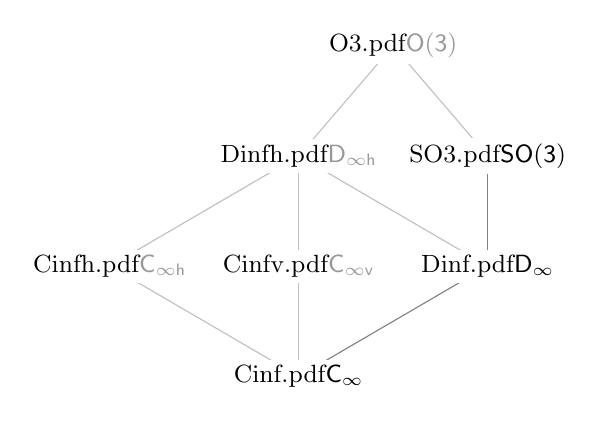
\begin{tikzpicture}[x=1cm, y=1cm, every node/.style={fill=white, font=\small, inner sep=2pt}]
\draw[black!25, line width=0.4pt] (0,0) -- (-2.4,1.4);
\draw[black!25, line width=0.4pt] (0,0) -- (0,1.4);
\draw[black!50, line width=0.4pt] (0,0) -- (2.4,1.4);
\draw[black!25, line width=0.4pt] (-2.4,1.4) -- (0,2.8);
\draw[black!25, line width=0.4pt] (0,1.4) -- (0,2.8);
\draw[black!25, line width=0.4pt] (2.4,1.4) -- (0,2.8);
\draw[black!50, line width=0.4pt] (2.4,1.4) -- (2.4,2.8);
\draw[black!25, line width=0.4pt] (0,2.8) -- (1.2,4.2);
\draw[black!25, line width=0.4pt] (2.4,2.8) -- (1.2,4.2);
\node at (0,0) {\href{Cinf.pdf}{\textcolor{black}{$\grp{C_{\infty}}$}}};
\node at (-2.4,1.4) {\href{Cinfh.pdf}{\textcolor{black!40}{$\grp{C_{\infty h}}$}}};
\node at (0,1.4) {\href{Cinfv.pdf}{\textcolor{black!40}{$\grp{C_{\infty v}}$}}};
\node at (2.4,1.4) {\href{Dinf.pdf}{\textcolor{black}{$\grp{D_{\infty}}$}}};
\node at (0,2.8) {\href{Dinfh.pdf}{\textcolor{black!40}{$\grp{D_{\infty h}}$}}};
\node at (2.4,2.8) {\href{SO3.pdf}{\textcolor{black}{$\grp{SO(3)}$}}};
\node at (1.2,4.2) {\href{O3.pdf}{\textcolor{black!40}{$\grp{O(3)}$}}};
\end{tikzpicture}\end{center}
\leavevmode\label{n:group.H}The table lists the closed subgroups $\grp{H}$ other than $\grp{SO(3)}$ up to conjugacy in $\grp{SO(3)}$, one in each row: the continuous subgroups, then the members of each family, then the exceptional groups. A row with $N$ in its symbol stands for every $N$ of its range, and its entries are functions of $N$. \label{n:head.subgroup}\label{n:head.order}\label{n:head.conjugates}\label{n:head.normal}A row gives $\grp{H}$ (subgrp), its order, the number of subgroups conjugate to $\grp{H}$ in $\grp{SO(3)}$ (conjugates) and whether $\grp{H}$ is normal. \label{n:group.normalizer}\label{n:group.centralizer}It also gives the normalizer $\grp{N}_{\hairsp \grp{SO(3)}}(\grp{H})$ and the centralizer $\grp{C}_{\hairsp \grp{SO(3)}}(\grp{H})$ in $\grp{SO(3)}$ (\texttt{normalizer}, \texttt{centralizer}). They are the normalizer and the centralizer in \href{O3.pdf}{$\grp{O(3)}$} intersected with $\grp{SO(3)}$. As $\elt{i}$ commutes with every element, every map of the record of $\grp{H}$ onto a subgroup given by a conjugation in \href{O3.pdf}{$\grp{O(3)}$} is also given by a conjugation in $\grp{SO(3)}$. Thus the restriction of $\irrJ{J}$ to $\grp{H}$ has one setting. A subgroup's other names in its \href{O3.pdf}{$\grp{O(3)}$}-conjugacy class follow $\samecls$ (\href{../../CONVENTIONS.pdf}{CONVENTIONS.pdf}, section \href{../../CONVENTIONS.pdf\#conv.2.1}{2.1}).
{\small\begin{longtable}{@{}lrrlll@{}}\toprule
subgrp & order & conjugates & normal & $\grp{N}_{\hairsp \grp{SO(3)}}(\grp{H})$ & $\grp{C}_{\hairsp \grp{SO(3)}}(\grp{H})$\\\midrule\endhead
\bottomrule\endfoot\endlastfoot
\href{Cinf.pdf}{$\grp{C_{\infty}}$} & $\infty$ & $\infty$ & no & \href{Dinf.pdf}{$\grp{D_{\infty}}$} & \href{Cinf.pdf}{$\grp{C_{\infty}}$}\\*
\href{Dinf.pdf}{$\grp{D_{\infty}}$} & $\infty$ & $\infty$ & no & \href{Dinf.pdf}{$\grp{D_{\infty}}$} & \href{C2.pdf}{$\grp{C_{2}}$}\\*
\grouprule{0pt}{\lightrulewidth}
\href{C1.pdf}{$\grp{C_{1}}$} & 1 & 1 & yes & \href{SO3.pdf}{$\grp{SO(3)}$} & \href{SO3.pdf}{$\grp{SO(3)}$}\\*
\href{C2.pdf}{$\grp{C_{2}}$} $\samecls$ \href{D1.pdf}{$\grp{D_{1}}$} & 2 & $\infty$ & no & \href{Dinf.pdf}{$\grp{D_{\infty}}$} & \href{Dinf.pdf}{$\grp{D_{\infty}}$}\\*
$\grp{C_{\mathnormal{N}}}$, $N \ge 3$ & $N$ & $\infty$ & no & \href{Dinf.pdf}{$\grp{D_{\infty}}$} & \href{Cinf.pdf}{$\grp{C_{\infty}}$}\\*
\grouprule{0pt}{\lightrulewidth}
\href{D2.pdf}{$\grp{D_{2}}$} & 4 & $\infty$ & no & \href{O.pdf}{$\grp{O}$} & \href{D2.pdf}{$\grp{D_{2}}$}\\*
$\grp{D_{\mathnormal{N}}}$, $N \ge 3$ & $2N$ & $\infty$ & no & $\grp{D_{2\mathnormal{N}}}$ & \href{C2.pdf}{$\grp{C_{2}}$}\\*
\grouprule{0pt}{\lightrulewidth}
\href{T.pdf}{$\grp{T}$} & 12 & $\infty$ & no & \href{O.pdf}{$\grp{O}$} & \href{C1.pdf}{$\grp{C_{1}}$}\\*
\href{O.pdf}{$\grp{O}$} & 24 & $\infty$ & no & \href{O.pdf}{$\grp{O}$} & \href{C1.pdf}{$\grp{C_{1}}$}\\*
\href{I.pdf}{$\grp{I}$} & 60 & $\infty$ & no & \href{I.pdf}{$\grp{I}$} & \href{C1.pdf}{$\grp{C_{1}}$}\\
\bottomrule\end{longtable}}
\needspace{103pt}
\section{Descent of symmetry}\label{s:subduction}
Conventions: \href{../../CONVENTIONS.pdf}{CONVENTIONS.pdf}, section \href{../../CONVENTIONS.pdf\#conv.16.1}{16.1}.
Below is the restriction of $\irrJ{J}$ to each closed subgroup $\grp{H}$ of $\grp{SO(3)}$ (section~\ref{s:subgroups}) for every $J$ (\texttt{subduction\symbol{95}rules}). \label{n:irrep.Gamma.subgroup}For an axial $\grp{H}$ it is the direct sum, over the kets $\jm{J}{m}$, of the terms of the first true case of its rule. For \href{Dinf.pdf}{$\grp{D_{\infty}}$} and $\grp{D_{\mathnormal{N}}}$, the sum runs over $\jm{J}{0}$ and the pairs $\jm{J}{\pm m}$, \mbox{$m > 0$}. \label{n:index.residue}\label{n:constant.root}In the rules, $q = m \bmod N$, and $\rootunity{N}^{q}$ is the character of $\jm{J}{m}$ on the rotation by $2\pi/N$ about $z$, where $\rootunity{N} = \expe^{2\pi\iunit/N}$. In the rules of a family, the terms and the irreps of the generating functions are irreps of the member of $\grp{C_{\mathnormal{N}}}$ or $\grp{D_{\mathnormal{N}}}$. They are labeled as in \href{../../CONVENTIONS.pdf}{CONVENTIONS.pdf}, section \href{../../CONVENTIONS.pdf\#conv.6.1}{6.1}, and for $N \le 2$ named as in \href{../../CONVENTIONS.pdf}{CONVENTIONS.pdf}, section \href{../../CONVENTIONS.pdf\#conv.6.3}{6.3}. \label{n:function.multiplicity}\label{n:irrep.Delta}\label{n:index.generating.variable}\label{n:function.generating}\label{n:function.generating.numerator}The multiplicity $b_\Lambda(J)$ of an irrep $\Lambda$ of $\grp{H}$ is the coefficient of $t^J$ in its generating function $H_\Lambda(t) = \sum_{J\ge0} b_\Lambda(J)\, t^J$. The generating functions are given for every $\grp{H}$, and without a rule for \href{T.pdf}{$\grp{T}$}, \href{O.pdf}{$\grp{O}$} and \href{I.pdf}{$\grp{I}$}. They use the same $q$, and $n$ is the index of a family of irreps of \href{Cinf.pdf}{$\grp{C_{\infty}}$} or \href{Dinf.pdf}{$\grp{D_{\infty}}$}. The document of each subgroup except the members with $N > 12$ lists the restrictions $J$ by $J$, in its section Subduction from \href{O3.pdf}{$\grp{O(3)}$}.
\needspace{95pt}
\paragraph{Continuous subgroups.}
{\small\renewcommand{\arraystretch}{1.6}\setlength{\fillwidth}{\textwidth}\addtolength{\fillwidth}{-2\tabcolsep}\setlength{\colwidth}{0pt}\cellmax{$H_\Lambda(t)$}\cellmax{$\irrJ{J}$}\addtolength{\fillwidth}{-\colwidth}\setlength{\colwidth}{0pt}\cellmax{$\bigoplus_{m=0}^{J}\Lambda_m$, $\Lambda_0$ on $\jm{J}{0}$ and $\Lambda_m$ on the pair $\jm{J}{\pm m}$ for \mbox{$m > 0$}: $\irr{a}_{1}$ if $m = 0$ and $J$ even, $\irr{a}_{2}$ if $m = 0$ and $J$ odd, $\irr{e}_{m}$ otherwise}\cellmax{$\bigoplus_{m=-J}^{J}\Lambda_m$, $\Lambda_m$ on $\jm{J}{m}$: $\irr{a}$ if $m = 0$, $\conjpair{1}\irr{e}_{m}$ if $m > 0$, $\conjpair{2}\irr{e}_{-m}$ if $m < 0$}\cellmax{$1/(1-t^{2})$ for $\irr{a}_{1}$, $t/(1-t^{2})$ for $\irr{a}_{2}$, $t^{n}/(1-t)$ for $\irr{e}_{n}$}\cellmax{$1/(1-t)$ for $\irr{a}$, $t^{n}/(1-t)$ for $\conjpair{1}\irr{e}_{n}$ and $\conjpair{2}\irr{e}_{n}$}\fillcap\begin{longtable}{@{}l>{\raggedright\arraybackslash}p{\fillwidth}@{}}\toprule
\multicolumn{2}{@{}c@{}}{\href{Cinf.pdf}{$\grp{C_{\infty}}$}}\\*
$\irrJ{J}$ & $\bigoplus_{m=-J}^{J}\Lambda_m$, $\Lambda_m$ on $\jm{J}{m}$: $\irr{a}$ if $m = 0$, $\conjpair{1}\irr{e}_{m}$ if $m > 0$, $\conjpair{2}\irr{e}_{-m}$ if $m < 0$\\*
$H_\Lambda(t)$ & $1/(1-t)$ for $\irr{a}$, $t^{n}/(1-t)$ for $\conjpair{1}\irr{e}_{n}$ and $\conjpair{2}\irr{e}_{n}$\\
\grouprule{0pt}{\lightrulewidth}
\multicolumn{2}{@{}c@{}}{\href{Dinf.pdf}{$\grp{D_{\infty}}$}}\\*
$\irrJ{J}$ & $\bigoplus_{m=0}^{J}\Lambda_m$, $\Lambda_0$ on $\jm{J}{0}$ and $\Lambda_m$ on the pair $\jm{J}{\pm m}$ for \mbox{$m > 0$}: $\irr{a}_{1}$ if $m = 0$ and $J$ even, $\irr{a}_{2}$ if $m = 0$ and $J$ odd, $\irr{e}_{m}$ otherwise\\*
$H_\Lambda(t)$ & $1/(1-t^{2})$ for $\irr{a}_{1}$, $t/(1-t^{2})$ for $\irr{a}_{2}$, $t^{n}/(1-t)$ for $\irr{e}_{n}$\\
\bottomrule\end{longtable}}
\needspace{95pt}
\paragraph{Subduction to the $\grp{C_{\mathnormal{N}}}$ family.}
{\small\renewcommand{\arraystretch}{1.6}\setlength{\fillwidth}{\textwidth}\addtolength{\fillwidth}{-2\tabcolsep}\setlength{\colwidth}{0pt}\cellmax{$H_\Lambda(t)$}\cellmax{$\irrJ{J}$}\addtolength{\fillwidth}{-\colwidth}\setlength{\colwidth}{0pt}\cellmax{$P_\Lambda(t)/((1-t)(1-t^{N}))$, $P_\Lambda(t)$: $1 + t^{N}$ for $\irr{a}$, $2t^{N/2}$ for $\irr{b}$ ($N$ even), $t^{q} + t^{N-q}$ for $\conjpair{1}\irr{e}_{q}$ ($0 < q < N/2$) and $\conjpair{2}\irr{e}_{N-q}$ ($N/2 < q < N$)}\cellmax{$\bigoplus_{m=-J}^{J}\Lambda_m$, $\Lambda_m$ on $\jm{J}{m}$: $\irr{a}$ if $q = 0$, $\irr{b}$ if $q = N/2$, $\conjpair{1}\irr{e}_{q}$ if $0 < q < N/2$, $\conjpair{2}\irr{e}_{N-q}$ if $N/2 < q < N$; $q = m \bmod N$}\fillcap\begin{longtable}{@{}l>{\raggedright\arraybackslash}p{\fillwidth}@{}}\toprule
\multicolumn{2}{@{}c@{}}{every $N$}\\*
$\irrJ{J}$ & $\bigoplus_{m=-J}^{J}\Lambda_m$, $\Lambda_m$ on $\jm{J}{m}$: $\irr{a}$ if $q = 0$, $\irr{b}$ if $q = N/2$, $\conjpair{1}\irr{e}_{q}$ if $0 < q < N/2$, $\conjpair{2}\irr{e}_{N-q}$ if $N/2 < q < N$; $q = m \bmod N$\\*
$H_\Lambda(t)$ & $P_\Lambda(t)/((1-t)(1-t^{N}))$, $P_\Lambda(t)$: $1 + t^{N}$ for $\irr{a}$, $2t^{N/2}$ for $\irr{b}$ ($N$ even), $t^{q} + t^{N-q}$ for $\conjpair{1}\irr{e}_{q}$ ($0 < q < N/2$) and $\conjpair{2}\irr{e}_{N-q}$ ($N/2 < q < N$)\\
\bottomrule\end{longtable}}
\needspace{95pt}
\paragraph{Subduction to the $\grp{D_{\mathnormal{N}}}$ family.}
{\small\renewcommand{\arraystretch}{1.6}\setlength{\fillwidth}{\textwidth}\addtolength{\fillwidth}{-2\tabcolsep}\setlength{\colwidth}{0pt}\cellmax{$H_\Lambda(t)$}\cellmax{$\irrJ{J}$}\addtolength{\fillwidth}{-\colwidth}\setlength{\colwidth}{0pt}\cellmax{$\bigoplus_{m=0}^{J}\Lambda_m$, $\Lambda_0$ on $\jm{J}{0}$ and $\Lambda_m$ on the pair $\jm{J}{\pm m}$ for \mbox{$m > 0$}: $\irr{a}_{1}$ if $m = 0$ and $J$ even, $\irr{a}_{2}$ if $m = 0$ and $J$ odd, $\irr{a}_{1}\oplus \irr{a}_{2}$ if $q = 0$, $\irr{b}_{1}\oplus \irr{b}_{2}$ if $q = N/2$, $\irr{e}_{\min(q, N-q)}$ otherwise; $q = m \bmod N$}\cellmax{$P_\Lambda(t)/((1-t^{2})(1-t^{N}))$, $P_\Lambda(t)$: $1 + t^{N+1}$ for $\irr{a}_{1}$, $t + t^{N}$ for $\irr{a}_{2}$, $t^{N/2} + t^{N/2+1}$ for $\irr{b}_{1}$ and $\irr{b}_{2}$ ($N$ even), $t^{q} + t^{q+1} + t^{N-q} + t^{N-q+1}$ for $\irr{e}_{q}$ ($0 < q < N/2$)}\fillcap\begin{longtable}{@{}l>{\raggedright\arraybackslash}p{\fillwidth}@{}}\toprule
\multicolumn{2}{@{}c@{}}{every $N \ge 2$}\\*
$\irrJ{J}$ & $\bigoplus_{m=0}^{J}\Lambda_m$, $\Lambda_0$ on $\jm{J}{0}$ and $\Lambda_m$ on the pair $\jm{J}{\pm m}$ for \mbox{$m > 0$}: $\irr{a}_{1}$ if $m = 0$ and $J$ even, $\irr{a}_{2}$ if $m = 0$ and $J$ odd, $\irr{a}_{1}\oplus \irr{a}_{2}$ if $q = 0$, $\irr{b}_{1}\oplus \irr{b}_{2}$ if $q = N/2$, $\irr{e}_{\min(q, N-q)}$ otherwise; $q = m \bmod N$\\*
$H_\Lambda(t)$ & $P_\Lambda(t)/((1-t^{2})(1-t^{N}))$, $P_\Lambda(t)$: $1 + t^{N+1}$ for $\irr{a}_{1}$, $t + t^{N}$ for $\irr{a}_{2}$, $t^{N/2} + t^{N/2+1}$ for $\irr{b}_{1}$ and $\irr{b}_{2}$ ($N$ even), $t^{q} + t^{q+1} + t^{N-q} + t^{N-q+1}$ for $\irr{e}_{q}$ ($0 < q < N/2$)\\
\bottomrule\end{longtable}}
\needspace{249pt}
\paragraph{Subduction to $\grp{T}$, $\grp{O}$ and $\grp{I}$.} The generating functions are
\begin{equation}\label{e:gftoi}H_\Lambda(t) = P_\Lambda(t)/((1-t^{3})(1-t^{4}))\ \text{for } \grp{T},\quad P_\Lambda(t)/((1-t^{4})(1-t^{6}))\ \text{for } \grp{O},\quad P_\Lambda(t)/((1-t^{6})(1-t^{10}))\ \text{for } \grp{I}.\end{equation}
{\small\begin{longtable}{@{}ll@{\hspace{18pt}}ll@{}}\toprule
$\Lambda$ & $P_\Lambda(t)$ & $\Lambda$ & $P_\Lambda(t)$\\\midrule\endhead
\bottomrule\endfoot\endlastfoot
\multicolumn{2}{@{}c@{\hspace{18pt}}}{\href{T.pdf}{$\grp{T}$}} & \multicolumn{2}{@{}c@{}}{\href{I.pdf}{$\grp{I}$}}\\*
$\irr{a}$ & $1 + t^{6}$ & $\irr{a}$ & $1 + t^{15}$\\*
$\conjpair{1}\irr{e}$ & $t^{2} + t^{4}$ & $\irr{t}_{1}$ & $t + t^{5} + t^{6} + t^{9} + t^{10} + t^{14}$\\*
$\conjpair{2}\irr{e}$ & $t^{2} + t^{4}$ & $\irr{t}_{2}$ & $t^{3} + t^{5} + t^{7} + t^{8} + t^{10} + t^{12}$\\*
$\irr{t}$ & $t + t^{2} + 2t^{3} + t^{4} + t^{5}$ & $\irr{g}$ & $t^{3} + t^{4} + t^{6} + t^{7} + t^{8} + t^{9} + t^{11} + t^{12}$\\*\noalign{\vskip 1.5pt}\multispan{2}\leaders\hrule height\cmidrulewidth\hfill\kern0pt\hskip18pt & \multispan{2}\\*\noalign{\vskip 1.5pt}
\multicolumn{2}{@{}c@{\hspace{18pt}}}{\href{O.pdf}{$\grp{O}$}} & $\irr{h}$ & $t^{2} + t^{4} + t^{5} + t^{6} + t^{7} + t^{8} + t^{9} + t^{10} + t^{11} + t^{13}$\\*
$\irr{a}_{1}$ & $1 + t^{9}$ &  & \\*
$\irr{a}_{2}$ & $t^{3} + t^{6}$ &  & \\*
$\irr{e}$ & $t^{2} + t^{4} + t^{5} + t^{7}$ &  & \\*
$\irr{t}_{1}$ & $t + t^{3} + t^{4} + t^{5} + t^{6} + t^{8}$ &  & \\*
$\irr{t}_{2}$ & $t^{2} + t^{3} + t^{4} + t^{5} + t^{6} + t^{7}$ &  & \\
\bottomrule\end{longtable}}
\needspace{177pt}
\partbox{Angular momentum}
\section{Subduction from \texorpdfstring{$\grp{O(3)}$}{O(3)}}\label{s:subduction_o3}
Conventions: \href{../../CONVENTIONS.pdf}{CONVENTIONS.pdf}, section \href{../../CONVENTIONS.pdf\#conv.11}{11}.
\leavevmode\label{n:index.parity}The irrep $\irrJp{J}{p}$ of \href{O3.pdf}{$\grp{O(3)}$} has angular momentum $J$ and parity $p$ ($\ptag{g}$ for $p = +1$, $\ptag{u}$ for $p = -1$). For every $J$,
\begin{equation}\label{e:o3rule}\restr{\irrJp{J}{p}}{\grp{SO(3)}} = \irrJ{J}\quad\text{for both } p.\end{equation}
The record also holds the restrictions for $J \le 12$ (\texttt{subduction\symbol{95}o3.instances}).
\needspace{110pt}
\section{Multiplicities and allowed \texorpdfstring{$m$}{m}}\label{s:multiplicities}
Conventions: \href{../../CONVENTIONS.pdf}{CONVENTIONS.pdf}, section \href{../../CONVENTIONS.pdf\#conv.14}{14}.
The multiplicity $b_\Gamma(J)$ is the number of blocks of $\Gamma$ at $J$, with the generating function
\begin{equation}\label{e:gf}H_\Gamma(t) = \sum_{J\ge0} b_\Gamma(J)\,t^J,\end{equation}
\leavevmode\label{n:head.parity}for each family's instance of index $J$. This instance can only have a block at the angular momentum $J$. The column $m$ gives the $m$ of the kets of $\Gamma$.
\begin{center}\small\begin{tabular}{@{}lllll@{}}\toprule
family & $H_\Gamma(t)$ & $b_\Gamma(J)$, $J$ even & $J$ odd & $m$\\\midrule
$\irrJ{J}$ & $t^{J}$ & $1$ & $1$ & $J, J-1, \dots, -J$\\
\bottomrule\end{tabular}\end{center}
\needspace{110pt}
\section{Symmetry-adapted bases}\label{s:bases}
Conventions: \href{../../CONVENTIONS.pdf}{CONVENTIONS.pdf}, section \href{../../CONVENTIONS.pdf\#conv.14.1}{14.1}.
\leavevmode\label{n:index.m}\label{n:vector.ket}The kets $\jm{J}{m}$ are the spherical harmonics (the inversion acts as $(-1)^J$). \label{n:index.ketcoefficient}\label{n:vector.basis.symmetry}\label{n:index.ketweight}\label{n:index.total}A vector is listed by its coefficients $e_m$:
\begin{equation}\label{e:ket}v = \frac{1}{\sqrt{\mathrm{tot}}}\sum_m e_m\sqrt{F_m}\;\jm{J}{m},\qquad F_m = (J+m)!\,(J-m)!,\qquad \mathrm{tot} = \sum_m |e_m|^2F_m,\end{equation}
so a vector here is a single ket, $e_m = 1$, of amplitude 1.
The restriction $\restr{\irrJp{J}{p}}{\grp{SO(3)}}$ is irreducible for every $J$ and $p$, so the block of $J$ contains all the $2J+1$ kets $\jm{J}{m}$. The ket $\jm{J}{m}$ is the partner $\intx = J - m + 1$, $m = J, J-1, \dots, -J$, and the block's irrep is $\irrJ{J}$. Blocks are ordered by $J$. \label{n:head.case}\label{n:head.partners}The table lists every case of block, its dimension $d$ and its partners in order.
\begin{center}\begin{tabular}{@{}lrl@{}}\toprule
case & $d$ & partners\\\midrule
every $J$ & $2J+1$ & $\jm{J}{J}, \jm{J}{J-1}, \dots, \jm{J}{-J}$\\
\bottomrule\end{tabular}\end{center}
The bases have 11 blocks and 121 vectors at $J = 0, 1, \dots, 10$. \label{n:index.copy}\label{n:head.irrep}A row gives a block at $J$: its irrep, its copy index $\mult$, its dimension $d$ and its partners.
{\small\setlength{\tabcolsep}{3pt}\setlength{\fillwidth}{\textwidth}\addtolength{\fillwidth}{-\dimexpr 6\tabcolsep+6pt\relax}\setlength{\colwidth}{0pt}\cellmax{10}\cellmax{$J$}\cellmax{0}\cellmax{1}\cellmax{2}\cellmax{3}\cellmax{4}\cellmax{5}\cellmax{6}\cellmax{7}\cellmax{8}\cellmax{9}\addtolength{\fillwidth}{-\colwidth}\setlength{\colwidth}{0pt}\cellmax{$\irrJ{10}$}\cellmax{irrep}\cellmax{$\irrJ{0}$}\cellmax{$\irrJ{1}$}\cellmax{$\irrJ{2}$}\cellmax{$\irrJ{3}$}\cellmax{$\irrJ{4}$}\cellmax{$\irrJ{5}$}\cellmax{$\irrJ{6}$}\cellmax{$\irrJ{7}$}\cellmax{$\irrJ{8}$}\cellmax{$\irrJ{9}$}\addtolength{\fillwidth}{-\colwidth}\setlength{\colwidth}{0pt}\cellmax{$\mult$}\cellmax{1}\addtolength{\fillwidth}{-\colwidth}\setlength{\colwidth}{0pt}\cellmax{11}\cellmax{13}\cellmax{15}\cellmax{17}\cellmax{19}\cellmax{21}\cellmax{$d$}\cellmax{1}\cellmax{3}\cellmax{5}\cellmax{7}\cellmax{9}\addtolength{\fillwidth}{-\colwidth}\setlength{\colwidth}{0pt}\cellmax{$\jm{10}{10}$, $\jm{10}{9}$, $\jm{10}{8}$, $\jm{10}{7}$, $\jm{10}{6}$, $\jm{10}{5}$, $\jm{10}{4}$, $\jm{10}{3}$, $\jm{10}{2}$, $\jm{10}{1}$, $\jm{10}{0}$, $\jm{10}{-1}$, $\jm{10}{-2}$, $\jm{10}{-3}$, $\jm{10}{-4}$, $\jm{10}{-5}$, $\jm{10}{-6}$, $\jm{10}{-7}$, $\jm{10}{-8}$, $\jm{10}{-9}$, $\jm{10}{-10}$}\cellmax{$\jm{9}{9}$, $\jm{9}{8}$, $\jm{9}{7}$, $\jm{9}{6}$, $\jm{9}{5}$, $\jm{9}{4}$, $\jm{9}{3}$, $\jm{9}{2}$, $\jm{9}{1}$, $\jm{9}{0}$, $\jm{9}{-1}$, $\jm{9}{-2}$, $\jm{9}{-3}$, $\jm{9}{-4}$, $\jm{9}{-5}$, $\jm{9}{-6}$, $\jm{9}{-7}$, $\jm{9}{-8}$, $\jm{9}{-9}$}\cellmax{$\jm{8}{8}$, $\jm{8}{7}$, $\jm{8}{6}$, $\jm{8}{5}$, $\jm{8}{4}$, $\jm{8}{3}$, $\jm{8}{2}$, $\jm{8}{1}$, $\jm{8}{0}$, $\jm{8}{-1}$, $\jm{8}{-2}$, $\jm{8}{-3}$, $\jm{8}{-4}$, $\jm{8}{-5}$, $\jm{8}{-6}$, $\jm{8}{-7}$, $\jm{8}{-8}$}\cellmax{$\jm{7}{7}$, $\jm{7}{6}$, $\jm{7}{5}$, $\jm{7}{4}$, $\jm{7}{3}$, $\jm{7}{2}$, $\jm{7}{1}$, $\jm{7}{0}$, $\jm{7}{-1}$, $\jm{7}{-2}$, $\jm{7}{-3}$, $\jm{7}{-4}$, $\jm{7}{-5}$, $\jm{7}{-6}$, $\jm{7}{-7}$}\cellmax{$\jm{6}{6}$, $\jm{6}{5}$, $\jm{6}{4}$, $\jm{6}{3}$, $\jm{6}{2}$, $\jm{6}{1}$, $\jm{6}{0}$, $\jm{6}{-1}$, $\jm{6}{-2}$, $\jm{6}{-3}$, $\jm{6}{-4}$, $\jm{6}{-5}$, $\jm{6}{-6}$}\cellmax{$\jm{5}{5}$, $\jm{5}{4}$, $\jm{5}{3}$, $\jm{5}{2}$, $\jm{5}{1}$, $\jm{5}{0}$, $\jm{5}{-1}$, $\jm{5}{-2}$, $\jm{5}{-3}$, $\jm{5}{-4}$, $\jm{5}{-5}$}\cellmax{$\jm{4}{4}$, $\jm{4}{3}$, $\jm{4}{2}$, $\jm{4}{1}$, $\jm{4}{0}$, $\jm{4}{-1}$, $\jm{4}{-2}$, $\jm{4}{-3}$, $\jm{4}{-4}$}\cellmax{$\jm{3}{3}$, $\jm{3}{2}$, $\jm{3}{1}$, $\jm{3}{0}$, $\jm{3}{-1}$, $\jm{3}{-2}$, $\jm{3}{-3}$}\cellmax{$\jm{2}{2}$, $\jm{2}{1}$, $\jm{2}{0}$, $\jm{2}{-1}$, $\jm{2}{-2}$}\cellmax{partners $\intx = 1, 2, \dots, d$}\cellmax{$\jm{1}{1}$, $\jm{1}{0}$, $\jm{1}{-1}$}\cellmax{$\jm{0}{0}$}\fillcap\begin{longtable}{@{}rlrr@{\hspace{6pt}}p{\fillwidth}@{}}\toprule
$J$ & irrep & $\mult$ & $d$ & partners $\intx = 1, 2, \dots, d$\\\midrule\endhead
\bottomrule\endfoot\endlastfoot
0 & $\irrJ{0}$ & 1 & 1 & $\jm{0}{0}$\\*
1 & $\irrJ{1}$ & 1 & 3 & $\jm{1}{1}$, $\jm{1}{0}$, $\jm{1}{-1}$\\
2 & $\irrJ{2}$ & 1 & 5 & $\jm{2}{2}$, $\jm{2}{1}$, $\jm{2}{0}$, $\jm{2}{-1}$, $\jm{2}{-2}$\\
3 & $\irrJ{3}$ & 1 & 7 & $\jm{3}{3}$, $\jm{3}{2}$, $\jm{3}{1}$, $\jm{3}{0}$, $\jm{3}{-1}$, $\jm{3}{-2}$, $\jm{3}{-3}$\\
4 & $\irrJ{4}$ & 1 & 9 & $\jm{4}{4}$, $\jm{4}{3}$, $\jm{4}{2}$, $\jm{4}{1}$, $\jm{4}{0}$, $\jm{4}{-1}$, $\jm{4}{-2}$, $\jm{4}{-3}$, $\jm{4}{-4}$\\
5 & $\irrJ{5}$ & 1 & 11 & $\jm{5}{5}$, $\jm{5}{4}$, $\jm{5}{3}$, $\jm{5}{2}$, $\jm{5}{1}$, $\jm{5}{0}$, $\jm{5}{-1}$, $\jm{5}{-2}$, $\jm{5}{-3}$, $\jm{5}{-4}$, $\jm{5}{-5}$\\
6 & $\irrJ{6}$ & 1 & 13 & $\jm{6}{6}$, $\jm{6}{5}$, $\jm{6}{4}$, $\jm{6}{3}$, $\jm{6}{2}$, $\jm{6}{1}$, $\jm{6}{0}$, $\jm{6}{-1}$, $\jm{6}{-2}$, $\jm{6}{-3}$, $\jm{6}{-4}$, $\jm{6}{-5}$, $\jm{6}{-6}$\\
7 & $\irrJ{7}$ & 1 & 15 & $\jm{7}{7}$, $\jm{7}{6}$, $\jm{7}{5}$, $\jm{7}{4}$, $\jm{7}{3}$, $\jm{7}{2}$, $\jm{7}{1}$, $\jm{7}{0}$, $\jm{7}{-1}$, $\jm{7}{-2}$, $\jm{7}{-3}$, $\jm{7}{-4}$, $\jm{7}{-5}$, $\jm{7}{-6}$, $\jm{7}{-7}$\\
8 & $\irrJ{8}$ & 1 & 17 & $\jm{8}{8}$, $\jm{8}{7}$, $\jm{8}{6}$, $\jm{8}{5}$, $\jm{8}{4}$, $\jm{8}{3}$, $\jm{8}{2}$, $\jm{8}{1}$, $\jm{8}{0}$, $\jm{8}{-1}$, $\jm{8}{-2}$, $\jm{8}{-3}$, $\jm{8}{-4}$, $\jm{8}{-5}$, $\jm{8}{-6}$, $\jm{8}{-7}$, $\jm{8}{-8}$\\
9 & $\irrJ{9}$ & 1 & 19 & $\jm{9}{9}$, $\jm{9}{8}$, $\jm{9}{7}$, $\jm{9}{6}$, $\jm{9}{5}$, $\jm{9}{4}$, $\jm{9}{3}$, $\jm{9}{2}$, $\jm{9}{1}$, $\jm{9}{0}$, $\jm{9}{-1}$, $\jm{9}{-2}$, $\jm{9}{-3}$, $\jm{9}{-4}$, $\jm{9}{-5}$, $\jm{9}{-6}$, $\jm{9}{-7}$, $\jm{9}{-8}$, $\jm{9}{-9}$\\*
10 & $\irrJ{10}$ & 1 & 21 & $\jm{10}{10}$, $\jm{10}{9}$, $\jm{10}{8}$, $\jm{10}{7}$, $\jm{10}{6}$, $\jm{10}{5}$, $\jm{10}{4}$, $\jm{10}{3}$, $\jm{10}{2}$, $\jm{10}{1}$, $\jm{10}{0}$, $\jm{10}{-1}$, $\jm{10}{-2}$, $\jm{10}{-3}$, $\jm{10}{-4}$, $\jm{10}{-5}$, $\jm{10}{-6}$, $\jm{10}{-7}$, $\jm{10}{-8}$, $\jm{10}{-9}$, $\jm{10}{-10}$\\
\bottomrule\end{longtable}}
\needspace{323pt}
\partbox{Tensors}
\section{\texorpdfstring{$\orbital{s}$, $\orbital{p}$, $\orbital{d}$, $\orbital{f}$}{s, p, d, f} functions}\label{s:orbitals}
Conventions: \href{../../CONVENTIONS.pdf}{CONVENTIONS.pdf}, section \href{../../CONVENTIONS.pdf\#conv.13}{13}.
\leavevmode\label{n:head.function}A function is a real solid harmonic $\orbital{s}$, $\orbital{p}$, $\orbital{d}$ or $\orbital{f}$, of degree 0 to 3 with coprime integer coefficients, or a component $\orbital{R}_{x}$, $\orbital{R}_{y}$, $\orbital{R}_{z}$ of an axial vector. \label{n:head.polynomial}\label{n:head.irreps}A row gives the function, its polynomial in $x$, $y$ and $z$, and the irreps of its nonzero isotypic components.
{\small\begin{longtable}{@{}lll@{\hspace{18pt}}lll@{}}\toprule
function & polynomial & irreps & function & polynomial & irreps\\\midrule\endhead
\bottomrule\endfoot\endlastfoot
$\orbital{s}$ & $1$ & $\irrJ{0}$ & $\orbital{f}_{xz^2}$ & $-x^{3} - xy^{2} + 4xz^{2}$ & $\irrJ{3}$\\*
$\orbital{p}_{x}$ & $x$ & $\irrJ{1}$ & $\orbital{f}_{yz^2}$ & $-x^{2}y - y^{3} + 4yz^{2}$ & $\irrJ{3}$\\*
$\orbital{p}_{y}$ & $y$ & $\irrJ{1}$ & $\orbital{f}_{z(x^2-y^2)}$ & $x^{2}z - y^{2}z$ & $\irrJ{3}$\\*
$\orbital{p}_{z}$ & $z$ & $\irrJ{1}$ & $\orbital{f}_{xyz}$ & $xyz$ & $\irrJ{3}$\\*
$\orbital{d}_{z^2}$ & $-x^{2} - y^{2} + 2z^{2}$ & $\irrJ{2}$ & $\orbital{f}_{x(x^2-3y^2)}$ & $x^{3} - 3xy^{2}$ & $\irrJ{3}$\\*
$\orbital{d}_{x^2-y^2}$ & $x^{2} - y^{2}$ & $\irrJ{2}$ & $\orbital{f}_{y(3x^2-y^2)}$ & $3x^{2}y - y^{3}$ & $\irrJ{3}$\\*
$\orbital{d}_{xy}$ & $xy$ & $\irrJ{2}$ & $\orbital{R}_{x}$ & $x$ & $\irrJ{1}$\\*
$\orbital{d}_{yz}$ & $yz$ & $\irrJ{2}$ & $\orbital{R}_{y}$ & $y$ & $\irrJ{1}$\\*
$\orbital{d}_{zx}$ & $xz$ & $\irrJ{2}$ & $\orbital{R}_{z}$ & $z$ & $\irrJ{1}$\\*
$\orbital{f}_{z^3}$ & $-3x^{2}z - 3y^{2}z + 2z^{3}$ & $\irrJ{3}$ &  &  & \\
\bottomrule\end{longtable}}
\needspace{247pt}
\needspace{103pt}
\section{Tensor spaces}\label{s:tensor_spaces}
Conventions: \href{../../CONVENTIONS.pdf}{CONVENTIONS.pdf}, section \href{../../CONVENTIONS.pdf\#conv.13}{13}.
\leavevmode\label{n:head.name}\label{n:head.description}\label{n:head.dim}\label{n:head.decomposition}A row is a space of Cartesian tensors, with its Jahn symbol (name), its description in words, its dimension (dim) and the irreps of $\grp{SO(3)}$ that it carries, with their multiplicities (decomposition). \label{n:label.jahn}The same symbol names the space in the isotypic components (V a polar vector, e an axial factor, a power the number of factors, brackets their symmetrized product). The descriptions name the symmetric polar tensors of a rank (the homogeneous polynomials of that degree), the axial vectors and the symmetric axial tensors of ranks 2 (optical activity) and 3. The elastic stiffness tensors are symmetric in their first two indices, in their last two and under the exchange of the two pairs. The photoelastic tensors are symmetric in their first two and in their last two indices, as are the electrostriction and the quadratic electro-optic tensors. The piezoelectric tensors are symmetric in their last two indices, the third-harmonic susceptibilities in their last three and the electrogyration tensors, which are axial, in their first two. The general polar tensors of rank 4 have no symmetry.
{\small\setlength{\fillwidth}{\textwidth}\addtolength{\fillwidth}{-6\tabcolsep}\setlength{\colwidth}{0pt}\cellmax{$\jahn{[[V^{2}]^{2}]}$}\cellmax{$\jahn{e[V^{2}]V}$}\cellmax{$\jahn{V[V^{2}]}$}\cellmax{$\jahn{V[V^{3}]}$}\cellmax{$\jahn{[V^{2}]^{2}}$}\cellmax{$\jahn{e[V^{2}]}$}\cellmax{$\jahn{e[V^{3}]}$}\cellmax{$\jahn{[V^{2}]}$}\cellmax{$\jahn{[V^{3}]}$}\cellmax{$\jahn{[V^{4}]}$}\cellmax{name}\cellmax{$\jahn{V^{0}}$}\cellmax{$\jahn{V^{4}}$}\cellmax{$\jahn{eV}$}\cellmax{$\jahn{V}$}\addtolength{\fillwidth}{-\colwidth}\setlength{\colwidth}{0pt}\cellmax{third-harmonic susceptibilities}\cellmax{symmetric axial tensors, rank 2}\cellmax{symmetric axial tensors, rank 3}\cellmax{symmetric polar tensors, rank 2}\cellmax{symmetric polar tensors, rank 3}\cellmax{symmetric polar tensors, rank 4}\cellmax{general polar tensors, rank 4}\cellmax{elastic stiffness tensors}\cellmax{electrogyration tensors}\cellmax{piezoelectric tensors}\cellmax{photoelastic tensors}\cellmax{axial vectors}\cellmax{polar vectors}\cellmax{description}\cellmax{scalars}\addtolength{\fillwidth}{-\colwidth}\setlength{\colwidth}{0pt}\cellmax{dim}\cellmax{10}\cellmax{15}\cellmax{18}\cellmax{21}\cellmax{30}\cellmax{36}\cellmax{81}\cellmax{1}\cellmax{3}\cellmax{6}\addtolength{\fillwidth}{-\colwidth}\setlength{\colwidth}{0pt}\cellmax{$3\,\irrJ{0} \oplus\allowbreak 6\,\irrJ{1} \oplus\allowbreak 6\,\irrJ{2} \oplus\allowbreak 3\,\irrJ{3} \oplus\allowbreak \irrJ{4}$}\cellmax{$2\,\irrJ{0} \oplus\allowbreak \irrJ{1} \oplus\allowbreak 3\,\irrJ{2} \oplus\allowbreak \irrJ{3} \oplus\allowbreak \irrJ{4}$}\cellmax{$\irrJ{0} \oplus\allowbreak \irrJ{1} \oplus\allowbreak 2\,\irrJ{2} \oplus\allowbreak \irrJ{3} \oplus\allowbreak \irrJ{4}$}\cellmax{$2\,\irrJ{0} \oplus\allowbreak 2\,\irrJ{2} \oplus\allowbreak \irrJ{4}$}\cellmax{$2\,\irrJ{1} \oplus\allowbreak \irrJ{2} \oplus\allowbreak \irrJ{3}$}\cellmax{$\irrJ{0} \oplus\allowbreak \irrJ{2} \oplus\allowbreak \irrJ{4}$}\cellmax{decomposition}\cellmax{$\irrJ{0} \oplus\allowbreak \irrJ{2}$}\cellmax{$\irrJ{1} \oplus\allowbreak \irrJ{3}$}\cellmax{$\irrJ{0}$}\cellmax{$\irrJ{1}$}\fillcap\begin{longtable}{@{}llr>{\RaggedRight\arraybackslash}p{\fillwidth}@{}}\toprule
name & description & dim & decomposition\\\midrule\endhead
\bottomrule\endfoot\endlastfoot
$\jahn{V^{0}}$ & scalars & 1 & $\irrJ{0}$\\*
$\jahn{V}$ & polar vectors & 3 & $\irrJ{1}$\\
$\jahn{[V^{2}]}$ & symmetric polar tensors, rank 2 & 6 & $\irrJ{0} \oplus\allowbreak \irrJ{2}$\\
$\jahn{[V^{3}]}$ & symmetric polar tensors, rank 3 & 10 & $\irrJ{1} \oplus\allowbreak \irrJ{3}$\\
$\jahn{[V^{4}]}$ & symmetric polar tensors, rank 4 & 15 & $\irrJ{0} \oplus\allowbreak \irrJ{2} \oplus\allowbreak \irrJ{4}$\\
$\jahn{eV}$ & axial vectors & 3 & $\irrJ{1}$\\
$\jahn{e[V^{2}]}$ & symmetric axial tensors, rank 2 & 6 & $\irrJ{0} \oplus\allowbreak \irrJ{2}$\\
$\jahn{e[V^{3}]}$ & symmetric axial tensors, rank 3 & 10 & $\irrJ{1} \oplus\allowbreak \irrJ{3}$\\
$\jahn{[[V^{2}]^{2}]}$ & elastic stiffness tensors & 21 & $2\,\irrJ{0} \oplus\allowbreak 2\,\irrJ{2} \oplus\allowbreak \irrJ{4}$\\
$\jahn{V[V^{2}]}$ & piezoelectric tensors & 18 & $2\,\irrJ{1} \oplus\allowbreak \irrJ{2} \oplus\allowbreak \irrJ{3}$\\
$\jahn{e[V^{2}]V}$ & electrogyration tensors & 18 & $2\,\irrJ{1} \oplus\allowbreak \irrJ{2} \oplus\allowbreak \irrJ{3}$\\
$\jahn{[V^{2}]^{2}}$ & photoelastic tensors & 36 & $2\,\irrJ{0} \oplus\allowbreak \irrJ{1} \oplus\allowbreak 3\,\irrJ{2} \oplus\allowbreak \irrJ{3} \oplus\allowbreak \irrJ{4}$\\
$\jahn{V[V^{3}]}$ & third-harmonic susceptibilities & 30 & $\irrJ{0} \oplus\allowbreak \irrJ{1} \oplus\allowbreak 2\,\irrJ{2} \oplus\allowbreak \irrJ{3} \oplus\allowbreak \irrJ{4}$\\*
$\jahn{V^{4}}$ & general polar tensors, rank 4 & 81 & $3\,\irrJ{0} \oplus\allowbreak 6\,\irrJ{1} \oplus\allowbreak 6\,\irrJ{2} \oplus\allowbreak 3\,\irrJ{3} \oplus\allowbreak \irrJ{4}$\\
\bottomrule\end{longtable}}
\needspace{235pt}
\needspace{103pt}
\section{Isotypic components}\label{s:isotypic}
Conventions: \href{../../CONVENTIONS.pdf}{CONVENTIONS.pdf}, section \href{../../CONVENTIONS.pdf\#conv.13}{13}.
\leavevmode\label{n:head.multiplicity}A row is an isotypic component, with the Jahn symbol of its space (name, as in the tensor spaces), its irrep, the multiplicity of the irrep in the space (mult.) and the component's dimension (dim). \label{n:head.coefficients}\label{n:head.basis}It also gives the field of the coefficients of its basis, rational or cyclotomic, and its reduced row echelon basis. \label{n:matrix.elastic}\label{n:matrix.piezoelectric}\label{n:matrix.electrogyration}\label{n:matrix.photoelastic}\label{n:matrix.susceptibility}A basis tensor of the elastic, piezoelectric, electrogyration or photoelastic tensors or of the third-harmonic susceptibilities is a combination of their coordinates, in this order, $c_{11}, \dots, c_{66}$, $d_{11}, \dots, d_{36}$, $\mathnormal{g}_{11}, \dots, \mathnormal{g}_{63}$, $p_{11}, \dots, p_{66}$ or $\chi^{(3)}_{1111}, \dots, \chi^{(3)}_{3333}$ (\href{../../CONVENTIONS.pdf}{CONVENTIONS.pdf}, section \href{../../CONVENTIONS.pdf\#conv.13}{13}). Each coordinate stands for the tensor with that coordinate 1 and every other coordinate 0. The symmetric axial tensors of ranks 2 and 3, the electrogyration and photoelastic tensors and the third-harmonic susceptibilities have only the trivial irrep's row, where they contain that irrep. The general polar tensors of rank 4 have none.
{\small\setlength{\fillwidth}{\textwidth}\addtolength{\fillwidth}{-10\tabcolsep}\setlength{\colwidth}{0pt}\cellmax{$\jahn{[[V^{2}]^{2}]}$}\cellmax{$\jahn{V[V^{2}]}$}\cellmax{$\jahn{V[V^{3}]}$}\cellmax{$\jahn{[V^{2}]^{2}}$}\cellmax{$\jahn{e[V^{2}]}$}\cellmax{$\jahn{[V^{2}]}$}\cellmax{$\jahn{[V^{3}]}$}\cellmax{$\jahn{[V^{4}]}$}\cellmax{name}\cellmax{$\jahn{V^{0}}$}\cellmax{$\jahn{eV}$}\cellmax{$\jahn{V}$}\addtolength{\fillwidth}{-\colwidth}\setlength{\colwidth}{0pt}\cellmax{irrep}\cellmax{$\irrJ{0}$}\cellmax{$\irrJ{1}$}\cellmax{$\irrJ{2}$}\cellmax{$\irrJ{3}$}\cellmax{$\irrJ{4}$}\addtolength{\fillwidth}{-\colwidth}\setlength{\colwidth}{0pt}\cellmax{mult.}\cellmax{1}\cellmax{2}\addtolength{\fillwidth}{-\colwidth}\setlength{\colwidth}{0pt}\cellmax{dim}\cellmax{10}\cellmax{1}\cellmax{2}\cellmax{3}\cellmax{5}\cellmax{6}\cellmax{7}\cellmax{9}\addtolength{\fillwidth}{-\colwidth}\setlength{\colwidth}{0pt}\cellmax{coefficients}\cellmax{rational}\addtolength{\fillwidth}{-\colwidth}\begin{longtable}{@{}llrrl>{\RaggedRight\arraybackslash}p{\fillwidth}@{}}\toprule
name & irrep & mult. & dim & coefficients & basis\\\midrule\endhead
\bottomrule\endfoot\endlastfoot
$\jahn{V^{0}}$ & $\irrJ{0}$ & 1 & 1 & rational & $1$\\*
$\jahn{V}$ & $\irrJ{1}$ & 1 & 3 & rational & $x$, $y$, $z$\\
$\jahn{[V^{2}]}$ & $\irrJ{0}$ & 1 & 1 & rational & $x^{2} + y^{2} + z^{2}$\\
$\jahn{[V^{2}]}$ & $\irrJ{2}$ & 1 & 5 & rational & $x^{2} - z^{2}$, $xy$, $xz$, $y^{2} - z^{2}$, $yz$\\
$\jahn{[V^{3}]}$ & $\irrJ{1}$ & 1 & 3 & rational & $x^{3} + xy^{2} + xz^{2}$, $x^{2}y + y^{3} + yz^{2}$, $x^{2}z + y^{2}z + z^{3}$\\
$\jahn{[V^{3}]}$ & $\irrJ{3}$ & 1 & 7 & rational & $x^{3} - 3xz^{2}$, $x^{2}y - yz^{2}$, $3x^{2}z - z^{3}$, $xy^{2} - xz^{2}$, $xyz$, $y^{3} - 3yz^{2}$, $3y^{2}z - z^{3}$\\
$\jahn{[V^{4}]}$ & $\irrJ{0}$ & 1 & 1 & rational & $x^{4} + 2x^{2}y^{2} + 2x^{2}z^{2} + y^{4} + 2y^{2}z^{2} + z^{4}$\\
$\jahn{[V^{4}]}$ & $\irrJ{2}$ & 1 & 5 & rational & $x^{4} + x^{2}z^{2} - y^{4} - y^{2}z^{2}$, $x^{3}y + xy^{3} + xyz^{2}$, $x^{3}z + xy^{2}z + xz^{3}$, $x^{2}y^{2} - x^{2}z^{2} + y^{4} - z^{4}$, $x^{2}yz + y^{3}z + yz^{3}$\\
$\jahn{[V^{4}]}$ & $\irrJ{4}$ & 1 & 9 & rational & $x^{4} - 6x^{2}z^{2} + z^{4}$, $x^{3}y - 3xyz^{2}$, $x^{3}z - xz^{3}$, $3x^{2}y^{2} - 3x^{2}z^{2} - 3y^{2}z^{2} + z^{4}$, $3x^{2}yz - yz^{3}$, $xy^{3} - 3xyz^{2}$, $3xy^{2}z - xz^{3}$, $y^{4} - 6y^{2}z^{2} + z^{4}$, $y^{3}z - yz^{3}$\\
$\jahn{eV}$ & $\irrJ{1}$ & 1 & 3 & rational & $x$, $y$, $z$\\
$\jahn{e[V^{2}]}$ & $\irrJ{0}$ & 1 & 1 & rational & $x^{2} + y^{2} + z^{2}$\\
$\jahn{[[V^{2}]^{2}]}$ & $\irrJ{0}$ & 2 & 2 & rational & $2c_{11} +\signbreak 2c_{22} +\signbreak 2c_{33} +\signbreak c_{44} +\signbreak c_{55} +\signbreak c_{66}$, $2c_{12} +\signbreak 2c_{13} +\signbreak 2c_{23} -\signbreak c_{44} -\signbreak c_{55} -\signbreak c_{66}$\\
$\jahn{[[V^{2}]^{2}]}$ & $\irrJ{2}$ & 2 & 10 & rational & $4c_{11} -\signbreak 4c_{33} -\signbreak c_{44} +\signbreak c_{66}$, $2c_{12} -\signbreak 2c_{23} +\signbreak c_{44} -\signbreak c_{66}$, $2c_{13} -\signbreak 2c_{23} +\signbreak c_{44} -\signbreak c_{55}$, $2c_{14} -\signbreak c_{56}$, $2c_{15} +\signbreak 2c_{35} +\signbreak c_{46}$, $2c_{16} +\signbreak 2c_{26} +\signbreak c_{45}$, $4c_{22} -\signbreak 4c_{33} -\signbreak c_{55} +\signbreak c_{66}$, $2c_{24} +\signbreak 2c_{34} +\signbreak c_{56}$, $2c_{25} -\signbreak c_{46}$, $2c_{36} -\signbreak c_{45}$\\
$\jahn{[[V^{2}]^{2}]}$ & $\irrJ{4}$ & 1 & 9 & rational & $c_{11} -\signbreak c_{13} +\signbreak c_{33} -\signbreak c_{55}$, $c_{12} -\signbreak c_{13} -\signbreak c_{23} +\signbreak 2c_{33} -\signbreak c_{44} -\signbreak c_{55} +\signbreak c_{66}$, $c_{14} -\signbreak c_{34} +\signbreak c_{56}$, $c_{15} -\signbreak c_{35}$, $c_{16} -\signbreak c_{36} -\signbreak c_{45}$, $c_{22} -\signbreak c_{23} +\signbreak c_{33} -\signbreak c_{44}$, $c_{24} -\signbreak c_{34}$, $c_{25} -\signbreak c_{35} +\signbreak c_{46}$, $c_{26} -\signbreak c_{36} -\signbreak c_{45}$\\
$\jahn{V[V^{2}]}$ & $\irrJ{1}$ & 2 & 6 & rational & $d_{11} +\signbreak d_{26} +\signbreak d_{35}$, $d_{12} +\signbreak d_{13} -\signbreak d_{26} -\signbreak d_{35}$, $d_{15} +\signbreak d_{24} +\signbreak d_{33}$, $d_{16} +\signbreak d_{22} +\signbreak d_{34}$, $d_{21} +\signbreak d_{22} +\signbreak d_{23}$, $d_{31} +\signbreak d_{32} +\signbreak d_{33}$\\
$\jahn{V[V^{2}]}$ & $\irrJ{2}$ & 1 & 5 & rational & $d_{12} -\signbreak d_{13} -\signbreak d_{26} +\signbreak d_{35}$, $d_{14} -\signbreak d_{36}$, $d_{15} -\signbreak d_{24} -\signbreak d_{31} +\signbreak d_{32}$, $d_{16} -\signbreak d_{21} +\signbreak d_{23} -\signbreak d_{34}$, $d_{25} -\signbreak d_{36}$\\
$\jahn{V[V^{2}]}$ & $\irrJ{3}$ & 1 & 7 & rational & $d_{11} -\signbreak d_{13} -\signbreak 2d_{35}$, $d_{12} -\signbreak d_{13} +\signbreak 2d_{26} -\signbreak 2d_{35}$, $d_{14} +\signbreak d_{25} +\signbreak d_{36}$, $2d_{15} +\signbreak d_{31} -\signbreak d_{33}$, $2d_{16} +\signbreak d_{21} -\signbreak d_{23} -\signbreak 2d_{34}$, $d_{22} -\signbreak d_{23} -\signbreak 2d_{34}$, $2d_{24} +\signbreak d_{32} -\signbreak d_{33}$\\
$\jahn{[V^{2}]^{2}}$ & $\irrJ{0}$ & 2 & 2 & rational & $2p_{11} +\signbreak 2p_{22} +\signbreak 2p_{33} +\signbreak p_{44} +\signbreak p_{55} +\signbreak p_{66}$, $2p_{12} +\signbreak 2p_{13} +\signbreak 2p_{21} +\signbreak 2p_{23} +\signbreak 2p_{31} +\signbreak 2p_{32} -\signbreak p_{44} -\signbreak p_{55} -\signbreak p_{66}$\\*
$\jahn{V[V^{3}]}$ & $\irrJ{0}$ & 1 & 1 & rational & $3\chi^{(3)}_{1111} +\signbreak \chi^{(3)}_{1122} +\signbreak \chi^{(3)}_{1133} +\signbreak \chi^{(3)}_{2112} +\signbreak 3\chi^{(3)}_{2222} +\signbreak \chi^{(3)}_{2233} +\signbreak \chi^{(3)}_{3113} +\signbreak \chi^{(3)}_{3223} +\signbreak 3\chi^{(3)}_{3333}$\\
\bottomrule\end{longtable}}
\needspace{176pt}
\needspace{103pt}
\section{Invariant polynomials}\label{s:invariant_polynomials}
Conventions: \href{../../CONVENTIONS.pdf}{CONVENTIONS.pdf}, section \href{../../CONVENTIONS.pdf\#conv.13.1}{13.1}.
The invariants are the polynomials in $x$, $y$, $z$ that take the same value at $\pointr$ and at $\pointr\,P(g)$ for every point $\pointr$ and every element $g$. They form a ring with the Hilbert series $H_{\irrJ{0}}(t)/(1-t^{2}) = 1/(1-t^{2})$, whose coefficient of a power of $t$ is the number of linearly independent invariants of that degree. \label{n:head.degree}\label{n:head.role}A row is an invariant of a minimal generating set of the ring (\href{../../CONVENTIONS.pdf}{CONVENTIONS.pdf}, section \href{../../CONVENTIONS.pdf\#conv.13.1}{13.1}), with its degree, the invariant (polynomial) and its role, primary or secondary. Every row is primary, and the ring is the polynomial ring in them.
{\small\begin{longtable}{@{}rll@{}}\toprule
degree & polynomial & role\\\midrule\endhead
\bottomrule\endfoot\endlastfoot
2 & $x^{2} + y^{2} + z^{2}$ & primary\\
\bottomrule\end{longtable}}
\needspace{171pt}
\partbox{Vibrational and electronic levels}
\section{Subduction from \texorpdfstring{$\grp{U(\mathnormal{N})}$}{U(N)}}\label{s:unitary}
Conventions: \href{../../CONVENTIONS.pdf}{CONVENTIONS.pdf}, section \href{../../CONVENTIONS.pdf\#conv.19}{19}.
\leavevmode\label{n:local.level.dimension}A level of $\grp{SO(3)}$ is a real irrep $\Gamma$ of dimension $N \ge 2$: a degenerate mode of vibration, or a set of degenerate orbitals. \label{n:group.unitary}Its matrices $\repD{\Gamma}(g)$ lie in $\grp{U(\mathnormal{N})}$. \label{n:irrep.schur}\label{n:shape.partition}\label{n:local.partition}\label{n:function.multiplicity.unitary}The branching rule $\grp{U(\mathnormal{N})} \supset \grp{SO(3)}$ gives the multiplicity $b_\Lambda(\lambda)$ of the irrep $\Lambda$ of $\grp{SO(3)}$ in the irrep $\schur{\lambda}$ of $\grp{U(\mathnormal{N})}$ of highest weight $\lambda = \shape{\lambda_1, \lambda_2, \dots}$, restricted along $\repD{\Gamma}$. \label{n:local.partition.power}\label{n:local.electrons}\label{n:local.spin}The quanta of a degenerate mode fill the one-row shapes $\schur{\shape{v}}\Gamma = \operatorname{Sym}^{v}\Gamma$ (section~\ref{s:overtones}), and $n$ electrons of spin $S$ fill the two-column shapes $\lambda = \shape{2^{n/2-S}, 1^{2S}}$ (section~\ref{s:terms}).
Each level here is a member of a family of the table. \label{n:head.level}\label{n:head.chain}A row gives the family (level) and the subgroups through which $\grp{U(\mathnormal{N})}$ restricts to $\grp{SO(3)}$ (chain). The chain ends at the image of $\Gamma$, the group formed by the level's matrices, isomorphic to $\grp{SO(3)}/\ker\Gamma$. The image leaves a quadratic form invariant, and $\grp{O(\mathnormal{N})}$ is the orthogonal group of that form.
{\small\begin{longtable}{@{}lll@{}}\toprule
level & $N$ & chain\\\midrule\endhead
\bottomrule\endfoot\endlastfoot
$\irrJ{J}$ & $2J+1$ & $\grp{U(2\mathnormal{J}+1)} \supset \grp{O(2\mathnormal{J}+1)} \supset$ $\grp{SO(3)}$\\
\bottomrule\end{longtable}}
The matrices of $\irrJ{J}$, $J \ge 1$, form $\grp{SO(3)}$. \label{n:index.harmonic.degree}\label{n:index.constituent}The harmonic polynomials of degree $\ell$ in the $2J + 1$ partners of a level (section~\ref{s:overtones}) restrict to $\grp{SO(3)}$ as $\irrJ{\ell}$ for $J = 1$, and for $J = 2$ as the $\irrJ{J'}$ with $J' = 2k, 2k - 2, 2k - 3, \dots, k$ for $k = \ell, \ell - 3, \ell - 6, \dots \ge 0$ (\href{../../CONVENTIONS.pdf}{CONVENTIONS.pdf}, section \href{../../CONVENTIONS.pdf\#conv.19}{19}). The second rule gives the irreps of the states of the levels $\irr{h}$ of \href{I.pdf}{$\grp{I}$} and \href{Ih.pdf}{$\grp{I_{h}}$}. A table gives the $J'$ for $\ell \le 6$:
{\small\begin{longtable}{@{}rl@{}}\toprule
$\ell$ & $J'$\\\midrule\endhead
\bottomrule\endfoot\endlastfoot
0 & 0\\*
1 & 2\\*
2 & 2, 4\\*
3 & 0, 3, 4, 6\\*
4 & 2, 4, 5, 6, 8\\*
5 & 2, 4, 5, 6, 7, 8, 10\\*
6 & 0, 3, 4, 6, 6, 7, 8, 9, 10, 12\\
\bottomrule\end{longtable}}
\needspace{103pt}
\section{Vibrational overtone levels}\label{s:overtones}
Conventions: \href{../../CONVENTIONS.pdf}{CONVENTIONS.pdf}, section \href{../../CONVENTIONS.pdf\#conv.19}{19}.
\leavevmode\label{n:index.quanta}\label{n:operator.symmetric.power}The states of $v$ quanta of a degenerate mode $\Gamma = \irrJ{J}$, a level of section~\ref{s:unitary}, carry $\operatorname{Sym}^{v}\Gamma$. \label{n:local.quadratic.form}\label{n:set.harmonic}They split by harmonic degree $\ell = v, v - 2, \dots$ into $r^{v-\ell}H_\ell$, where $r^2$ is the invariant quadratic form of the level and $H_\ell$ consists of the states of $\ell$ quanta annihilated by the invariant Laplacian. The symmetric power $\operatorname{Sym}^{v}\irrJ{J}$ contains $\irrJ{J'}$ as many times as there are monomials of degree $v$ in the partners $\ket{J, m}$ of weight $J'$, minus those of weight $J' + 1$. By Cayley and Sylvester's rule, this number is that of the partitions of $vJ - J'$ into at most $v$ parts of size at most $2J$, minus those of $vJ - J' - 1$. The tables give $\operatorname{Sym}^{v}\Gamma$ for $J \le 3$ and, in the same row, $H_\ell$ at $\ell = v$: $\operatorname{Sym}^{v}\Gamma = H_\ell \oplus r^2\operatorname{Sym}^{v-2}\Gamma$ at $\ell = v$.
\needspace{82pt}
\paragraph{The level $\irrJ{1}$.}
{\small\begin{longtable}{@{}rll@{}}\toprule
$v$ & $\operatorname{Sym}^{v}\irrJ{1}$ & $H_\ell$, $\ell = v$\\\midrule\endhead
\bottomrule\endfoot\endlastfoot
0 & $\irrJ{0}$ & $\irrJ{0}$\\*
1 & $\irrJ{1}$ & $\irrJ{1}$\\
2 & $\irrJ{2} \oplus \irrJ{0}$ & $\irrJ{2}$\\
3 & $\irrJ{3} \oplus \irrJ{1}$ & $\irrJ{3}$\\
4 & $\irrJ{4} \oplus \irrJ{2} \oplus \irrJ{0}$ & $\irrJ{4}$\\
5 & $\irrJ{5} \oplus \irrJ{3} \oplus \irrJ{1}$ & $\irrJ{5}$\\
6 & $\irrJ{6} \oplus \irrJ{4} \oplus \irrJ{2} \oplus \irrJ{0}$ & $\irrJ{6}$\\
7 & $\irrJ{7} \oplus \irrJ{5} \oplus \irrJ{3} \oplus \irrJ{1}$ & $\irrJ{7}$\\
8 & $\irrJ{8} \oplus \irrJ{6} \oplus \irrJ{4} \oplus \irrJ{2} \oplus \irrJ{0}$ & $\irrJ{8}$\\
9 & $\irrJ{9} \oplus \irrJ{7} \oplus \irrJ{5} \oplus \irrJ{3} \oplus \irrJ{1}$ & $\irrJ{9}$\\
10 & $\irrJ{10} \oplus \irrJ{8} \oplus \irrJ{6} \oplus \irrJ{4} \oplus \irrJ{2} \oplus \irrJ{0}$ & $\irrJ{10}$\\
11 & $\irrJ{11} \oplus \irrJ{9} \oplus \irrJ{7} \oplus \irrJ{5} \oplus \irrJ{3} \oplus \irrJ{1}$ & $\irrJ{11}$\\*
12 & $\irrJ{12} \oplus \irrJ{10} \oplus \irrJ{8} \oplus \irrJ{6} \oplus \irrJ{4} \oplus \irrJ{2} \oplus \irrJ{0}$ & $\irrJ{12}$\\
\bottomrule\end{longtable}}
\needspace{82pt}
\paragraph{The level $\irrJ{2}$.}
{\small\begin{longtable}{@{}r>{\RaggedRight\arraybackslash}p{\dimexpr(\textwidth-40pt)*147/274\relax}>{\RaggedRight\arraybackslash}p{\dimexpr(\textwidth-40pt)*127/274\relax}@{}}\toprule
$v$ & $\operatorname{Sym}^{v}\irrJ{2}$ & $H_\ell$, $\ell = v$\\\midrule\endhead
\bottomrule\endfoot\endlastfoot
0 & $\irrJ{0}$ & $\irrJ{0}$\\*
1 & $\irrJ{2}$ & $\irrJ{2}$\\
2 & $\irrJ{4} \oplus \irrJ{2} \oplus \irrJ{0}$ & $\irrJ{4} \oplus \irrJ{2}$\\
3 & $\irrJ{6} \oplus \irrJ{4} \oplus \irrJ{3} \oplus \irrJ{2} \oplus \irrJ{0}$ & $\irrJ{6} \oplus \irrJ{4} \oplus \irrJ{3} \oplus \irrJ{0}$\\
4 & $\irrJ{8} \oplus \irrJ{6} \oplus \irrJ{5} \oplus 2\,\irrJ{4} \oplus 2\,\irrJ{2} \oplus \irrJ{0}$ & $\irrJ{8} \oplus \irrJ{6} \oplus \irrJ{5} \oplus \irrJ{4} \oplus \irrJ{2}$\\
5 & $\irrJ{10} \oplus \irrJ{8} \oplus \irrJ{7} \oplus 2\,\irrJ{6} \oplus \irrJ{5} \oplus 2\,\irrJ{4} \oplus \irrJ{3} \oplus 2\,\irrJ{2} \oplus \irrJ{0}$ & $\irrJ{10} \oplus \irrJ{8} \oplus \irrJ{7} \oplus \irrJ{6} \oplus \irrJ{5} \oplus \irrJ{4} \oplus \irrJ{2}$\\
6 & $\irrJ{12} \oplus \irrJ{10} \oplus \irrJ{9} \oplus 2\,\irrJ{8} \oplus \irrJ{7} \oplus 3\,\irrJ{6} \oplus \irrJ{5} \oplus 3\,\irrJ{4} \oplus \irrJ{3} \oplus 2\,\irrJ{2} \oplus 2\,\irrJ{0}$ & $\irrJ{12} \oplus \irrJ{10} \oplus \irrJ{9} \oplus \irrJ{8} \oplus \irrJ{7} \oplus 2\,\irrJ{6} \oplus \irrJ{4} \oplus \irrJ{3} \oplus \irrJ{0}$\\
7 & $\irrJ{14} \oplus \irrJ{12} \oplus \irrJ{11} \oplus 2\,\irrJ{10} \oplus \irrJ{9} \oplus 3\,\irrJ{8} \oplus 2\,\irrJ{7} \oplus 3\,\irrJ{6} \oplus 2\,\irrJ{5} \oplus 3\,\irrJ{4} \oplus \irrJ{3} \oplus 3\,\irrJ{2} \oplus \irrJ{0}$ & $\irrJ{14} \oplus \irrJ{12} \oplus \irrJ{11} \oplus \irrJ{10} \oplus \irrJ{9} \oplus 2\,\irrJ{8} \oplus \irrJ{7} \oplus \irrJ{6} \oplus \irrJ{5} \oplus \irrJ{4} \oplus \irrJ{2}$\\
8 & $\irrJ{16} \oplus \irrJ{14} \oplus \irrJ{13} \oplus 2\,\irrJ{12} \oplus \irrJ{11} \oplus 3\,\irrJ{10} \oplus 2\,\irrJ{9} \oplus 4\,\irrJ{8} \oplus 2\,\irrJ{7} \oplus 4\,\irrJ{6} \oplus 2\,\irrJ{5} \oplus 4\,\irrJ{4} \oplus \irrJ{3} \oplus 3\,\irrJ{2} \oplus 2\,\irrJ{0}$ & $\irrJ{16} \oplus \irrJ{14} \oplus \irrJ{13} \oplus \irrJ{12} \oplus \irrJ{11} \oplus 2\,\irrJ{10} \oplus \irrJ{9} \oplus 2\,\irrJ{8} \oplus \irrJ{7} \oplus \irrJ{6} \oplus \irrJ{5} \oplus \irrJ{4} \oplus \irrJ{2}$\\
9 & $\irrJ{18} \oplus \irrJ{16} \oplus \irrJ{15} \oplus 2\,\irrJ{14} \oplus \irrJ{13} \oplus 3\,\irrJ{12} \oplus 2\,\irrJ{11} \oplus 4\,\irrJ{10} \oplus 3\,\irrJ{9} \oplus 4\,\irrJ{8} \oplus 3\,\irrJ{7} \oplus 5\,\irrJ{6} \oplus 2\,\irrJ{5} \oplus 4\,\irrJ{4} \oplus 2\,\irrJ{3} \oplus 3\,\irrJ{2} \oplus 2\,\irrJ{0}$ & $\irrJ{18} \oplus \irrJ{16} \oplus \irrJ{15} \oplus \irrJ{14} \oplus \irrJ{13} \oplus 2\,\irrJ{12} \oplus \irrJ{11} \oplus 2\,\irrJ{10} \oplus 2\,\irrJ{9} \oplus \irrJ{8} \oplus \irrJ{7} \oplus 2\,\irrJ{6} \oplus \irrJ{4} \oplus \irrJ{3} \oplus \irrJ{0}$\\
10 & $\irrJ{20} \oplus \irrJ{18} \oplus \irrJ{17} \oplus 2\,\irrJ{16} \oplus \irrJ{15} \oplus 3\,\irrJ{14} \oplus 2\,\irrJ{13} \oplus 4\,\irrJ{12} \oplus 3\,\irrJ{11} \oplus 5\,\irrJ{10} \oplus 3\,\irrJ{9} \oplus 6\,\irrJ{8} \oplus 3\,\irrJ{7} \oplus 5\,\irrJ{6} \oplus 3\,\irrJ{5} \oplus 5\,\irrJ{4} \oplus \irrJ{3} \oplus 4\,\irrJ{2} \oplus 2\,\irrJ{0}$ & $\irrJ{20} \oplus \irrJ{18} \oplus \irrJ{17} \oplus \irrJ{16} \oplus \irrJ{15} \oplus 2\,\irrJ{14} \oplus \irrJ{13} \oplus 2\,\irrJ{12} \oplus 2\,\irrJ{11} \oplus 2\,\irrJ{10} \oplus \irrJ{9} \oplus 2\,\irrJ{8} \oplus \irrJ{7} \oplus \irrJ{6} \oplus \irrJ{5} \oplus \irrJ{4} \oplus \irrJ{2}$\\
11 & $\irrJ{22} \oplus \irrJ{20} \oplus \irrJ{19} \oplus 2\,\irrJ{18} \oplus \irrJ{17} \oplus 3\,\irrJ{16} \oplus 2\,\irrJ{15} \oplus 4\,\irrJ{14} \oplus 3\,\irrJ{13} \oplus 5\,\irrJ{12} \oplus 4\,\irrJ{11} \oplus 6\,\irrJ{10} \oplus 4\,\irrJ{9} \oplus 6\,\irrJ{8} \oplus 4\,\irrJ{7} \oplus 6\,\irrJ{6} \oplus 3\,\irrJ{5} \oplus 5\,\irrJ{4} \oplus 2\,\irrJ{3} \oplus 4\,\irrJ{2} \oplus 2\,\irrJ{0}$ & $\irrJ{22} \oplus \irrJ{20} \oplus \irrJ{19} \oplus \irrJ{18} \oplus \irrJ{17} \oplus 2\,\irrJ{16} \oplus \irrJ{15} \oplus 2\,\irrJ{14} \oplus 2\,\irrJ{13} \oplus 2\,\irrJ{12} \oplus 2\,\irrJ{11} \oplus 2\,\irrJ{10} \oplus \irrJ{9} \oplus 2\,\irrJ{8} \oplus \irrJ{7} \oplus \irrJ{6} \oplus \irrJ{5} \oplus \irrJ{4} \oplus \irrJ{2}$\\*
12 & $\irrJ{24} \oplus \irrJ{22} \oplus \irrJ{21} \oplus 2\,\irrJ{20} \oplus \irrJ{19} \oplus 3\,\irrJ{18} \oplus 2\,\irrJ{17} \oplus 4\,\irrJ{16} \oplus 3\,\irrJ{15} \oplus 5\,\irrJ{14} \oplus 4\,\irrJ{13} \oplus 7\,\irrJ{12} \oplus 4\,\irrJ{11} \oplus 7\,\irrJ{10} \oplus 5\,\irrJ{9} \oplus 7\,\irrJ{8} \oplus 4\,\irrJ{7} \oplus 7\,\irrJ{6} \oplus 3\,\irrJ{5} \oplus 6\,\irrJ{4} \oplus 2\,\irrJ{3} \oplus 4\,\irrJ{2} \oplus 3\,\irrJ{0}$ & $\irrJ{24} \oplus \irrJ{22} \oplus \irrJ{21} \oplus \irrJ{20} \oplus \irrJ{19} \oplus 2\,\irrJ{18} \oplus \irrJ{17} \oplus 2\,\irrJ{16} \oplus 2\,\irrJ{15} \oplus 2\,\irrJ{14} \oplus 2\,\irrJ{13} \oplus 3\,\irrJ{12} \oplus \irrJ{11} \oplus 2\,\irrJ{10} \oplus 2\,\irrJ{9} \oplus \irrJ{8} \oplus \irrJ{7} \oplus 2\,\irrJ{6} \oplus \irrJ{4} \oplus \irrJ{3} \oplus \irrJ{0}$\\
\bottomrule\end{longtable}}
\needspace{82pt}
\paragraph{The level $\irrJ{3}$.}
{\small\begin{longtable}{@{}r>{\RaggedRight\arraybackslash}p{\dimexpr(\textwidth-40pt)*159/311\relax}>{\RaggedRight\arraybackslash}p{\dimexpr(\textwidth-40pt)*152/311\relax}@{}}\toprule
$v$ & $\operatorname{Sym}^{v}\irrJ{3}$ & $H_\ell$, $\ell = v$\\\midrule\endhead
\bottomrule\endfoot\endlastfoot
0 & $\irrJ{0}$ & $\irrJ{0}$\\*
1 & $\irrJ{3}$ & $\irrJ{3}$\\
2 & $\irrJ{6} \oplus \irrJ{4} \oplus \irrJ{2} \oplus \irrJ{0}$ & $\irrJ{6} \oplus \irrJ{4} \oplus \irrJ{2}$\\
3 & $\irrJ{9} \oplus \irrJ{7} \oplus \irrJ{6} \oplus \irrJ{5} \oplus \irrJ{4} \oplus 2\,\irrJ{3} \oplus \irrJ{1}$ & $\irrJ{9} \oplus \irrJ{7} \oplus \irrJ{6} \oplus \irrJ{5} \oplus \irrJ{4} \oplus \irrJ{3} \oplus \irrJ{1}$\\
4 & $\irrJ{12} \oplus \irrJ{10} \oplus \irrJ{9} \oplus 2\,\irrJ{8} \oplus \irrJ{7} \oplus 3\,\irrJ{6} \oplus \irrJ{5} \oplus 3\,\irrJ{4} \oplus \irrJ{3} \oplus 2\,\irrJ{2} \oplus 2\,\irrJ{0}$ & $\irrJ{12} \oplus \irrJ{10} \oplus \irrJ{9} \oplus 2\,\irrJ{8} \oplus \irrJ{7} \oplus 2\,\irrJ{6} \oplus \irrJ{5} \oplus 2\,\irrJ{4} \oplus \irrJ{3} \oplus \irrJ{2} \oplus \irrJ{0}$\\
5 & $\irrJ{15} \oplus \irrJ{13} \oplus \irrJ{12} \oplus 2\,\irrJ{11} \oplus 2\,\irrJ{10} \oplus 3\,\irrJ{9} \oplus 2\,\irrJ{8} \oplus 4\,\irrJ{7} \oplus 3\,\irrJ{6} \oplus 4\,\irrJ{5} \oplus 2\,\irrJ{4} \oplus 4\,\irrJ{3} \oplus \irrJ{2} \oplus 2\,\irrJ{1}$ & $\irrJ{15} \oplus \irrJ{13} \oplus \irrJ{12} \oplus 2\,\irrJ{11} \oplus 2\,\irrJ{10} \oplus 2\,\irrJ{9} \oplus 2\,\irrJ{8} \oplus 3\,\irrJ{7} \oplus 2\,\irrJ{6} \oplus 3\,\irrJ{5} \oplus \irrJ{4} \oplus 2\,\irrJ{3} \oplus \irrJ{2} \oplus \irrJ{1}$\\
6 & $\irrJ{18} \oplus \irrJ{16} \oplus \irrJ{15} \oplus 2\,\irrJ{14} \oplus 2\,\irrJ{13} \oplus 4\,\irrJ{12} \oplus 2\,\irrJ{11} \oplus 5\,\irrJ{10} \oplus 4\,\irrJ{9} \oplus 6\,\irrJ{8} \oplus 4\,\irrJ{7} \oplus 7\,\irrJ{6} \oplus 3\,\irrJ{5} \oplus 6\,\irrJ{4} \oplus 3\,\irrJ{3} \oplus 4\,\irrJ{2} \oplus 3\,\irrJ{0}$ & $\irrJ{18} \oplus \irrJ{16} \oplus \irrJ{15} \oplus 2\,\irrJ{14} \oplus 2\,\irrJ{13} \oplus 3\,\irrJ{12} \oplus 2\,\irrJ{11} \oplus 4\,\irrJ{10} \oplus 3\,\irrJ{9} \oplus 4\,\irrJ{8} \oplus 3\,\irrJ{7} \oplus 4\,\irrJ{6} \oplus 2\,\irrJ{5} \oplus 3\,\irrJ{4} \oplus 2\,\irrJ{3} \oplus 2\,\irrJ{2} \oplus \irrJ{0}$\\
7 & $\irrJ{21} \oplus \irrJ{19} \oplus \irrJ{18} \oplus 2\,\irrJ{17} \oplus 2\,\irrJ{16} \oplus 4\,\irrJ{15} \oplus 3\,\irrJ{14} \oplus 5\,\irrJ{13} \oplus 5\,\irrJ{12} \oplus 7\,\irrJ{11} \oplus 6\,\irrJ{10} \oplus 9\,\irrJ{9} \oplus 6\,\irrJ{8} \oplus 9\,\irrJ{7} \oplus 7\,\irrJ{6} \oplus 8\,\irrJ{5} \oplus 5\,\irrJ{4} \oplus 7\,\irrJ{3} \oplus 2\,\irrJ{2} \oplus 4\,\irrJ{1}$ & $\irrJ{21} \oplus \irrJ{19} \oplus \irrJ{18} \oplus 2\,\irrJ{17} \oplus 2\,\irrJ{16} \oplus 3\,\irrJ{15} \oplus 3\,\irrJ{14} \oplus 4\,\irrJ{13} \oplus 4\,\irrJ{12} \oplus 5\,\irrJ{11} \oplus 4\,\irrJ{10} \oplus 6\,\irrJ{9} \oplus 4\,\irrJ{8} \oplus 5\,\irrJ{7} \oplus 4\,\irrJ{6} \oplus 4\,\irrJ{5} \oplus 3\,\irrJ{4} \oplus 3\,\irrJ{3} \oplus \irrJ{2} \oplus 2\,\irrJ{1}$\\*
8 & $\irrJ{24} \oplus \irrJ{22} \oplus \irrJ{21} \oplus 2\,\irrJ{20} \oplus 2\,\irrJ{19} \oplus 4\,\irrJ{18} \oplus 3\,\irrJ{17} \oplus 6\,\irrJ{16} \oplus 5\,\irrJ{15} \oplus 8\,\irrJ{14} \oplus 7\,\irrJ{13} \oplus 11\,\irrJ{12} \oplus 8\,\irrJ{11} \oplus 12\,\irrJ{10} \oplus 10\,\irrJ{9} \oplus 13\,\irrJ{8} \oplus 9\,\irrJ{7} \oplus 13\,\irrJ{6} \oplus 7\,\irrJ{5} \oplus 11\,\irrJ{4} \oplus 5\,\irrJ{3} \oplus 7\,\irrJ{2} \oplus \irrJ{1} \oplus 4\,\irrJ{0}$ & $\irrJ{24} \oplus \irrJ{22} \oplus \irrJ{21} \oplus 2\,\irrJ{20} \oplus 2\,\irrJ{19} \oplus 3\,\irrJ{18} \oplus 3\,\irrJ{17} \oplus 5\,\irrJ{16} \oplus 4\,\irrJ{15} \oplus 6\,\irrJ{14} \oplus 5\,\irrJ{13} \oplus 7\,\irrJ{12} \oplus 6\,\irrJ{11} \oplus 7\,\irrJ{10} \oplus 6\,\irrJ{9} \oplus 7\,\irrJ{8} \oplus 5\,\irrJ{7} \oplus 6\,\irrJ{6} \oplus 4\,\irrJ{5} \oplus 5\,\irrJ{4} \oplus 2\,\irrJ{3} \oplus 3\,\irrJ{2} \oplus \irrJ{1} \oplus \irrJ{0}$\\
\bottomrule\end{longtable}}
\needspace{159pt}
\section{Overtone states for \texorpdfstring{$v \le 4$}{v \textleq\ 4}}\label{s:overtone_states}
Conventions: \href{../../CONVENTIONS.pdf}{CONVENTIONS.pdf}, section \href{../../CONVENTIONS.pdf\#conv.19}{19}.
The table gives the highest-weight states of $v \le 4$ quanta of $\irrJ{1}$ and $\irrJ{2}$ by the rule of \href{../../CONVENTIONS.pdf}{CONVENTIONS.pdf}, section \href{../../CONVENTIONS.pdf\#conv.19}{19}. These states are partner 1 ($m = J'$) of each copy of $\irrJ{J'}$ in each $r^{v-\ell}H_\ell$. \label{n:vector.occupation}\label{n:local.quanta.partner}The state $\occ{v_1 \dots v_N}$ has $v_1, \dots, v_N$ quanta in the partners $\ket{J, J}, \dots, \ket{J, -J}$ in turn. A coefficient is that of the monomial in the creation operators, a rational times a square root.
{\small\setlength{\tabcolsep}{3pt}\setlength{\fillwidth}{\textwidth}\addtolength{\fillwidth}{-\dimexpr 6\tabcolsep+4pt\relax}\setlength{\colwidth}{0pt}\cellmax{$v$}\cellmax{0}\cellmax{1}\cellmax{2}\cellmax{3}\cellmax{4}\addtolength{\fillwidth}{-\colwidth}\setlength{\colwidth}{0pt}\cellmax{$\ell$}\cellmax{0}\cellmax{1}\cellmax{2}\cellmax{3}\cellmax{4}\addtolength{\fillwidth}{-\colwidth}\setlength{\colwidth}{0pt}\cellmax{irrep}\cellmax{$\irrJ{0}$}\cellmax{$\irrJ{1}$}\cellmax{$\irrJ{2}$}\cellmax{$\irrJ{3}$}\cellmax{$\irrJ{4}$}\cellmax{$\irrJ{5}$}\cellmax{$\irrJ{6}$}\cellmax{$\irrJ{8}$}\addtolength{\fillwidth}{-\colwidth}\setlength{\colwidth}{0pt}\cellmax{$\mult$}\cellmax{1}\addtolength{\fillwidth}{-\colwidth}\setlength{\colwidth}{0pt}\cellmax{$28\,\occ{20101}$ $-$ $9\sqrt{6}\,\occ{20020}$ $-$ $7\sqrt{6}\,\occ{12001}$ $+$ $26\,\occ{11110}$ $-$ $10\,\occ{10300}$ $-$ $2\sqrt{6}\,\occ{03010}$ $+$ $\sqrt{6}\,\occ{02200}$}\cellmax{$8\,\occ{20101}$ $-$ $2\sqrt{6}\,\occ{12001}$ $-$ $8\,\occ{11110}$ $+$ $4\,\occ{10300}$ $+$ $2\sqrt{6}\,\occ{03010}$ $-$ $\sqrt{6}\,\occ{02200}$}\cellmax{$4\,\occ{20002}$ $-$ $8\,\occ{11011}$ $+$ $4\,\occ{10201}$ $+$ $4\,\occ{02020}$ $-$ $4\,\occ{01210}$ $+$ $\occ{00400}$}\cellmax{$16\,\occ{30001}$ $-$ $16\,\occ{21010}$ $-$ $64\,\occ{20200}$ $+$ $36\sqrt{6}\,\occ{12100}$ $-$ $27\,\occ{04000}$}\cellmax{$12\,\occ{10101}$ $-$ $3\sqrt{6}\,\occ{10020}$ $-$ $3\sqrt{6}\,\occ{02001}$ $+$ $6\,\occ{01110}$ $-$ $2\,\occ{00300}$}\cellmax{$2\,\occ{20010}$ $-$ $\sqrt{6}\,\occ{11100}$ $+$ $\occ{03000}$}\cellmax{$2\,\occ{30010}$ $-$ $\sqrt{6}\,\occ{21100}$ $+$ $\occ{13000}$}\cellmax{$2\,\occ{10001}$ $-$ $2\,\occ{01010}$ $+$ $\occ{00200}$}\cellmax{$2\,\occ{20001}$ $-$ $2\,\occ{11010}$ $+$ $\occ{10200}$}\cellmax{$2\,\occ{30001}$ $-$ $2\,\occ{21010}$ $+$ $\occ{20200}$}\cellmax{$4\,\occ{202}$ $-$ $4\,\occ{121}$ $+$ $\occ{040}$}\cellmax{$4\,\occ{10100}$ $-$ $\sqrt{6}\,\occ{02000}$}\cellmax{$4\,\occ{20100}$ $-$ $\sqrt{6}\,\occ{12000}$}\cellmax{$4\,\occ{30100}$ $-$ $\sqrt{6}\,\occ{22000}$}\cellmax{$2\,\occ{101}$ $-$ $\occ{020}$}\cellmax{$2\,\occ{201}$ $-$ $\occ{120}$}\cellmax{$2\,\occ{301}$ $-$ $\occ{220}$}\cellmax{$\occ{00000}$}\cellmax{$\occ{10000}$}\cellmax{$\occ{20000}$}\cellmax{$\occ{30000}$}\cellmax{$\occ{40000}$}\cellmax{vector}\cellmax{$\occ{000}$}\cellmax{$\occ{100}$}\cellmax{$\occ{200}$}\cellmax{$\occ{300}$}\cellmax{$\occ{400}$}\fillcap\begin{longtable}{@{}rrlr@{\hspace{4pt}}>{\RaggedRight\arraybackslash}p{\fillwidth}@{}}\toprule
$v$ & $\ell$ & irrep & $\mult$ & vector\\\midrule\endhead
\bottomrule\endfoot\endlastfoot
\multicolumn{5}{@{}c@{}}{$\Gamma = \irrJ{1}$}\\*
0 & 0 & $\irrJ{0}$ & 1 & $\occ{000}$\\
\grouprule{0pt}{\lightrulewidth}
1 & 1 & $\irrJ{1}$ & 1 & $\occ{100}$\\
\grouprule{0pt}{\lightrulewidth}
2 & 2 & $\irrJ{2}$ & 1 & $\occ{200}$\\
\grouprule{0pt}{\lightrulewidth}
2 & 0 & $\irrJ{0}$ & 1 & $2\,\occ{101}$ $-$ $\occ{020}$\\
\grouprule{0pt}{\lightrulewidth}
3 & 3 & $\irrJ{3}$ & 1 & $\occ{300}$\\
\grouprule{0pt}{\lightrulewidth}
3 & 1 & $\irrJ{1}$ & 1 & $2\,\occ{201}$ $-$ $\occ{120}$\\
\grouprule{0pt}{\lightrulewidth}
4 & 4 & $\irrJ{4}$ & 1 & $\occ{400}$\\
\grouprule{0pt}{\lightrulewidth}
4 & 2 & $\irrJ{2}$ & 1 & $2\,\occ{301}$ $-$ $\occ{220}$\\
\grouprule{0pt}{\lightrulewidth}
4 & 0 & $\irrJ{0}$ & 1 & $4\,\occ{202}$ $-$ $4\,\occ{121}$ $+$ $\occ{040}$\\
\grouprule{0pt}{\lightrulewidth}
\multicolumn{5}{@{}c@{}}{$\Gamma = \irrJ{2}$}\\*
0 & 0 & $\irrJ{0}$ & 1 & $\occ{00000}$\\
\grouprule{0pt}{\lightrulewidth}
1 & 1 & $\irrJ{2}$ & 1 & $\occ{10000}$\\
\grouprule{0pt}{\lightrulewidth}
2 & 2 & $\irrJ{4}$ & 1 & $\occ{20000}$\\
2 & 2 & $\irrJ{2}$ & 1 & $4\,\occ{10100}$ $-$ $\sqrt{6}\,\occ{02000}$\\
\grouprule{0pt}{\lightrulewidth}
2 & 0 & $\irrJ{0}$ & 1 & $2\,\occ{10001}$ $-$ $2\,\occ{01010}$ $+$ $\occ{00200}$\\
\grouprule{0pt}{\lightrulewidth}
3 & 3 & $\irrJ{6}$ & 1 & $\occ{30000}$\\
3 & 3 & $\irrJ{4}$ & 1 & $4\,\occ{20100}$ $-$ $\sqrt{6}\,\occ{12000}$\\
3 & 3 & $\irrJ{3}$ & 1 & $2\,\occ{20010}$ $-$ $\sqrt{6}\,\occ{11100}$ $+$ $\occ{03000}$\\
3 & 3 & $\irrJ{0}$ & 1 & $12\,\occ{10101}$ $-$ $3\sqrt{6}\,\occ{10020}$ $-$ $3\sqrt{6}\,\occ{02001}$ $+$ $6\,\occ{01110}$ $-$ $2\,\occ{00300}$\\
\grouprule{0pt}{\lightrulewidth}
3 & 1 & $\irrJ{2}$ & 1 & $2\,\occ{20001}$ $-$ $2\,\occ{11010}$ $+$ $\occ{10200}$\\
\grouprule{0pt}{\lightrulewidth}
4 & 4 & $\irrJ{8}$ & 1 & $\occ{40000}$\\
4 & 4 & $\irrJ{6}$ & 1 & $4\,\occ{30100}$ $-$ $\sqrt{6}\,\occ{22000}$\\
4 & 4 & $\irrJ{5}$ & 1 & $2\,\occ{30010}$ $-$ $\sqrt{6}\,\occ{21100}$ $+$ $\occ{13000}$\\
4 & 4 & $\irrJ{4}$ & 1 & $16\,\occ{30001}$ $-$ $16\,\occ{21010}$ $-$ $64\,\occ{20200}$ $+$ $36\sqrt{6}\,\occ{12100}$ $-$ $27\,\occ{04000}$\\
4 & 4 & $\irrJ{2}$ & 1 & $28\,\occ{20101}$ $-$ $9\sqrt{6}\,\occ{20020}$ $-$ $7\sqrt{6}\,\occ{12001}$ $+$ $26\,\occ{11110}$ $-$ $10\,\occ{10300}$ $-$ $2\sqrt{6}\,\occ{03010}$ $+$ $\sqrt{6}\,\occ{02200}$\\
\grouprule{0pt}{\lightrulewidth}
4 & 2 & $\irrJ{4}$ & 1 & $2\,\occ{30001}$ $-$ $2\,\occ{21010}$ $+$ $\occ{20200}$\\
4 & 2 & $\irrJ{2}$ & 1 & $8\,\occ{20101}$ $-$ $2\sqrt{6}\,\occ{12001}$ $-$ $8\,\occ{11110}$ $+$ $4\,\occ{10300}$ $+$ $2\sqrt{6}\,\occ{03010}$ $-$ $\sqrt{6}\,\occ{02200}$\\*
\grouprule{0pt}{\lightrulewidth}
4 & 0 & $\irrJ{0}$ & 1 & $4\,\occ{20002}$ $-$ $8\,\occ{11011}$ $+$ $4\,\occ{10201}$ $+$ $4\,\occ{02020}$ $-$ $4\,\occ{01210}$ $+$ $\occ{00400}$\\
\bottomrule\end{longtable}}
\needspace{103pt}
\section{Electronic terms}\label{s:terms}
Conventions: \href{../../CONVENTIONS.pdf}{CONVENTIONS.pdf}, section \href{../../CONVENTIONS.pdf\#conv.19}{19}.
\leavevmode\label{n:symbol.term}\label{n:vector.determinant}\label{n:index.spin.down}\label{n:local.shell.l}In an atomic shell of angular momentum $l$, $n$ electrons in the configurations $\orbital{p}^{n}$, $\orbital{d}^{n}$ and $\orbital{f}^{n}$ occupy the level $\irrJ{l}$. Their terms are the two-column shapes of $\grp{U(2\mathnormal{l}+1)}$ restricted to $\grp{SO(3)}$, each written with its spin multiplicity $2S + 1$ and the spectroscopic letter of its $\irrJ{J'}$ ($\spec{S}, \spec{P}, \spec{D}, \dots$ for $J' = 0, 1, 2, \dots$). The configurations of $n$ and of $4l + 2 - n$ electrons have the same terms. \label{n:head.terms}A row gives the terms of $n$ electrons in the shell named by the centered row above it, and a number before a term is its multiplicity.
{\small\setlength{\fillwidth}{\textwidth}\addtolength{\fillwidth}{-2\tabcolsep}\setlength{\colwidth}{0pt}\cellmax{10}\cellmax{11}\cellmax{12}\cellmax{13}\cellmax{14}\cellmax{$n$}\cellmax{0}\cellmax{1}\cellmax{2}\cellmax{3}\cellmax{4}\cellmax{5}\cellmax{6}\cellmax{7}\cellmax{8}\cellmax{9}\addtolength{\fillwidth}{-\colwidth}\setlength{\colwidth}{0pt}\cellmax{$\term{1}{\spec{Q}}$, $2\,\term{1}{\spec{N}}$, $2\,\term{1}{\spec{M}}$, $4\,\term{1}{\spec{L}}$, $3\,\term{1}{\spec{K}}$, $7\,\term{1}{\spec{I}}$, $4\,\term{1}{\spec{H}}$, $8\,\term{1}{\spec{G}}$, $4\,\term{1}{\spec{F}}$, $6\,\term{1}{\spec{D}}$, $\term{1}{\spec{P}}$, $4\,\term{1}{\spec{S}}$, $\term{3}{\spec{O}}$, $\term{3}{\spec{N}}$, $3\,\term{3}{\spec{M}}$, $3\,\term{3}{\spec{L}}$, $6\,\term{3}{\spec{K}}$, $6\,\term{3}{\spec{I}}$, $9\,\term{3}{\spec{H}}$, $7\,\term{3}{\spec{G}}$, $9\,\term{3}{\spec{F}}$, $5\,\term{3}{\spec{D}}$, $6\,\term{3}{\spec{P}}$, $\term{5}{\spec{L}}$, $\term{5}{\spec{K}}$, $2\,\term{5}{\spec{I}}$, $2\,\term{5}{\spec{H}}$, $3\,\term{5}{\spec{G}}$, $2\,\term{5}{\spec{F}}$, $3\,\term{5}{\spec{D}}$, $\term{5}{\spec{P}}$, $\term{5}{\spec{S}}$, $\term{7}{\spec{F}}$}\cellmax{$\term{2}{\spec{Q}}$, $\term{2}{\spec{O}}$, $2\,\term{2}{\spec{N}}$, $4\,\term{2}{\spec{M}}$, $5\,\term{2}{\spec{L}}$, $7\,\term{2}{\spec{K}}$, $9\,\term{2}{\spec{I}}$, $9\,\term{2}{\spec{H}}$, $10\,\term{2}{\spec{G}}$, $10\,\term{2}{\spec{F}}$, $7\,\term{2}{\spec{D}}$, $5\,\term{2}{\spec{P}}$, $2\,\term{2}{\spec{S}}$, $\term{4}{\spec{N}}$, $\term{4}{\spec{M}}$, $3\,\term{4}{\spec{L}}$, $3\,\term{4}{\spec{K}}$, $5\,\term{4}{\spec{I}}$, $5\,\term{4}{\spec{H}}$, $7\,\term{4}{\spec{G}}$, $5\,\term{4}{\spec{F}}$, $6\,\term{4}{\spec{D}}$, $2\,\term{4}{\spec{P}}$, $2\,\term{4}{\spec{S}}$, $\term{6}{\spec{I}}$, $\term{6}{\spec{H}}$, $\term{6}{\spec{G}}$, $\term{6}{\spec{F}}$, $\term{6}{\spec{D}}$, $\term{6}{\spec{P}}$, $\term{8}{\spec{S}}$}\cellmax{$\term{2}{\spec{O}}$, $\term{2}{\spec{N}}$, $2\,\term{2}{\spec{M}}$, $3\,\term{2}{\spec{L}}$, $5\,\term{2}{\spec{K}}$, $5\,\term{2}{\spec{I}}$, $7\,\term{2}{\spec{H}}$, $6\,\term{2}{\spec{G}}$, $7\,\term{2}{\spec{F}}$, $5\,\term{2}{\spec{D}}$, $4\,\term{2}{\spec{P}}$, $\term{4}{\spec{M}}$, $\term{4}{\spec{L}}$, $2\,\term{4}{\spec{K}}$, $3\,\term{4}{\spec{I}}$, $3\,\term{4}{\spec{H}}$, $4\,\term{4}{\spec{G}}$, $4\,\term{4}{\spec{F}}$, $3\,\term{4}{\spec{D}}$, $2\,\term{4}{\spec{P}}$, $\term{4}{\spec{S}}$, $\term{6}{\spec{H}}$, $\term{6}{\spec{F}}$, $\term{6}{\spec{P}}$}\cellmax{$\term{1}{\spec{N}}$, $2\,\term{1}{\spec{L}}$, $\term{1}{\spec{K}}$, $3\,\term{1}{\spec{I}}$, $2\,\term{1}{\spec{H}}$, $4\,\term{1}{\spec{G}}$, $\term{1}{\spec{F}}$, $4\,\term{1}{\spec{D}}$, $2\,\term{1}{\spec{S}}$, $\term{3}{\spec{M}}$, $\term{3}{\spec{L}}$, $2\,\term{3}{\spec{K}}$, $2\,\term{3}{\spec{I}}$, $4\,\term{3}{\spec{H}}$, $3\,\term{3}{\spec{G}}$, $4\,\term{3}{\spec{F}}$, $2\,\term{3}{\spec{D}}$, $3\,\term{3}{\spec{P}}$, $\term{5}{\spec{I}}$, $\term{5}{\spec{G}}$, $\term{5}{\spec{F}}$, $\term{5}{\spec{D}}$, $\term{5}{\spec{S}}$}\cellmax{$\term{2}{\spec{L}}$, $\term{2}{\spec{K}}$, $\term{2}{\spec{I}}$, $2\,\term{2}{\spec{H}}$, $2\,\term{2}{\spec{G}}$, $2\,\term{2}{\spec{F}}$, $2\,\term{2}{\spec{D}}$, $\term{2}{\spec{P}}$, $\term{4}{\spec{I}}$, $\term{4}{\spec{G}}$, $\term{4}{\spec{F}}$, $\term{4}{\spec{D}}$, $\term{4}{\spec{S}}$}\cellmax{$\term{2}{\spec{I}}$, $\term{2}{\spec{H}}$, $2\,\term{2}{\spec{G}}$, $2\,\term{2}{\spec{F}}$, $3\,\term{2}{\spec{D}}$, $\term{2}{\spec{P}}$, $\term{2}{\spec{S}}$, $\term{4}{\spec{G}}$, $\term{4}{\spec{F}}$, $\term{4}{\spec{D}}$, $\term{4}{\spec{P}}$, $\term{6}{\spec{S}}$}\cellmax{$\term{1}{\spec{I}}$, $2\,\term{1}{\spec{G}}$, $\term{1}{\spec{F}}$, $2\,\term{1}{\spec{D}}$, $2\,\term{1}{\spec{S}}$, $\term{3}{\spec{H}}$, $\term{3}{\spec{G}}$, $2\,\term{3}{\spec{F}}$, $\term{3}{\spec{D}}$, $2\,\term{3}{\spec{P}}$, $\term{5}{\spec{D}}$}\cellmax{$\term{2}{\spec{H}}$, $\term{2}{\spec{G}}$, $\term{2}{\spec{F}}$, $2\,\term{2}{\spec{D}}$, $\term{2}{\spec{P}}$, $\term{4}{\spec{F}}$, $\term{4}{\spec{P}}$}\cellmax{$\term{1}{\spec{I}}$, $\term{1}{\spec{G}}$, $\term{1}{\spec{D}}$, $\term{1}{\spec{S}}$, $\term{3}{\spec{H}}$, $\term{3}{\spec{F}}$, $\term{3}{\spec{P}}$}\cellmax{$\term{1}{\spec{G}}$, $\term{1}{\spec{D}}$, $\term{1}{\spec{S}}$, $\term{3}{\spec{F}}$, $\term{3}{\spec{P}}$}\cellmax{$\term{1}{\spec{D}}$, $\term{1}{\spec{S}}$, $\term{3}{\spec{P}}$}\cellmax{$\term{2}{\spec{D}}$, $\term{2}{\spec{P}}$, $\term{4}{\spec{S}}$}\cellmax{terms}\cellmax{$\term{1}{\spec{S}}$}\cellmax{$\term{2}{\spec{D}}$}\cellmax{$\term{2}{\spec{F}}$}\cellmax{$\term{2}{\spec{P}}$}\fillcap\begin{longtable}{@{}r>{\RaggedRight\arraybackslash}p{\fillwidth}@{}}\toprule
$n$ & terms\\\midrule\endhead
\bottomrule\endfoot\endlastfoot
\multicolumn{2}{@{}c@{}}{$\orbital{p}^{n}$, $l = 1$}\\*
0 & $\term{1}{\spec{S}}$\\
1 & $\term{2}{\spec{P}}$\\
2 & $\term{1}{\spec{D}}$, $\term{1}{\spec{S}}$, $\term{3}{\spec{P}}$\\
3 & $\term{2}{\spec{D}}$, $\term{2}{\spec{P}}$, $\term{4}{\spec{S}}$\\
4 & $\term{1}{\spec{D}}$, $\term{1}{\spec{S}}$, $\term{3}{\spec{P}}$\\
5 & $\term{2}{\spec{P}}$\\
6 & $\term{1}{\spec{S}}$\\
\grouprule{0pt}{\lightrulewidth}\multicolumn{2}{@{}c@{}}{$\orbital{d}^{n}$, $l = 2$}\\*
0 & $\term{1}{\spec{S}}$\\
1 & $\term{2}{\spec{D}}$\\
2 & $\term{1}{\spec{G}}$, $\term{1}{\spec{D}}$, $\term{1}{\spec{S}}$, $\term{3}{\spec{F}}$, $\term{3}{\spec{P}}$\\
3 & $\term{2}{\spec{H}}$, $\term{2}{\spec{G}}$, $\term{2}{\spec{F}}$, $2\,\term{2}{\spec{D}}$, $\term{2}{\spec{P}}$, $\term{4}{\spec{F}}$, $\term{4}{\spec{P}}$\\
4 & $\term{1}{\spec{I}}$, $2\,\term{1}{\spec{G}}$, $\term{1}{\spec{F}}$, $2\,\term{1}{\spec{D}}$, $2\,\term{1}{\spec{S}}$, $\term{3}{\spec{H}}$, $\term{3}{\spec{G}}$, $2\,\term{3}{\spec{F}}$, $\term{3}{\spec{D}}$, $2\,\term{3}{\spec{P}}$, $\term{5}{\spec{D}}$\\
5 & $\term{2}{\spec{I}}$, $\term{2}{\spec{H}}$, $2\,\term{2}{\spec{G}}$, $2\,\term{2}{\spec{F}}$, $3\,\term{2}{\spec{D}}$, $\term{2}{\spec{P}}$, $\term{2}{\spec{S}}$, $\term{4}{\spec{G}}$, $\term{4}{\spec{F}}$, $\term{4}{\spec{D}}$, $\term{4}{\spec{P}}$, $\term{6}{\spec{S}}$\\
6 & $\term{1}{\spec{I}}$, $2\,\term{1}{\spec{G}}$, $\term{1}{\spec{F}}$, $2\,\term{1}{\spec{D}}$, $2\,\term{1}{\spec{S}}$, $\term{3}{\spec{H}}$, $\term{3}{\spec{G}}$, $2\,\term{3}{\spec{F}}$, $\term{3}{\spec{D}}$, $2\,\term{3}{\spec{P}}$, $\term{5}{\spec{D}}$\\
7 & $\term{2}{\spec{H}}$, $\term{2}{\spec{G}}$, $\term{2}{\spec{F}}$, $2\,\term{2}{\spec{D}}$, $\term{2}{\spec{P}}$, $\term{4}{\spec{F}}$, $\term{4}{\spec{P}}$\\
8 & $\term{1}{\spec{G}}$, $\term{1}{\spec{D}}$, $\term{1}{\spec{S}}$, $\term{3}{\spec{F}}$, $\term{3}{\spec{P}}$\\
9 & $\term{2}{\spec{D}}$\\
10 & $\term{1}{\spec{S}}$\\
\grouprule{0pt}{\lightrulewidth}\multicolumn{2}{@{}c@{}}{$\orbital{f}^{n}$, $l = 3$}\\*
0 & $\term{1}{\spec{S}}$\\
1 & $\term{2}{\spec{F}}$\\
2 & $\term{1}{\spec{I}}$, $\term{1}{\spec{G}}$, $\term{1}{\spec{D}}$, $\term{1}{\spec{S}}$, $\term{3}{\spec{H}}$, $\term{3}{\spec{F}}$, $\term{3}{\spec{P}}$\\
3 & $\term{2}{\spec{L}}$, $\term{2}{\spec{K}}$, $\term{2}{\spec{I}}$, $2\,\term{2}{\spec{H}}$, $2\,\term{2}{\spec{G}}$, $2\,\term{2}{\spec{F}}$, $2\,\term{2}{\spec{D}}$, $\term{2}{\spec{P}}$, $\term{4}{\spec{I}}$, $\term{4}{\spec{G}}$, $\term{4}{\spec{F}}$, $\term{4}{\spec{D}}$, $\term{4}{\spec{S}}$\\
4 & $\term{1}{\spec{N}}$, $2\,\term{1}{\spec{L}}$, $\term{1}{\spec{K}}$, $3\,\term{1}{\spec{I}}$, $2\,\term{1}{\spec{H}}$, $4\,\term{1}{\spec{G}}$, $\term{1}{\spec{F}}$, $4\,\term{1}{\spec{D}}$, $2\,\term{1}{\spec{S}}$, $\term{3}{\spec{M}}$, $\term{3}{\spec{L}}$, $2\,\term{3}{\spec{K}}$, $2\,\term{3}{\spec{I}}$, $4\,\term{3}{\spec{H}}$, $3\,\term{3}{\spec{G}}$, $4\,\term{3}{\spec{F}}$, $2\,\term{3}{\spec{D}}$, $3\,\term{3}{\spec{P}}$, $\term{5}{\spec{I}}$, $\term{5}{\spec{G}}$, $\term{5}{\spec{F}}$, $\term{5}{\spec{D}}$, $\term{5}{\spec{S}}$\\
5 & $\term{2}{\spec{O}}$, $\term{2}{\spec{N}}$, $2\,\term{2}{\spec{M}}$, $3\,\term{2}{\spec{L}}$, $5\,\term{2}{\spec{K}}$, $5\,\term{2}{\spec{I}}$, $7\,\term{2}{\spec{H}}$, $6\,\term{2}{\spec{G}}$, $7\,\term{2}{\spec{F}}$, $5\,\term{2}{\spec{D}}$, $4\,\term{2}{\spec{P}}$, $\term{4}{\spec{M}}$, $\term{4}{\spec{L}}$, $2\,\term{4}{\spec{K}}$, $3\,\term{4}{\spec{I}}$, $3\,\term{4}{\spec{H}}$, $4\,\term{4}{\spec{G}}$, $4\,\term{4}{\spec{F}}$, $3\,\term{4}{\spec{D}}$, $2\,\term{4}{\spec{P}}$, $\term{4}{\spec{S}}$, $\term{6}{\spec{H}}$, $\term{6}{\spec{F}}$, $\term{6}{\spec{P}}$\\
6 & $\term{1}{\spec{Q}}$, $2\,\term{1}{\spec{N}}$, $2\,\term{1}{\spec{M}}$, $4\,\term{1}{\spec{L}}$, $3\,\term{1}{\spec{K}}$, $7\,\term{1}{\spec{I}}$, $4\,\term{1}{\spec{H}}$, $8\,\term{1}{\spec{G}}$, $4\,\term{1}{\spec{F}}$, $6\,\term{1}{\spec{D}}$, $\term{1}{\spec{P}}$, $4\,\term{1}{\spec{S}}$, $\term{3}{\spec{O}}$, $\term{3}{\spec{N}}$, $3\,\term{3}{\spec{M}}$, $3\,\term{3}{\spec{L}}$, $6\,\term{3}{\spec{K}}$, $6\,\term{3}{\spec{I}}$, $9\,\term{3}{\spec{H}}$, $7\,\term{3}{\spec{G}}$, $9\,\term{3}{\spec{F}}$, $5\,\term{3}{\spec{D}}$, $6\,\term{3}{\spec{P}}$, $\term{5}{\spec{L}}$, $\term{5}{\spec{K}}$, $2\,\term{5}{\spec{I}}$, $2\,\term{5}{\spec{H}}$, $3\,\term{5}{\spec{G}}$, $2\,\term{5}{\spec{F}}$, $3\,\term{5}{\spec{D}}$, $\term{5}{\spec{P}}$, $\term{5}{\spec{S}}$, $\term{7}{\spec{F}}$\\
7 & $\term{2}{\spec{Q}}$, $\term{2}{\spec{O}}$, $2\,\term{2}{\spec{N}}$, $4\,\term{2}{\spec{M}}$, $5\,\term{2}{\spec{L}}$, $7\,\term{2}{\spec{K}}$, $9\,\term{2}{\spec{I}}$, $9\,\term{2}{\spec{H}}$, $10\,\term{2}{\spec{G}}$, $10\,\term{2}{\spec{F}}$, $7\,\term{2}{\spec{D}}$, $5\,\term{2}{\spec{P}}$, $2\,\term{2}{\spec{S}}$, $\term{4}{\spec{N}}$, $\term{4}{\spec{M}}$, $3\,\term{4}{\spec{L}}$, $3\,\term{4}{\spec{K}}$, $5\,\term{4}{\spec{I}}$, $5\,\term{4}{\spec{H}}$, $7\,\term{4}{\spec{G}}$, $5\,\term{4}{\spec{F}}$, $6\,\term{4}{\spec{D}}$, $2\,\term{4}{\spec{P}}$, $2\,\term{4}{\spec{S}}$, $\term{6}{\spec{I}}$, $\term{6}{\spec{H}}$, $\term{6}{\spec{G}}$, $\term{6}{\spec{F}}$, $\term{6}{\spec{D}}$, $\term{6}{\spec{P}}$, $\term{8}{\spec{S}}$\\
8 & $\term{1}{\spec{Q}}$, $2\,\term{1}{\spec{N}}$, $2\,\term{1}{\spec{M}}$, $4\,\term{1}{\spec{L}}$, $3\,\term{1}{\spec{K}}$, $7\,\term{1}{\spec{I}}$, $4\,\term{1}{\spec{H}}$, $8\,\term{1}{\spec{G}}$, $4\,\term{1}{\spec{F}}$, $6\,\term{1}{\spec{D}}$, $\term{1}{\spec{P}}$, $4\,\term{1}{\spec{S}}$, $\term{3}{\spec{O}}$, $\term{3}{\spec{N}}$, $3\,\term{3}{\spec{M}}$, $3\,\term{3}{\spec{L}}$, $6\,\term{3}{\spec{K}}$, $6\,\term{3}{\spec{I}}$, $9\,\term{3}{\spec{H}}$, $7\,\term{3}{\spec{G}}$, $9\,\term{3}{\spec{F}}$, $5\,\term{3}{\spec{D}}$, $6\,\term{3}{\spec{P}}$, $\term{5}{\spec{L}}$, $\term{5}{\spec{K}}$, $2\,\term{5}{\spec{I}}$, $2\,\term{5}{\spec{H}}$, $3\,\term{5}{\spec{G}}$, $2\,\term{5}{\spec{F}}$, $3\,\term{5}{\spec{D}}$, $\term{5}{\spec{P}}$, $\term{5}{\spec{S}}$, $\term{7}{\spec{F}}$\\
9 & $\term{2}{\spec{O}}$, $\term{2}{\spec{N}}$, $2\,\term{2}{\spec{M}}$, $3\,\term{2}{\spec{L}}$, $5\,\term{2}{\spec{K}}$, $5\,\term{2}{\spec{I}}$, $7\,\term{2}{\spec{H}}$, $6\,\term{2}{\spec{G}}$, $7\,\term{2}{\spec{F}}$, $5\,\term{2}{\spec{D}}$, $4\,\term{2}{\spec{P}}$, $\term{4}{\spec{M}}$, $\term{4}{\spec{L}}$, $2\,\term{4}{\spec{K}}$, $3\,\term{4}{\spec{I}}$, $3\,\term{4}{\spec{H}}$, $4\,\term{4}{\spec{G}}$, $4\,\term{4}{\spec{F}}$, $3\,\term{4}{\spec{D}}$, $2\,\term{4}{\spec{P}}$, $\term{4}{\spec{S}}$, $\term{6}{\spec{H}}$, $\term{6}{\spec{F}}$, $\term{6}{\spec{P}}$\\
10 & $\term{1}{\spec{N}}$, $2\,\term{1}{\spec{L}}$, $\term{1}{\spec{K}}$, $3\,\term{1}{\spec{I}}$, $2\,\term{1}{\spec{H}}$, $4\,\term{1}{\spec{G}}$, $\term{1}{\spec{F}}$, $4\,\term{1}{\spec{D}}$, $2\,\term{1}{\spec{S}}$, $\term{3}{\spec{M}}$, $\term{3}{\spec{L}}$, $2\,\term{3}{\spec{K}}$, $2\,\term{3}{\spec{I}}$, $4\,\term{3}{\spec{H}}$, $3\,\term{3}{\spec{G}}$, $4\,\term{3}{\spec{F}}$, $2\,\term{3}{\spec{D}}$, $3\,\term{3}{\spec{P}}$, $\term{5}{\spec{I}}$, $\term{5}{\spec{G}}$, $\term{5}{\spec{F}}$, $\term{5}{\spec{D}}$, $\term{5}{\spec{S}}$\\
11 & $\term{2}{\spec{L}}$, $\term{2}{\spec{K}}$, $\term{2}{\spec{I}}$, $2\,\term{2}{\spec{H}}$, $2\,\term{2}{\spec{G}}$, $2\,\term{2}{\spec{F}}$, $2\,\term{2}{\spec{D}}$, $\term{2}{\spec{P}}$, $\term{4}{\spec{I}}$, $\term{4}{\spec{G}}$, $\term{4}{\spec{F}}$, $\term{4}{\spec{D}}$, $\term{4}{\spec{S}}$\\
12 & $\term{1}{\spec{I}}$, $\term{1}{\spec{G}}$, $\term{1}{\spec{D}}$, $\term{1}{\spec{S}}$, $\term{3}{\spec{H}}$, $\term{3}{\spec{F}}$, $\term{3}{\spec{P}}$\\
13 & $\term{2}{\spec{F}}$\\*
14 & $\term{1}{\spec{S}}$\\
\bottomrule\end{longtable}}
\leavevmode\label{n:local.orbital.projection}\label{n:local.spin.projection}The next table gives the highest-weight states, $M_L = J'$ and $M_S = S$, of the terms of the p and d shells for $n \le 2l + 1$, by the rule of \href{../../CONVENTIONS.pdf}{CONVENTIONS.pdf}, section \href{../../CONVENTIONS.pdf\#conv.19}{19}. They are written in determinants of the orbitals $\ket{l, m}$, which are the partners $1, \dots, 2l + 1$ for $m = l, \dots, -l$. The file named by the record's \texttt{bases\symbol{95}location} holds the states of the f shell, and the record holds the states for $n > 2l + 1$.
{\small\setlength{\tabcolsep}{3pt}\setlength{\fillwidth}{\textwidth}\addtolength{\fillwidth}{-\dimexpr 6\tabcolsep+4pt\relax}\setlength{\colwidth}{0pt}\cellmax{$n$}\cellmax{0}\cellmax{1}\cellmax{2}\cellmax{3}\cellmax{4}\cellmax{5}\addtolength{\fillwidth}{-\colwidth}\setlength{\colwidth}{0pt}\cellmax{$2S + 1$}\cellmax{1}\cellmax{2}\cellmax{3}\cellmax{4}\cellmax{5}\cellmax{6}\addtolength{\fillwidth}{-\colwidth}\setlength{\colwidth}{0pt}\cellmax{irrep}\cellmax{$\spec{D}$}\cellmax{$\spec{F}$}\cellmax{$\spec{G}$}\cellmax{$\spec{H}$}\cellmax{$\spec{I}$}\cellmax{$\spec{P}$}\cellmax{$\spec{S}$}\addtolength{\fillwidth}{-\colwidth}\setlength{\colwidth}{0pt}\cellmax{$\mult$}\cellmax{1}\cellmax{2}\cellmax{3}\addtolength{\fillwidth}{-\colwidth}\begin{longtable}{@{}rrlr@{\hspace{4pt}}>{\RaggedRight\arraybackslash}p{\fillwidth}@{}}\toprule
$n$ & $2S + 1$ & irrep & $\mult$ & vector\\\midrule\endhead
\bottomrule\endfoot\endlastfoot
\multicolumn{5}{@{}c@{}}{$\orbital{p}^{n}$, $l = 1$}\\*
0 & 1 & $\spec{S}$ & 1 & $\sdet{\,}$\\
\grouprule{0pt}{\lightrulewidth}
1 & 2 & $\spec{P}$ & 1 & $\sdet{1}$\\
\grouprule{0pt}{\lightrulewidth}
2 & 1 & $\spec{D}$ & 1 & $\sdet{1\,\bar{1}}$\\
2 & 1 & $\spec{S}$ & 1 & $\sdet{1\,\bar{3}}$ $-$ $\sdet{\bar{1}\,3}$ $-$ $\sdet{2\,\bar{2}}$\\
2 & 3 & $\spec{P}$ & 1 & $\sdet{1\,2}$\\
\grouprule{0pt}{\lightrulewidth}
3 & 2 & $\spec{D}$ & 1 & $\sdet{1\,\bar{1}\,2}$\\
3 & 2 & $\spec{P}$ & 1 & $\sdet{1\,\bar{1}\,3}$ $+$ $\sdet{1\,2\,\bar{2}}$\\
3 & 4 & $\spec{S}$ & 1 & $\sdet{1\,2\,3}$\\
\grouprule{0pt}{\lightrulewidth}
\multicolumn{5}{@{}c@{}}{$\orbital{d}^{n}$, $l = 2$}\\*
0 & 1 & $\spec{S}$ & 1 & $\sdet{\,}$\\
\grouprule{0pt}{\lightrulewidth}
1 & 2 & $\spec{D}$ & 1 & $\sdet{1}$\\
\grouprule{0pt}{\lightrulewidth}
2 & 1 & $\spec{G}$ & 1 & $\sdet{1\,\bar{1}}$\\
2 & 1 & $\spec{D}$ & 1 & $2\,\sdet{1\,\bar{3}}$ $-$ $2\,\sdet{\bar{1}\,3}$ $-$ $\sqrt{6}\,\sdet{2\,\bar{2}}$\\
2 & 1 & $\spec{S}$ & 1 & $\sdet{1\,\bar{5}}$ $-$ $\sdet{\bar{1}\,5}$ $-$ $\sdet{2\,\bar{4}}$ $+$ $\sdet{\bar{2}\,4}$ $+$ $\sdet{3\,\bar{3}}$\\
2 & 3 & $\spec{F}$ & 1 & $\sdet{1\,2}$\\
2 & 3 & $\spec{P}$ & 1 & $2\,\sdet{1\,4}$ $-$ $\sqrt{6}\,\sdet{2\,3}$\\
\grouprule{0pt}{\lightrulewidth}
3 & 2 & $\spec{H}$ & 1 & $\sdet{1\,\bar{1}\,2}$\\
3 & 2 & $\spec{G}$ & 1 & $2\,\sdet{1\,\bar{1}\,3}$ $+$ $\sqrt{6}\,\sdet{1\,2\,\bar{2}}$\\
3 & 2 & $\spec{F}$ & 1 & $6\,\sdet{1\,\bar{1}\,4}$ $-$ $\sqrt{6}\,\sdet{1\,2\,\bar{3}}$ $-$ $\sqrt{6}\,\sdet{1\,\bar{2}\,3}$ $+$ $2\sqrt{6}\,\sdet{\bar{1}\,2\,3}$\\
3 & 2 & $\spec{D}$ & 1 & $4\,\sdet{1\,\bar{1}\,5}$ $-$ $2\,\sdet{1\,\bar{2}\,4}$ $+$ $2\,\sdet{\bar{1}\,2\,4}$ $+$ $\sqrt{6}\,\sdet{2\,\bar{2}\,3}$\\
3 & 2 & $\spec{D}$ & 2 & $\sdet{1\,\bar{1}\,5}$ $+$ $5\,\sdet{1\,2\,\bar{4}}$ $-$ $3\,\sdet{1\,\bar{2}\,4}$ $-$ $5\,\sdet{1\,3\,\bar{3}}$ $-$ $2\,\sdet{\bar{1}\,2\,4}$ $-$ $\sqrt{6}\,\sdet{2\,\bar{2}\,3}$\\
3 & 2 & $\spec{P}$ & 1 & $12\,\sdet{1\,2\,\bar{5}}$ $-$ $6\,\sdet{1\,\bar{2}\,5}$ $-$ $4\sqrt{6}\,\sdet{1\,3\,\bar{4}}$ $-$ $\sqrt{6}\,\sdet{1\,\bar{3}\,4}$ $-$ $6\,\sdet{\bar{1}\,2\,5}$ $+$ $5\sqrt{6}\,\sdet{\bar{1}\,3\,4}$ $+$ $9\,\sdet{2\,\bar{2}\,4}$ $+$ $9\,\sdet{2\,3\,\bar{3}}$\\
3 & 4 & $\spec{F}$ & 1 & $\sdet{1\,2\,3}$\\
3 & 4 & $\spec{P}$ & 1 & $3\,\sdet{1\,2\,5}$ $-$ $\sqrt{6}\,\sdet{1\,3\,4}$\\
\grouprule{0pt}{\lightrulewidth}
4 & 1 & $\spec{I}$ & 1 & $\sdet{1\,\bar{1}\,2\,\bar{2}}$\\
4 & 1 & $\spec{G}$ & 1 & $2\,\sdet{1\,\bar{1}\,2\,\bar{4}}$ $-$ $2\,\sdet{1\,\bar{1}\,\bar{2}\,4}$ $+$ $\sqrt{6}\,\sdet{1\,2\,\bar{2}\,\bar{3}}$ $-$ $\sqrt{6}\,\sdet{\bar{1}\,2\,\bar{2}\,3}$\\
4 & 1 & $\spec{G}$ & 2 & $-3\,\sdet{1\,\bar{1}\,2\,\bar{4}}$ $+$ $3\,\sdet{1\,\bar{1}\,\bar{2}\,4}$ $+$ $5\,\sdet{1\,\bar{1}\,3\,\bar{3}}$ $+$ $\sqrt{6}\,\sdet{1\,2\,\bar{2}\,\bar{3}}$ $-$ $\sqrt{6}\,\sdet{\bar{1}\,2\,\bar{2}\,3}$\\
4 & 1 & $\spec{F}$ & 1 & $6\,\sdet{1\,\bar{1}\,2\,\bar{5}}$ $-$ $6\,\sdet{1\,\bar{1}\,\bar{2}\,5}$ $-$ $\sqrt{6}\,\sdet{1\,\bar{1}\,3\,\bar{4}}$ $+$ $\sqrt{6}\,\sdet{1\,\bar{1}\,\bar{3}\,4}$ $+$ $3\,\sdet{1\,2\,\bar{2}\,\bar{4}}$ $+$ $3\,\sdet{1\,\bar{2}\,3\,\bar{3}}$ $-$ $3\,\sdet{\bar{1}\,2\,\bar{2}\,4}$ $-$ $3\,\sdet{\bar{1}\,2\,3\,\bar{3}}$\\
4 & 1 & $\spec{D}$ & 1 & $2\,\sdet{1\,\bar{1}\,3\,\bar{5}}$ $-$ $2\,\sdet{1\,\bar{1}\,\bar{3}\,5}$ $+$ $\sqrt{6}\,\sdet{1\,2\,\bar{2}\,\bar{5}}$ $-$ $2\,\sdet{1\,2\,\bar{3}\,\bar{4}}$ $+$ $2\,\sdet{1\,\bar{2}\,\bar{3}\,4}$ $-$ $\sqrt{6}\,\sdet{\bar{1}\,2\,\bar{2}\,5}$ $+$ $2\,\sdet{\bar{1}\,2\,3\,\bar{4}}$ $-$ $2\,\sdet{\bar{1}\,\bar{2}\,3\,4}$ $+$ $\sqrt{6}\,\sdet{2\,\bar{2}\,3\,\bar{3}}$\\
4 & 1 & $\spec{D}$ & 2 & $-\sqrt{6}\,\sdet{1\,\bar{1}\,3\,\bar{5}}$ $+$ $\sqrt{6}\,\sdet{1\,\bar{1}\,\bar{3}\,5}$ $+$ $6\,\sdet{1\,\bar{1}\,4\,\bar{4}}$ $-$ $3\,\sdet{1\,2\,\bar{2}\,\bar{5}}$ $-$ $\sqrt{6}\,\sdet{1\,\bar{2}\,3\,\bar{4}}$ $+$ $\sqrt{6}\,\sdet{1\,\bar{2}\,\bar{3}\,4}$ $+$ $3\,\sdet{\bar{1}\,2\,\bar{2}\,5}$ $+$ $\sqrt{6}\,\sdet{\bar{1}\,2\,3\,\bar{4}}$ $-$ $\sqrt{6}\,\sdet{\bar{1}\,2\,\bar{3}\,4}$ $+$ $6\,\sdet{2\,\bar{2}\,3\,\bar{3}}$\\
4 & 1 & $\spec{S}$ & 1 & $4\,\sdet{1\,\bar{1}\,5\,\bar{5}}$ $-$ $2\,\sdet{1\,\bar{2}\,4\,\bar{5}}$ $+$ $2\,\sdet{1\,\bar{2}\,\bar{4}\,5}$ $+$ $\sqrt{6}\,\sdet{1\,\bar{3}\,4\,\bar{4}}$ $+$ $2\,\sdet{\bar{1}\,2\,4\,\bar{5}}$ $-$ $2\,\sdet{\bar{1}\,2\,\bar{4}\,5}$ $-$ $\sqrt{6}\,\sdet{\bar{1}\,3\,4\,\bar{4}}$ $+$ $\sqrt{6}\,\sdet{2\,\bar{2}\,3\,\bar{5}}$ $-$ $\sqrt{6}\,\sdet{2\,\bar{2}\,\bar{3}\,5}$ $+$ $\sdet{2\,\bar{2}\,4\,\bar{4}}$ $+$ $3\,\sdet{2\,3\,\bar{3}\,\bar{4}}$ $-$ $3\,\sdet{\bar{2}\,3\,\bar{3}\,4}$\\
4 & 1 & $\spec{S}$ & 2 & $\sdet{1\,\bar{1}\,5\,\bar{5}}$ $+$ $5\,\sdet{1\,2\,\bar{4}\,\bar{5}}$ $-$ $3\,\sdet{1\,\bar{2}\,4\,\bar{5}}$ $-$ $2\,\sdet{1\,\bar{2}\,\bar{4}\,5}$ $-$ $5\,\sdet{1\,3\,\bar{3}\,\bar{5}}$ $-$ $\sqrt{6}\,\sdet{1\,\bar{3}\,4\,\bar{4}}$ $-$ $2\,\sdet{\bar{1}\,2\,4\,\bar{5}}$ $-$ $3\,\sdet{\bar{1}\,2\,\bar{4}\,5}$ $+$ $5\,\sdet{\bar{1}\,\bar{2}\,4\,5}$ $+$ $5\,\sdet{\bar{1}\,3\,\bar{3}\,5}$ $+$ $\sqrt{6}\,\sdet{\bar{1}\,3\,4\,\bar{4}}$ $-$ $\sqrt{6}\,\sdet{2\,\bar{2}\,3\,\bar{5}}$ $+$ $\sqrt{6}\,\sdet{2\,\bar{2}\,\bar{3}\,5}$ $+$ $4\,\sdet{2\,\bar{2}\,4\,\bar{4}}$ $+$ $2\,\sdet{2\,3\,\bar{3}\,\bar{4}}$ $-$ $2\,\sdet{\bar{2}\,3\,\bar{3}\,4}$\\
4 & 3 & $\spec{H}$ & 1 & $\sdet{1\,\bar{1}\,2\,3}$\\
4 & 3 & $\spec{G}$ & 1 & $2\,\sdet{1\,\bar{1}\,2\,4}$ $+$ $\sqrt{6}\,\sdet{1\,2\,\bar{2}\,3}$\\
4 & 3 & $\spec{F}$ & 1 & $\sdet{1\,\bar{1}\,2\,5}$ $+$ $\sdet{1\,2\,\bar{2}\,4}$ $+$ $\sdet{1\,2\,3\,\bar{3}}$\\
4 & 3 & $\spec{F}$ & 2 & $-2\sqrt{6}\,\sdet{1\,\bar{1}\,2\,5}$ $+$ $6\,\sdet{1\,\bar{1}\,3\,4}$ $+$ $\sqrt{6}\,\sdet{1\,2\,\bar{2}\,4}$ $+$ $\sqrt{6}\,\sdet{1\,2\,3\,\bar{3}}$\\
4 & 3 & $\spec{D}$ & 1 & $4\,\sdet{1\,\bar{1}\,3\,5}$ $+$ $2\sqrt{6}\,\sdet{1\,2\,\bar{2}\,5}$ $-$ $3\,\sdet{1\,2\,3\,\bar{4}}$ $-$ $3\,\sdet{1\,2\,\bar{3}\,4}$ $+$ $\sdet{1\,\bar{2}\,3\,4}$ $+$ $5\,\sdet{\bar{1}\,2\,3\,4}$\\
4 & 3 & $\spec{P}$ & 1 & $6\,\sdet{1\,\bar{1}\,4\,5}$ $-$ $\sqrt{6}\,\sdet{1\,2\,\bar{3}\,5}$ $-$ $\sqrt{6}\,\sdet{1\,\bar{2}\,3\,5}$ $+$ $2\,\sdet{1\,3\,\bar{3}\,4}$ $+$ $2\sqrt{6}\,\sdet{\bar{1}\,2\,3\,5}$ $+$ $2\sqrt{6}\,\sdet{2\,\bar{2}\,3\,4}$\\
4 & 3 & $\spec{P}$ & 2 & $\sqrt{6}\,\sdet{1\,\bar{1}\,4\,5}$ $+$ $15\,\sdet{1\,2\,3\,\bar{5}}$ $-$ $6\,\sdet{1\,2\,\bar{3}\,5}$ $-$ $5\sqrt{6}\,\sdet{1\,2\,4\,\bar{4}}$ $-$ $6\,\sdet{1\,\bar{2}\,3\,5}$ $-$ $3\sqrt{6}\,\sdet{1\,3\,\bar{3}\,4}$ $-$ $3\,\sdet{\bar{1}\,2\,3\,5}$ $-$ $3\,\sdet{2\,\bar{2}\,3\,4}$\\
4 & 5 & $\spec{D}$ & 1 & $\sdet{1\,2\,3\,4}$\\
\grouprule{0pt}{\lightrulewidth}
5 & 2 & $\spec{I}$ & 1 & $\sdet{1\,\bar{1}\,2\,\bar{2}\,3}$\\
5 & 2 & $\spec{H}$ & 1 & $\sdet{1\,\bar{1}\,2\,\bar{2}\,4}$ $+$ $\sdet{1\,\bar{1}\,2\,3\,\bar{3}}$\\
5 & 2 & $\spec{G}$ & 1 & $6\,\sdet{1\,\bar{1}\,2\,\bar{2}\,5}$ $-$ $\sqrt{6}\,\sdet{1\,\bar{1}\,2\,\bar{3}\,4}$ $+$ $\sqrt{6}\,\sdet{1\,\bar{1}\,\bar{2}\,3\,4}$ $+$ $3\,\sdet{1\,2\,\bar{2}\,3\,\bar{3}}$\\
5 & 2 & $\spec{G}$ & 2 & $-9\sqrt{6}\,\sdet{1\,\bar{1}\,2\,\bar{2}\,5}$ $+$ $38\,\sdet{1\,\bar{1}\,2\,3\,\bar{4}}$ $-$ $10\,\sdet{1\,\bar{1}\,2\,\bar{3}\,4}$ $-$ $28\,\sdet{1\,\bar{1}\,\bar{2}\,3\,4}$ $+$ $24\sqrt{6}\,\sdet{1\,2\,\bar{2}\,3\,\bar{3}}$\\
5 & 2 & $\spec{F}$ & 1 & $2\,\sdet{1\,\bar{1}\,2\,3\,\bar{5}}$ $-$ $\sdet{1\,\bar{1}\,2\,\bar{3}\,5}$ $-$ $\sdet{1\,\bar{1}\,\bar{2}\,3\,5}$ $+$ $\sqrt{6}\,\sdet{1\,\bar{1}\,3\,\bar{3}\,4}$ $+$ $2\,\sdet{1\,2\,\bar{2}\,3\,\bar{4}}$ $+$ $2\,\sdet{1\,2\,\bar{2}\,\bar{3}\,4}$ $-$ $4\,\sdet{\bar{1}\,2\,\bar{2}\,3\,4}$\\
5 & 2 & $\spec{F}$ & 2 & $-8\sqrt{6}\,\sdet{1\,\bar{1}\,2\,3\,\bar{5}}$ $+$ $4\sqrt{6}\,\sdet{1\,\bar{1}\,2\,\bar{3}\,5}$ $+$ $18\,\sdet{1\,\bar{1}\,2\,4\,\bar{4}}$ $+$ $4\sqrt{6}\,\sdet{1\,\bar{1}\,\bar{2}\,3\,5}$ $+$ $12\,\sdet{1\,\bar{1}\,3\,\bar{3}\,4}$ $+$ $\sqrt{6}\,\sdet{1\,2\,\bar{2}\,3\,\bar{4}}$ $+$ $\sqrt{6}\,\sdet{1\,2\,\bar{2}\,\bar{3}\,4}$ $-$ $2\sqrt{6}\,\sdet{\bar{1}\,2\,\bar{2}\,3\,4}$\\
5 & 2 & $\spec{D}$ & 1 & $2\,\sdet{1\,\bar{1}\,2\,4\,\bar{5}}$ $-$ $2\,\sdet{1\,\bar{1}\,\bar{2}\,4\,5}$ $+$ $\sqrt{6}\,\sdet{1\,2\,\bar{2}\,3\,\bar{5}}$ $+$ $2\,\sdet{1\,2\,\bar{2}\,4\,\bar{4}}$ $+$ $4\,\sdet{1\,2\,3\,\bar{3}\,\bar{4}}$ $-$ $2\,\sdet{1\,\bar{2}\,3\,\bar{3}\,4}$ $-$ $\sqrt{6}\,\sdet{\bar{1}\,2\,\bar{2}\,3\,5}$ $-$ $2\,\sdet{\bar{1}\,2\,3\,\bar{3}\,4}$\\
5 & 2 & $\spec{D}$ & 2 & $-6\,\sdet{1\,\bar{1}\,2\,4\,\bar{5}}$ $+$ $16\,\sdet{1\,\bar{1}\,2\,\bar{4}\,5}$ $-$ $10\,\sdet{1\,\bar{1}\,\bar{2}\,4\,5}$ $+$ $8\sqrt{6}\,\sdet{1\,\bar{1}\,3\,4\,\bar{4}}$ $-$ $3\sqrt{6}\,\sdet{1\,2\,\bar{2}\,3\,\bar{5}}$ $+$ $8\sqrt{6}\,\sdet{1\,2\,\bar{2}\,\bar{3}\,5}$ $+$ $2\,\sdet{1\,2\,\bar{2}\,4\,\bar{4}}$ $-$ $4\,\sdet{1\,2\,3\,\bar{3}\,\bar{4}}$ $+$ $14\,\sdet{1\,\bar{2}\,3\,\bar{3}\,4}$ $-$ $5\sqrt{6}\,\sdet{\bar{1}\,2\,\bar{2}\,3\,5}$ $-$ $10\,\sdet{\bar{1}\,2\,3\,\bar{3}\,4}$\\
5 & 2 & $\spec{D}$ & 3 & $-2\,\sdet{1\,\bar{1}\,2\,4\,\bar{5}}$ $-$ $3\,\sdet{1\,\bar{1}\,2\,\bar{4}\,5}$ $+$ $5\,\sdet{1\,\bar{1}\,\bar{2}\,4\,5}$ $+$ $5\,\sdet{1\,\bar{1}\,3\,\bar{3}\,5}$ $+$ $\sqrt{6}\,\sdet{1\,\bar{1}\,3\,4\,\bar{4}}$ $-$ $\sqrt{6}\,\sdet{1\,2\,\bar{2}\,3\,\bar{5}}$ $+$ $\sqrt{6}\,\sdet{1\,2\,\bar{2}\,\bar{3}\,5}$ $+$ $4\,\sdet{1\,2\,\bar{2}\,4\,\bar{4}}$ $+$ $2\,\sdet{1\,2\,3\,\bar{3}\,\bar{4}}$ $-$ $2\,\sdet{1\,\bar{2}\,3\,\bar{3}\,4}$\\
5 & 2 & $\spec{P}$ & 1 & $18\,\sdet{1\,\bar{1}\,2\,5\,\bar{5}}$ $-$ $5\sqrt{6}\,\sdet{1\,\bar{1}\,3\,4\,\bar{5}}$ $+$ $4\sqrt{6}\,\sdet{1\,\bar{1}\,3\,\bar{4}\,5}$ $+$ $\sqrt{6}\,\sdet{1\,\bar{1}\,\bar{3}\,4\,5}$ $+$ $3\,\sdet{1\,2\,\bar{2}\,4\,\bar{5}}$ $-$ $6\,\sdet{1\,2\,\bar{2}\,\bar{4}\,5}$ $+$ $3\,\sdet{1\,2\,3\,\bar{3}\,\bar{5}}$ $+$ $\sqrt{6}\,\sdet{1\,2\,\bar{3}\,4\,\bar{4}}$ $-$ $6\,\sdet{1\,\bar{2}\,3\,\bar{3}\,5}$ $+$ $4\sqrt{6}\,\sdet{1\,\bar{2}\,3\,4\,\bar{4}}$ $+$ $3\,\sdet{\bar{1}\,2\,\bar{2}\,4\,5}$ $+$ $3\,\sdet{\bar{1}\,2\,3\,\bar{3}\,5}$ $-$ $5\sqrt{6}\,\sdet{\bar{1}\,2\,3\,4\,\bar{4}}$ $+$ $18\,\sdet{2\,\bar{2}\,3\,\bar{3}\,4}$\\
5 & 2 & $\spec{S}$ & 1 & $4\,\sdet{1\,\bar{1}\,3\,5\,\bar{5}}$ $+$ $2\sqrt{6}\,\sdet{1\,\bar{1}\,4\,\bar{4}\,5}$ $+$ $2\sqrt{6}\,\sdet{1\,2\,\bar{2}\,5\,\bar{5}}$ $-$ $3\,\sdet{1\,2\,3\,\bar{4}\,\bar{5}}$ $-$ $3\,\sdet{1\,2\,\bar{3}\,4\,\bar{5}}$ $+$ $3\,\sdet{1\,2\,\bar{3}\,\bar{4}\,5}$ $+$ $\sdet{1\,\bar{2}\,3\,4\,\bar{5}}$ $-$ $\sdet{1\,\bar{2}\,3\,\bar{4}\,5}$ $+$ $3\,\sdet{1\,\bar{2}\,\bar{3}\,4\,5}$ $+$ $2\sqrt{6}\,\sdet{1\,3\,\bar{3}\,4\,\bar{4}}$ $+$ $5\,\sdet{\bar{1}\,2\,3\,4\,\bar{5}}$ $+$ $\sdet{\bar{1}\,2\,3\,\bar{4}\,5}$ $-$ $3\,\sdet{\bar{1}\,2\,\bar{3}\,4\,5}$ $-$ $3\,\sdet{\bar{1}\,\bar{2}\,3\,4\,5}$ $+$ $2\sqrt{6}\,\sdet{2\,\bar{2}\,3\,\bar{3}\,5}$ $+$ $4\,\sdet{2\,\bar{2}\,3\,4\,\bar{4}}$\\
5 & 4 & $\spec{G}$ & 1 & $\sdet{1\,\bar{1}\,2\,3\,4}$\\
5 & 4 & $\spec{F}$ & 1 & $\sdet{1\,\bar{1}\,2\,3\,5}$ $+$ $\sdet{1\,2\,\bar{2}\,3\,4}$\\
5 & 4 & $\spec{D}$ & 1 & $2\,\sdet{1\,\bar{1}\,2\,4\,5}$ $+$ $\sqrt{6}\,\sdet{1\,2\,\bar{2}\,3\,5}$ $+$ $2\,\sdet{1\,2\,3\,\bar{3}\,4}$\\
5 & 4 & $\spec{P}$ & 1 & $2\,\sdet{1\,\bar{1}\,3\,4\,5}$ $+$ $\sqrt{6}\,\sdet{1\,2\,\bar{2}\,4\,5}$ $+$ $\sqrt{6}\,\sdet{1\,2\,3\,\bar{3}\,5}$ $+$ $2\,\sdet{1\,2\,3\,4\,\bar{4}}$\\*
5 & 6 & $\spec{S}$ & 1 & $\sdet{1\,2\,3\,4\,5}$\\
\bottomrule\end{longtable}}
\end{document}
